%%% spellcheck:
\documentclass[10pt]{beamer}
\usepackage{parskip}
\usepackage{fancyvrb}
\usepackage{graphicx}
\setlength{\parskip}{1.75ex}

\mode<presentation>
{\usetheme{Singapore}
\setbeamercovered{transparent}}

\title{Exploring Environmental Data}
\subtitle{Dr.~Robin Matthews, Professor Emeritus,\\
  Environmental Sciences Department\\
  Western Washington University}
\date{May 15, 2023}

\setbeamertemplate{blocks}[rounded][shadow=true]
\setbeamertemplate{footline}{\hspace*{5ex}R.~Matthews Guest Lecture 
   \hfill Page \insertframenumber \hspace{0.1ex} of
   \inserttotalframenumber \hspace*{5ex}
   \vspace*{2ex}}

\newcommand{\red}{\color{red}}
\newcommand{\blue}{\color{blue}}
\newcommand{\be}{\begin{enumerate}}
\newcommand{\ee}{\end{enumerate}}
\newcommand{\bi}{\begin{itemize}}
\newcommand{\ei}{\end{itemize}}
\newcommand{\bd}{\begin{description}}
\newcommand{\ed}{\end{description}}
\newcommand{\iwsframe}[2]{
\begin{frame}[fragile]
\frametitle{#1}
\framesubtitle{#2}
}

\begin{document}
\lecture{Exploring Environmental Data}

\begin{frame}
\titlepage
\end{frame}


\begin{frame}
\frametitle{Introduction to Environmental Data Exploration}
\bi
\item Scientists spend a large amount of time planning research projects and
  collecting data
  
\vspace{1ex}
\item Equally important, however, is learning how to display data clearly,
  without bias, in an appropriate format

\item Unfortunately, it is all too easy to obscure important elements from
  research, intentionally or unintentionally

\vspace{1ex}
\item Here are a few illustrations of how the selection and formatting in
  figures can hide or highlight results
\ei


\end{frame}
\iwsframe{First - Some Common Data Set Problems}

\bi
\item Variables are chosen based on whether the scientist thinks the
  measurement is appropriate
  \bi
  \item Data collection is also influenced by physical constraints (e.g., money,
    people, equipment, time); biological constraints (e.g., population cycles, distribution of test organisms); and ethical constraints (e.g., endangered species, experimentation on sentient organisms)
    \ei

\vspace*{2ex}
\item Don't assume that all measured parameters will show an effect

\vspace*{2ex}
\item Don't assume that all important parameters were measured

\vspace*{2ex}
\item Variation should be expected;  causation should not!
\ei

\end{frame}



\iwsframe{Review of Basic Statistical Approaches}{Exploratory vs.~Confirmatory Statistics}

\bi
\item Fundamental statistical questions are usually:
	\bi
	\item What is happening? {\blue (exploratory)}
		\bi
		\item Examples: descriptive statistics, plots,
		distributions, clustering, PCA
		\ei
	\item Is it real? {\blue (confirmatory)}
		\bi
		\item Examples: t-test, regression/correlation, ANOVA, LDA
		\ei 
	\ei

\item Regardless of which approach you choose, you should start your
  data analyses using simple descriptive statistics and plotting

\ei

\end{frame}




\begin{frame}
\begin{center}
\resizebox{3.5in}{!}{
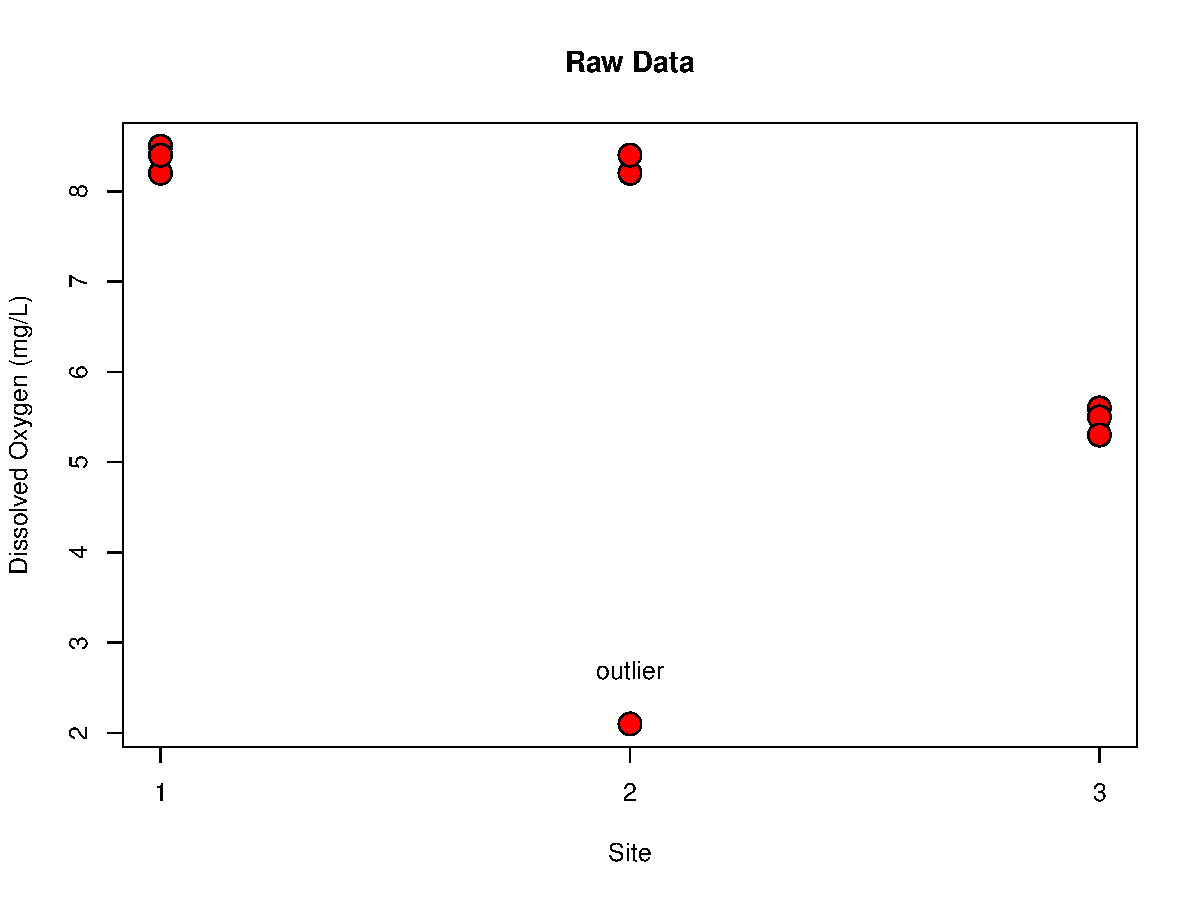
\includegraphics{./figures/badplots1.pdf}}
\end{center}

\vspace{-2ex}
{\scriptsize Here is an example where three measurements of dissolved
  oxygen were collected at three different sites.  This figure shows the
  actual measurements.  Can you describe the pattern?\\}
\end{frame}



\begin{frame}
\begin{center}
\resizebox{3.5in}{!}{
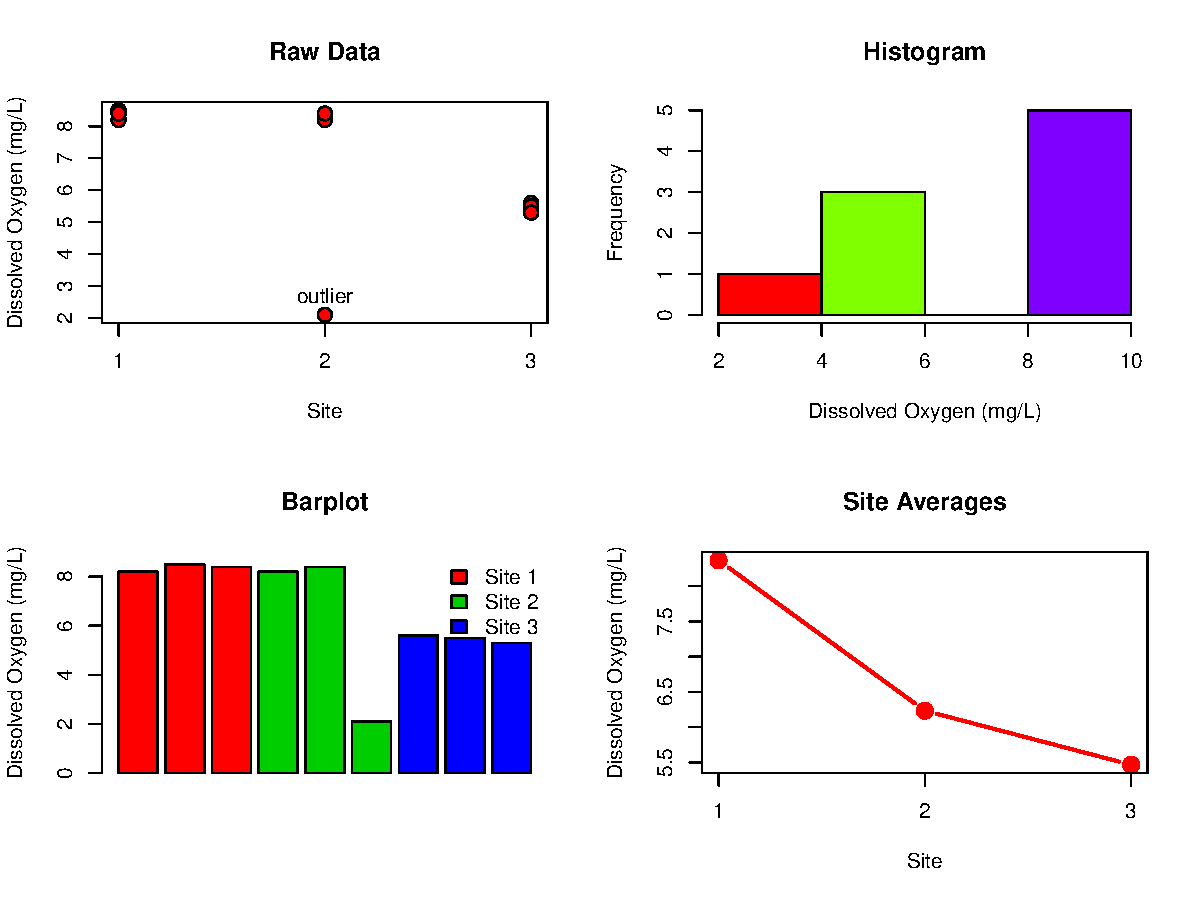
\includegraphics{./figures/badplots2.pdf}}
\end{center}

\vspace{-2ex}
{\scriptsize Here are the original data with three {\color{magenta}
 summary} plots, all of which are poor illustrations of how dissolved oxygen
 changes at the three sites\\}  
\end{frame}

\begin{frame}
\begin{center}
\resizebox{3.5in}{!}{
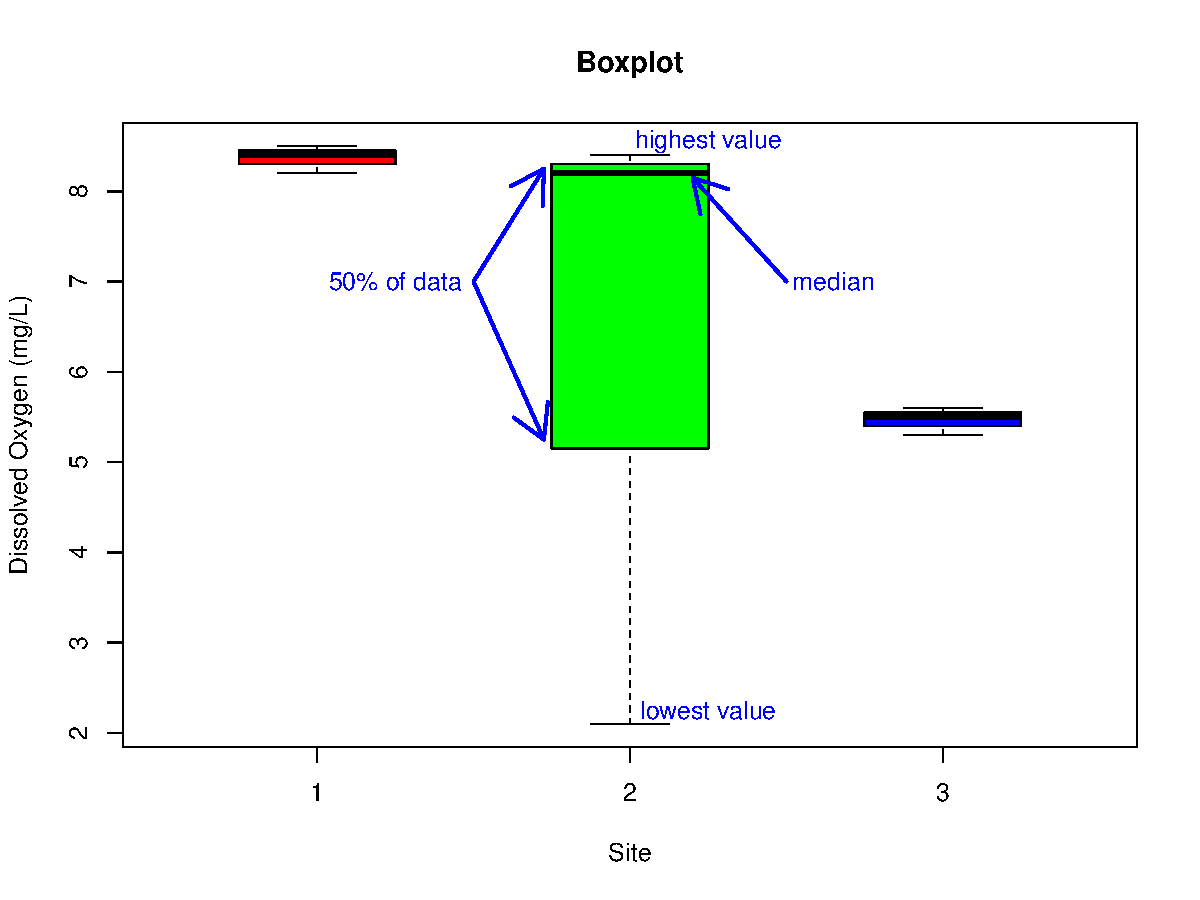
\includegraphics{./figures/goodplot.pdf}}
\end{center}

\vspace{-2ex}
{\scriptsize This {\color{magenta} \em boxplot} is a good scientific summary
 figure because it shows the influence of the outlier at Site 2 as well as the
 similarity between Site 1 and 2; however, it may not be the best way to
 summarize data to non-scientists\\}  
\end{frame}


\begin{frame}
\frametitle{Memory Used for Processing Visual Information}

{\small We use three basic types of memory to process
  scientific information:

      \bi
{\footnotesize
      \item {\color{blue} \em Iconic memory} for detecting visual information
            \bi
{\scriptsize
            \item {\em \color{magenta} Pre-attentive processing}\\
}
             \ei
 
     \item {\color{blue} \em Short-term memory} for temporary (limited)
        storage

            \bi
{\scriptsize
            \item {\color{magenta} \em Attentive or perceptual processing} 
            \item Limited to $\sim$ 3--9 items
}
            \ei

      \item {\color{blue} \em Long-term memory} for retaining information

            \bi
{\scriptsize
            \item Long-term memory can be created consciously or unconsciously
            
            \vspace{1ex}
            \item Information is stored more permanently, with cross-links
              that allow access back into short-term memory
            
            \vspace{1ex}
            \item Required for recognizing images, interpreting words and
              numbers, understanding context\\
}
            \ei
}
      \ei
}

\end{frame}



\begin{frame}
\frametitle{Pre-Attentive Processing of Visual Information}

\bi 
{\small
\item {\bf \color{blue} Pre-attentive processing} (iconic memory) provides
  quick, subconscious processing of graphical information and is influenced by variations in:
  \bi
  \item form
  \item color
  \item spatial position
  \item motion
  \ei

\vspace{2ex}
\item Graphics that make use of these features tend to make a strong
  impression on us, even when we don't know why\\

\vspace{2ex}
\item In creating visual displays of scientific information, the careful use
  of color, shape, position, and other design effects can {\bf \color{red}
  emphasize} or {\color{yellow} de-emphasize} information in the figure\\

}
\ei

\end{frame}




\begin{frame}
\frametitle{Pre-Attentive Processing}

{\footnotesize {\em \color{blue} Pre-attentive processing} involves high-speed,
subconscious processing of variations in form, color, spatial position, and
motion\\}

\begin{center}
\resizebox{3.25in}{!}{
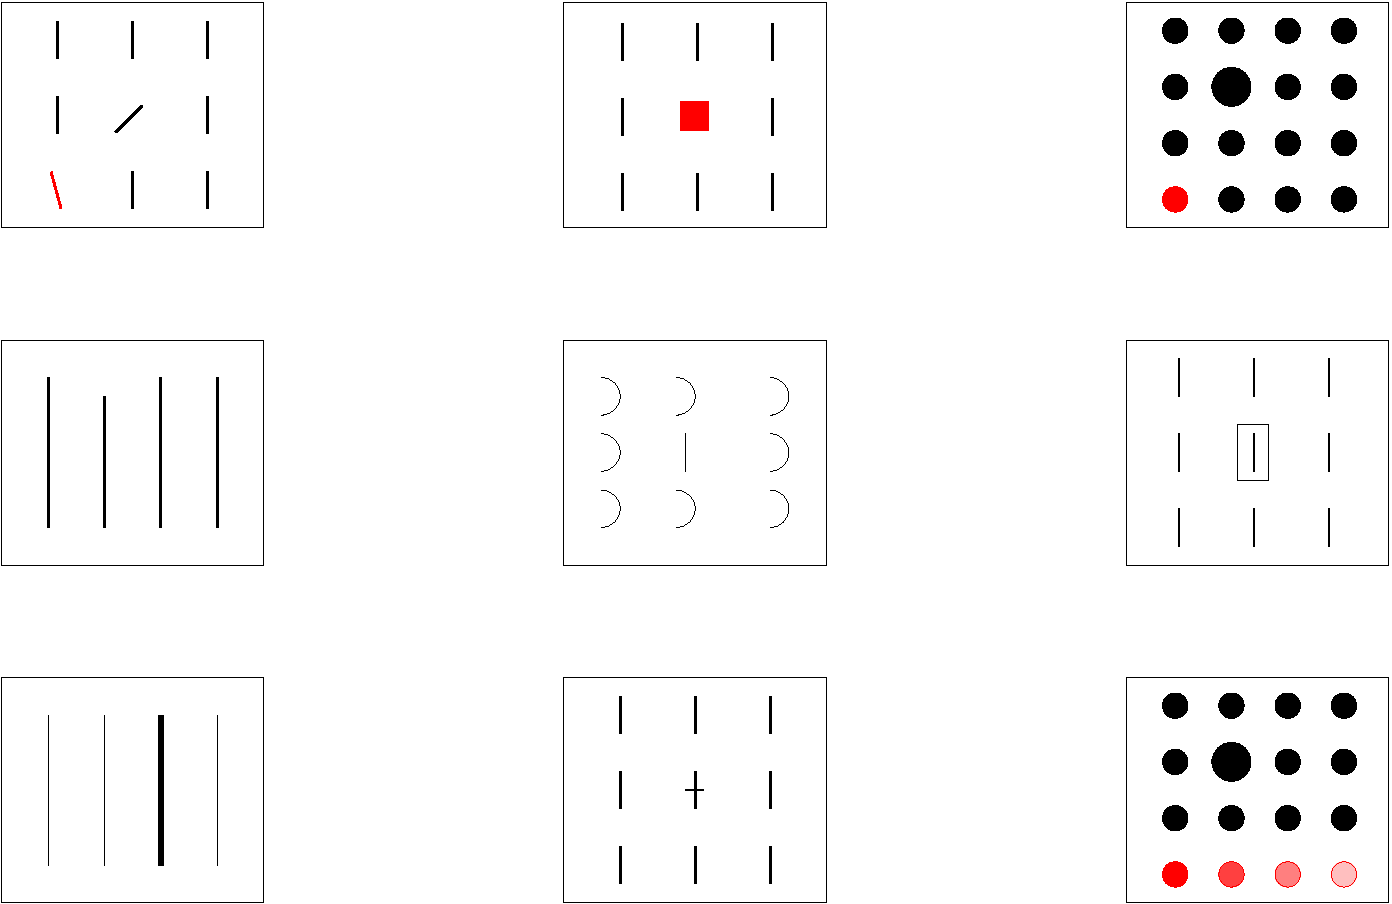
\includegraphics{./figures/form.pdf}}
\end{center}
{\scriptsize Figures modified from {\color{blue} Show Me The Numbers} by Stephen Few, Analytics Press, 2004\\ }
\end{frame}


\begin{frame}
\frametitle{Example using Color and Form}
{\scriptsize
\begin{center}
\begin{tabular}{cccccccccccc}
\multicolumn{12}{c}{How many zeros are there?}\\
6     & 4    & 4    & 2    & 1    & 5    & 7    & 2    & 2    & 2    & 2    & 8    \\
9     & 8    & 9    & 3    & 6    & 5    & 5    & 5    & 7    & 8    & 7    & 6    \\
1     & 3    & 5    & 9    & 5    & 6    & 0    & 6    & 7    & 6    & 6    & 6    \\
7     & 4    & 2    & 5    & 7    & 7    & 1    & 5    & 5    & 5    & 4    & 2   \\
5     & 2    & 1    & 1    & 4    & 2    & 6    & 6    & 4    & 9    & 6    & 3    \\
5     & 7    & 2    & 0    & 6    & 1    & 6    & 8    & 0    & 6    & 0    & 2    \\
9     & 8    & 7    & 4    & 4    & 5    & 4    & 4    & 9    & 1    & 5    & 1    \\
2     & 1    & 3    & 7    & 8    & 6    & 2    & 0    & 2    & 9    & 4    & 9    \\
3     & 4    & 9    & 6    & 2    & 1    & 7    & 9    & 4    & 8    & 2    & 8    \\
2     & 5    & 5    & 2    & 2    & 4    & 5    & 5    & 8    & 7    & 1    & 5    \\
\end{tabular}
\end{center}
}

{\scriptsize
\begin{center}
\begin{tabular}{cccccccccccc}
\multicolumn{12}{c}{How many zeros are there?}\\
6     & 4    & 4    & 2    & 1    & 5    & 7    & 2    & 2    & 2    & 2    & 8    \\
9     & 8    & 9    & 3    & 6    & 5    & 5    & 5    & 7    & 8    & 7    & 6    \\
1     & 3    & 5    & 9    & 5    & 6    & {\large \bf \color{red}0}    & 6    & 7    & 6    & 6    & 6    \\
7     & 4    & 2    & 5    & 7    & 7    & 1    & 5    & 5    & 5    & 4    & 2   \\
5     & 2    & 1    & 1    & 4    & 2    & 6    & 6    & 4    & 9    & 6    & 3    \\
5     & 7    & 2    & {\large \bf \color{red}0}    & 6    & 1    & 6    & 8    & {\large \bf \color{red}0}    & 6    & {\large \bf \color{red}0}    & 2    \\
9     & 8    & 7    & 4    & 4    & 5    & 4    & 4    & 9    & 1    & 5    & 1    \\
2     & 1    & 3    & 7    & 8    & 6    & 2    & {\large \bf \color{red}0}    & 2    & 9    & 4    & 9    \\
3     & 4    & 9    & 6    & 2    & 1    & 7    & 9    & 4    & 8    & 2    & 8    \\
2     & 5    & 5    & 2    & 2    & 4    & 5    & 5    & 8    & 7    & 1    & 5    \\
\end{tabular}
\end{center}
}

{\scriptsize Here is an example of how pre-attentive color processing helps clarify tabular information\\}

\end{frame}


\begin{frame}

\frametitle{Perceptual Processing of Visual Information}

\bi 
{\footnotesize
\item {\bf \color{red} Perceptual processing} (conscious interpretation of
  visual information) is based on perceptions of difference rather than the
  ability to recognize absolute values
  
\vspace{1ex}
\item As a result, it is quite easy to fool our visual perception of data
using simple optical tricks and illusions

\vspace{1ex}
\item Some of the best examples of this are found in advertising

   \bi
{\scriptsize
   \item One trick for {\color{blue} staging} houses for sale involves
   tricking our perception of room size by adding mirrors, light colored
   paint, and removing most of the furniture to make rooms look larger

\vspace{1ex}
   \item Another advertising trick is to place warnings or qualifying
   information at the bottom of the screen in small, light colored lettering,
   against a backdrop of screen motion.  (Just {\em try} to stay focused on
   the text at the bottom of your TV screen!)\\
}
\ei

\vspace{1ex}
\item Perceptual processing in essential for understanding data in tables and written discussion,
  but remember that it can slow down our ability to interpret information\\
}
\ei

\end{frame}


\begin{frame}
\frametitle{Designing Effective Figures}
\framesubtitle{Example \#1 - Drayton Harbor Coliforms}

\begin{center}
\resizebox{3.5in}{!}{
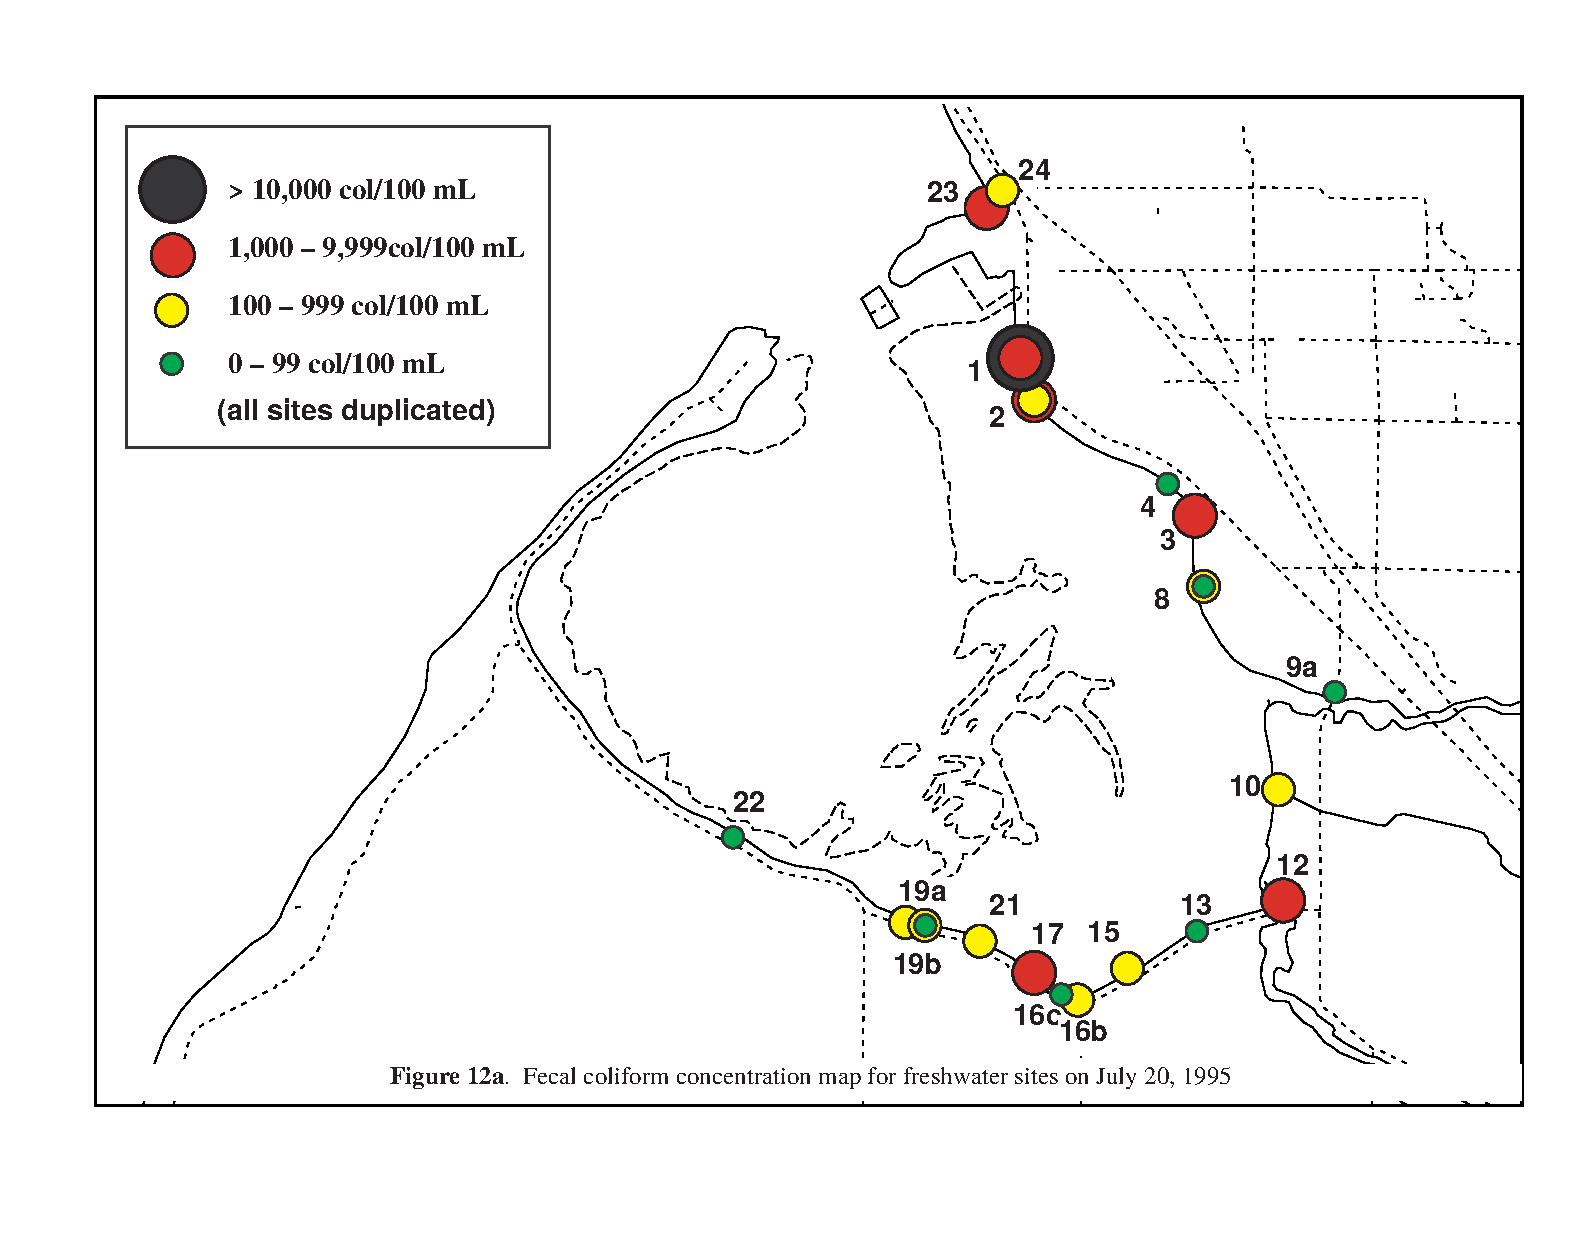
\includegraphics{./figures/harbor_7_20.pdf}}
\end{center}

\vspace*{-5ex}
        {\scriptsize This figure has a few bad features (e.g., key is distracting),
  but uses pre-attentive processing techniques effectively\\}
\end{frame}


\begin{frame}
\frametitle{Designing Effective Figures}
\framesubtitle{Example \#1, continued}

\begin{center}
\resizebox{3.5in}{!}{
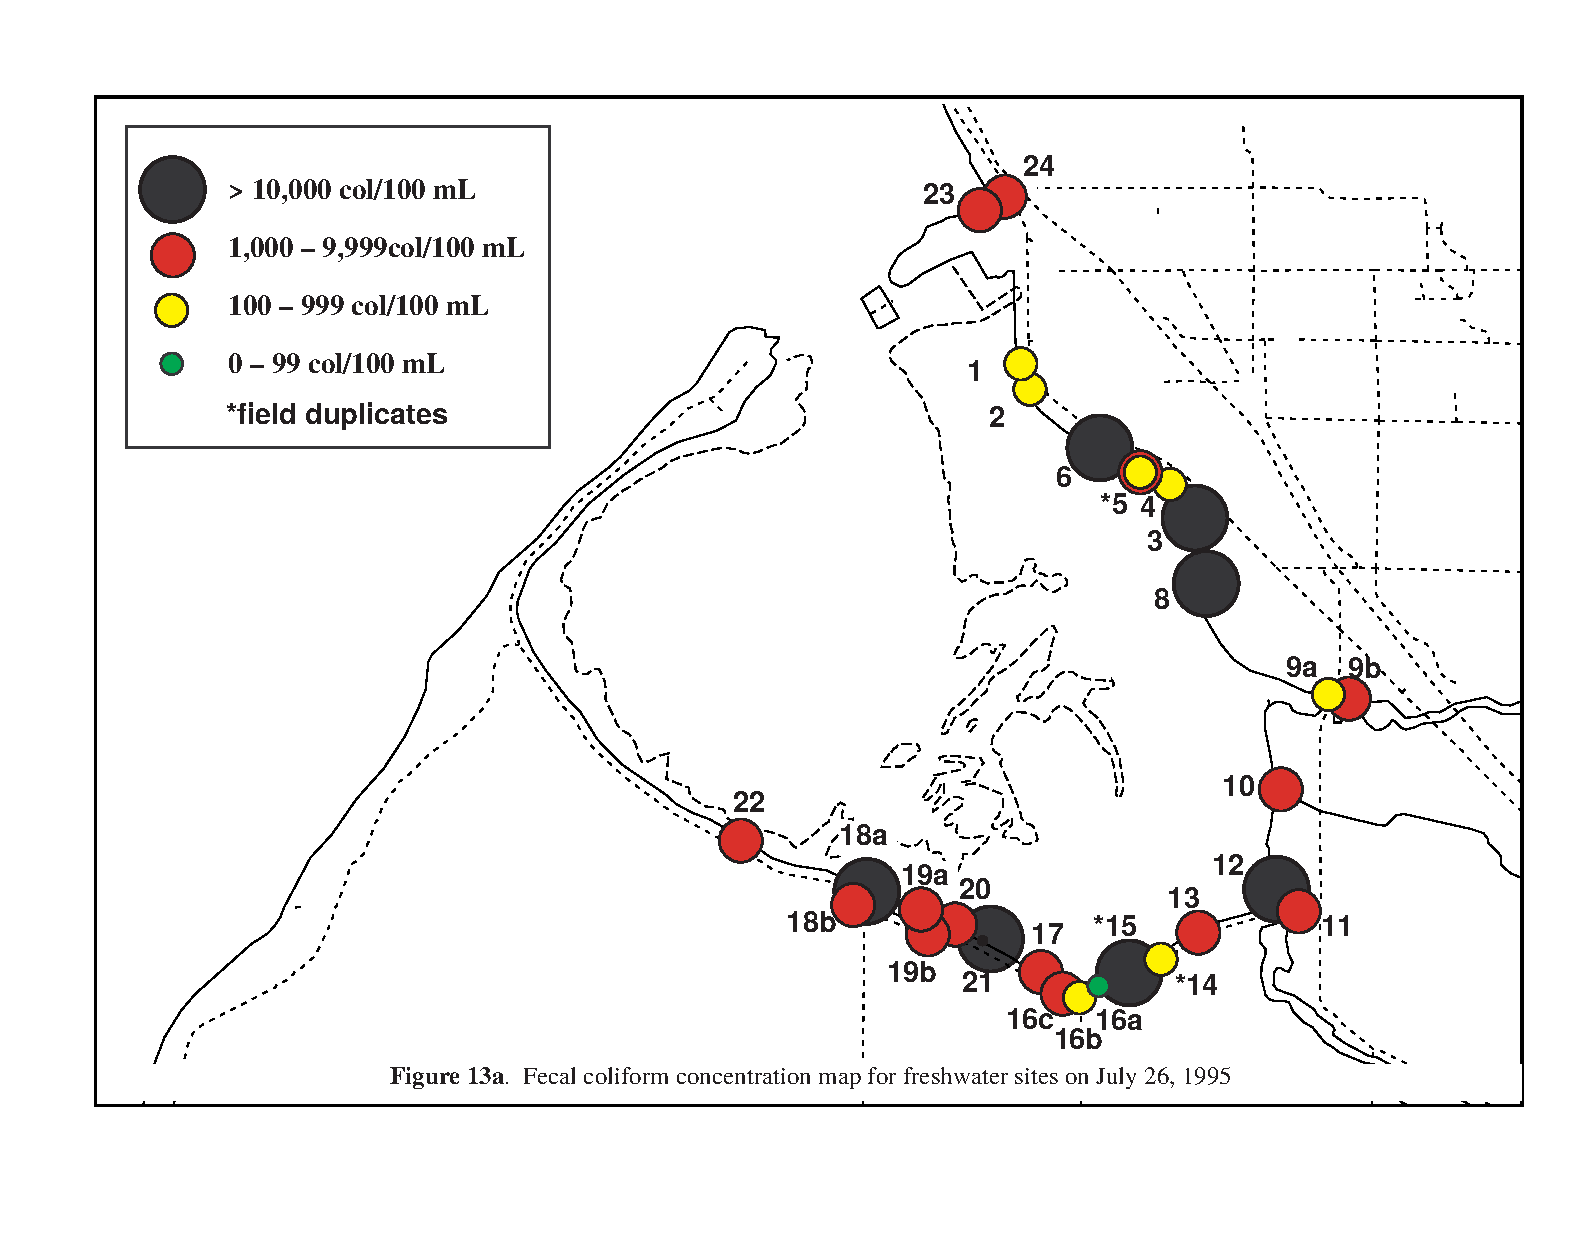
\includegraphics{./figures/harbor_7_26.pdf}}
\end{center}

\vspace*{-5ex}
{\scriptsize Note how the large red and black circles emphasize the much higher coliform
  counts on July 26 compared to July 20\\}
\end{frame}


\begin{frame}
\frametitle{Designing Effective Figures}
\framesubtitle{Example \#2, Padden Creek Sediments}

\begin{center}
\resizebox{3in}{!}{
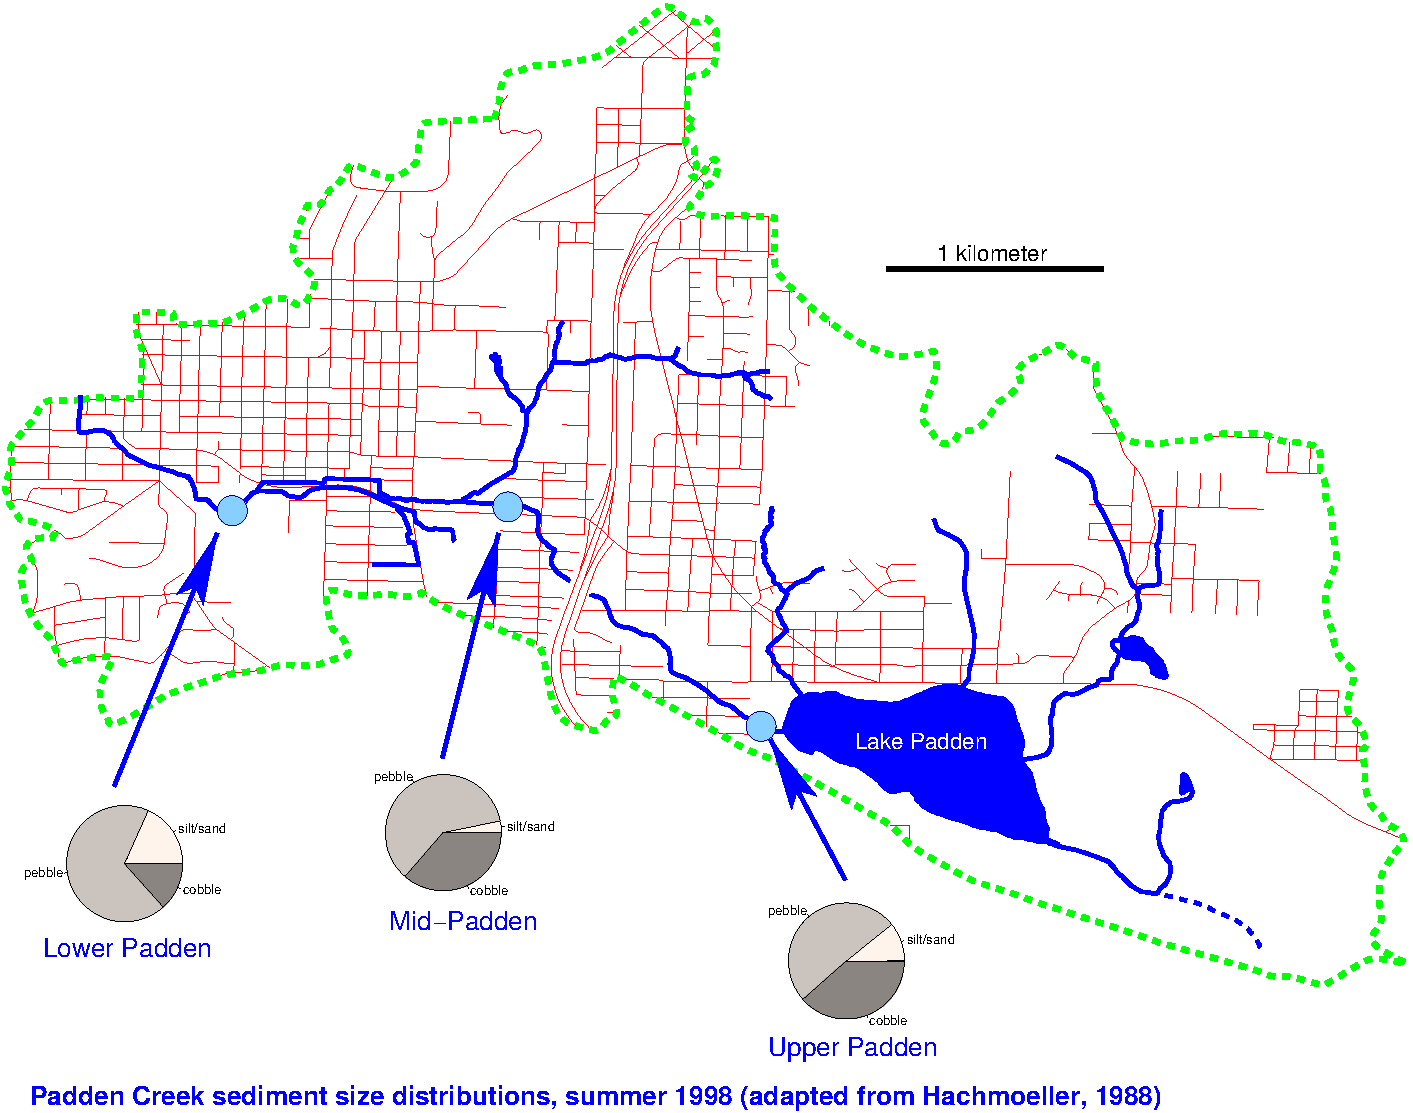
\includegraphics{./figures/padden.pdf}}
\end{center}

\vspace*{-2ex}
{\scriptsize Here is example that uses boxplots to display data.  What are other options for presenting the information?\\}
\end{frame}


\begin{frame}
\frametitle{Designing Effective Figures}
\framesubtitle{Example \#3, Nitrate Levels in Abbotsford/Sumas Wells}

\vspace*{-2ex}
\begin{center}
\resizebox{3in}{!}{
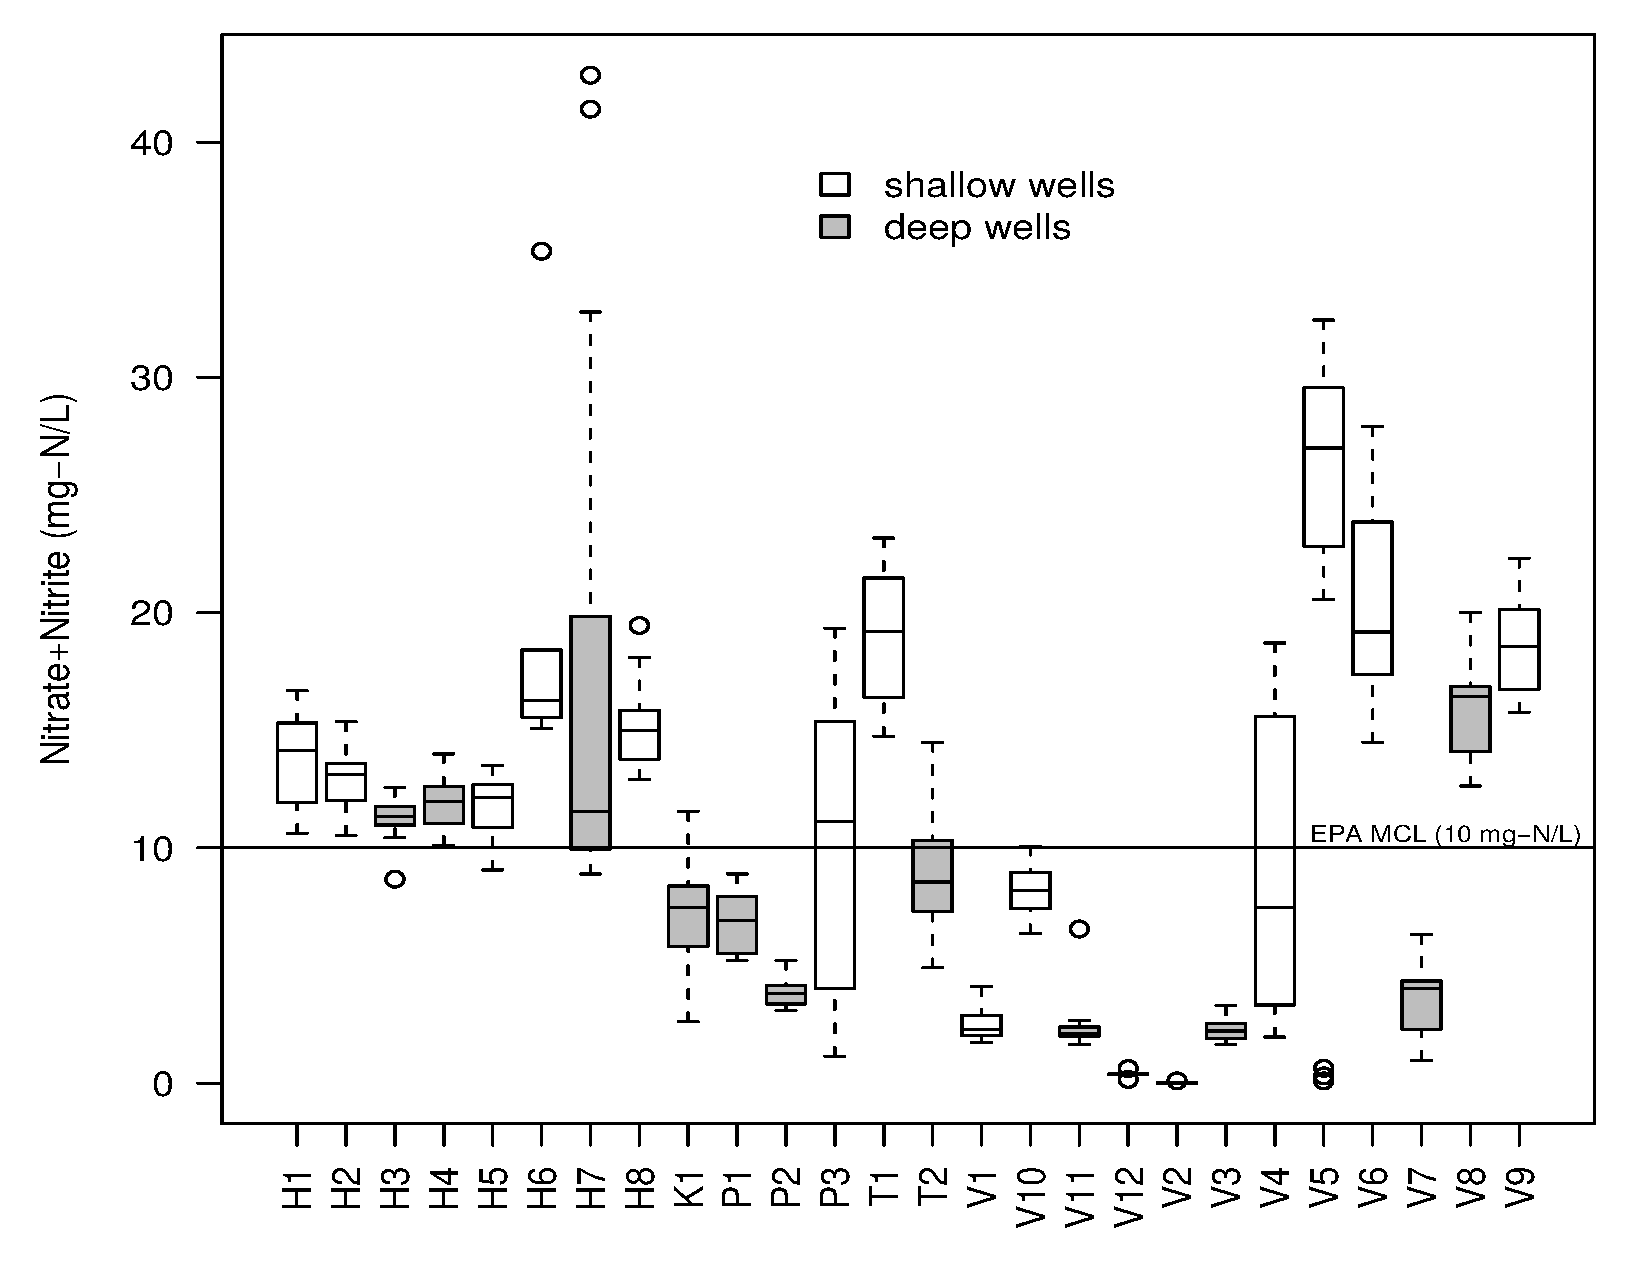
\includegraphics{./figures/AS_nitrate.pdf}}
\end{center}

\vspace*{-2ex}
{\scriptsize This figure contains a large amount of summary information.  What can
  you determine from the graphics?\\}

\end{frame}


\begin{frame}
\frametitle{Designing Effective Figures}
\framesubtitle{Example \#4 - Are Cyanobacteria Increasing in Lake Whatcom?}

\vspace*{-0.15in}
\begin{center}
\resizebox{2.5in}{!}{
	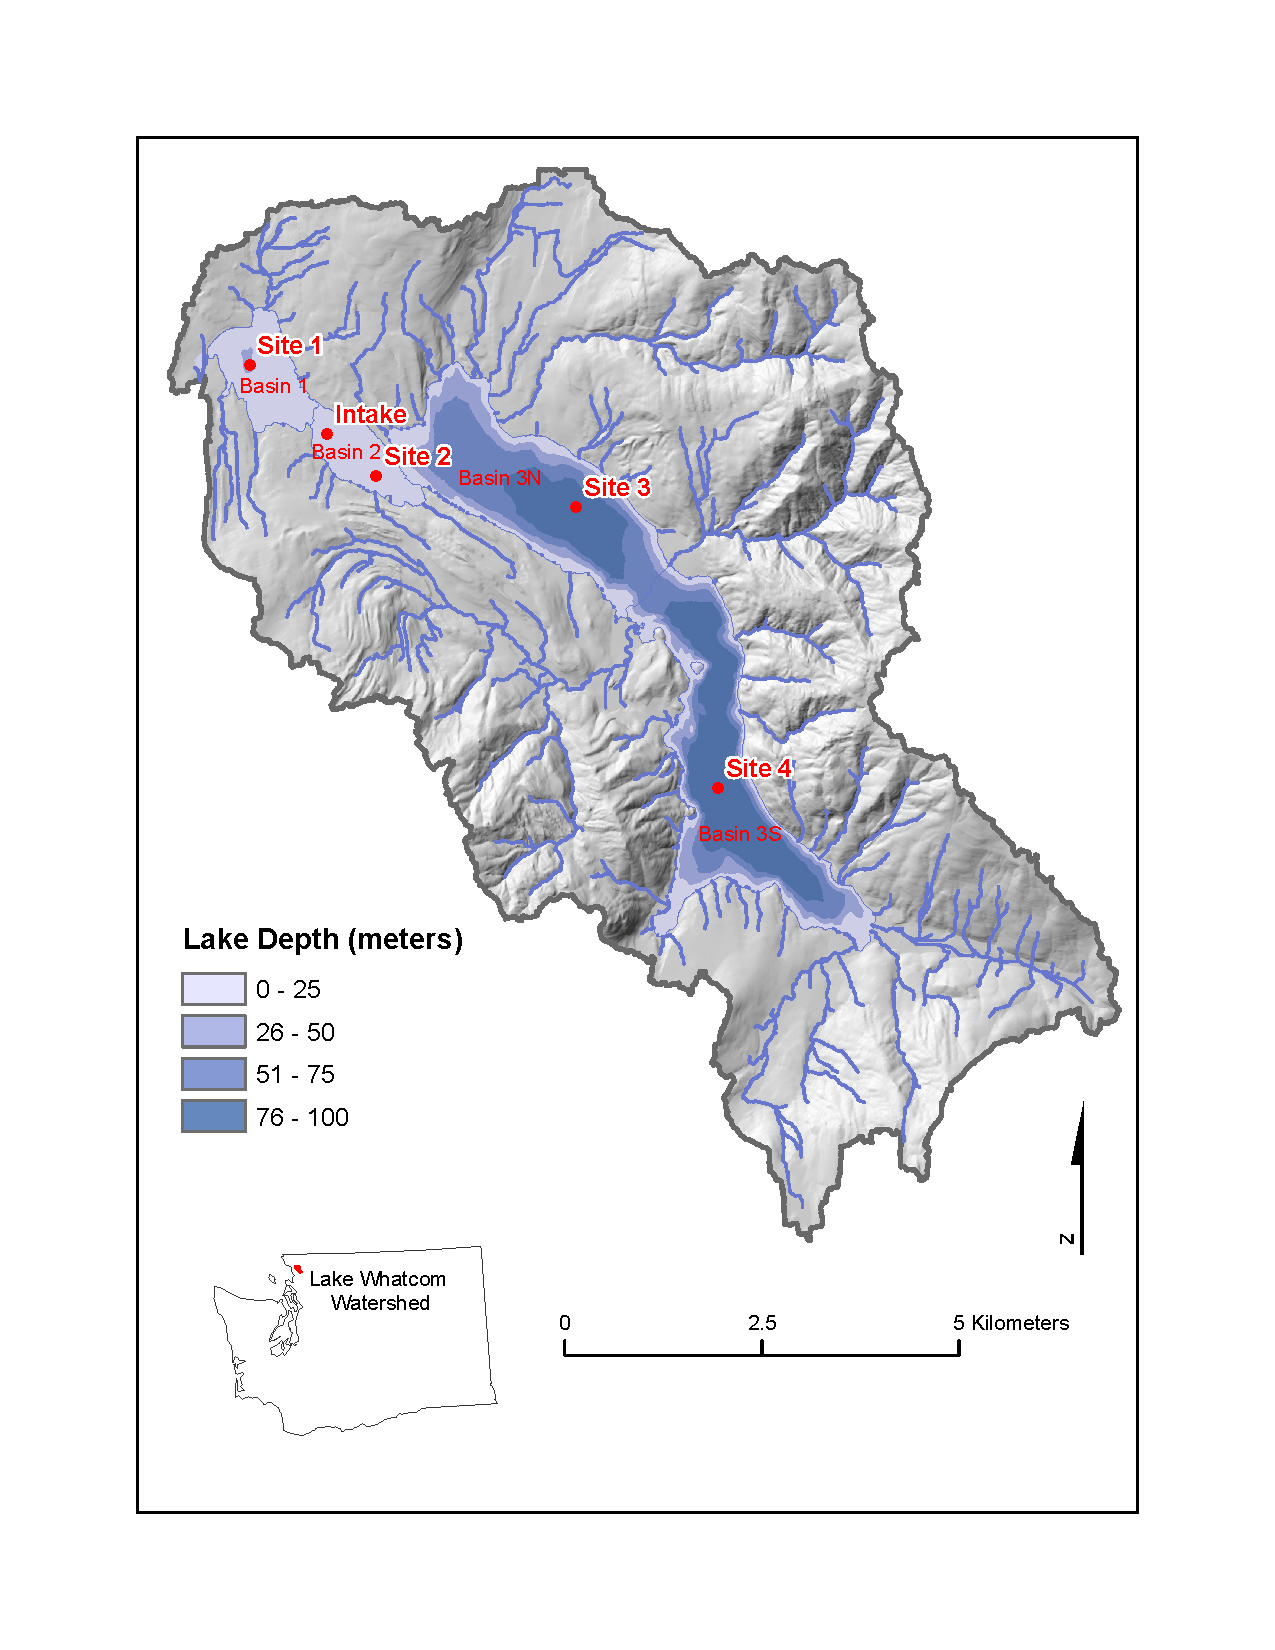
\includegraphics{./figures/Fig1a.pdf}}
\end{center} 
\end{frame}


\begin{frame}
\frametitle{Designing Effective Figures}
\framesubtitle{Example \#4, Scientific background:}

  \bi
\item Cyanobacteria (aka bluegreen algae) are water quality indicators
  that often increase in abundance in polluted lakes

\vspace{1ex}
\item Researchers associated with Western Washington University have
been counting algae in Lake Whatcom for more than 20 years

\vspace{1ex}
\item Algae samples were collected monthly (except Jan and Mar) at 5 meters
  below the surface at four sites in the lake as part of a long-term
  monitoring project

\bi
{\scriptsize
\item Prior to 1994, most of the counts were collected by graduate students,
  with minimal coordination between different individuals.  After 1994, the
  counts followed a more consistent procedure\\}
\ei

\vspace{1ex}
\item Intensive sampling (more depths, more sites, more frequent sampling) has
  been done by various researchers, but the data are sporadic and there is
  little, if any, similarity between methods
\ei

\end{frame}


\begin{frame}
\frametitle{Designing Effective Figures}
\framesubtitle{Example \#4 - Preliminary Data Analysis Decisions}

Assessing long term trends requires that we isolate ``time'' as the
factor influencing algae counts, and reduce or eliminate other factors
that might cause changes in the counts

\bi
\item {\color{red} Decision \#1:}  Use data beginning in 1994 to minimize
  influence of different counting techniques

\vspace{1ex}
\item {\color{red} Decision \#2:}  Use data from monthly sampling
  to minimize influence of different sampling intensities

\vspace{1ex}
\item {\color{red} Decision \#3:} Use data from Sites 1--4 collected 5 meters
  below the surface to minimize differences due to depth and location in the lake
\ei

\end{frame}


\begin{frame}
\begin{center}
\resizebox{3.5in}{!}{
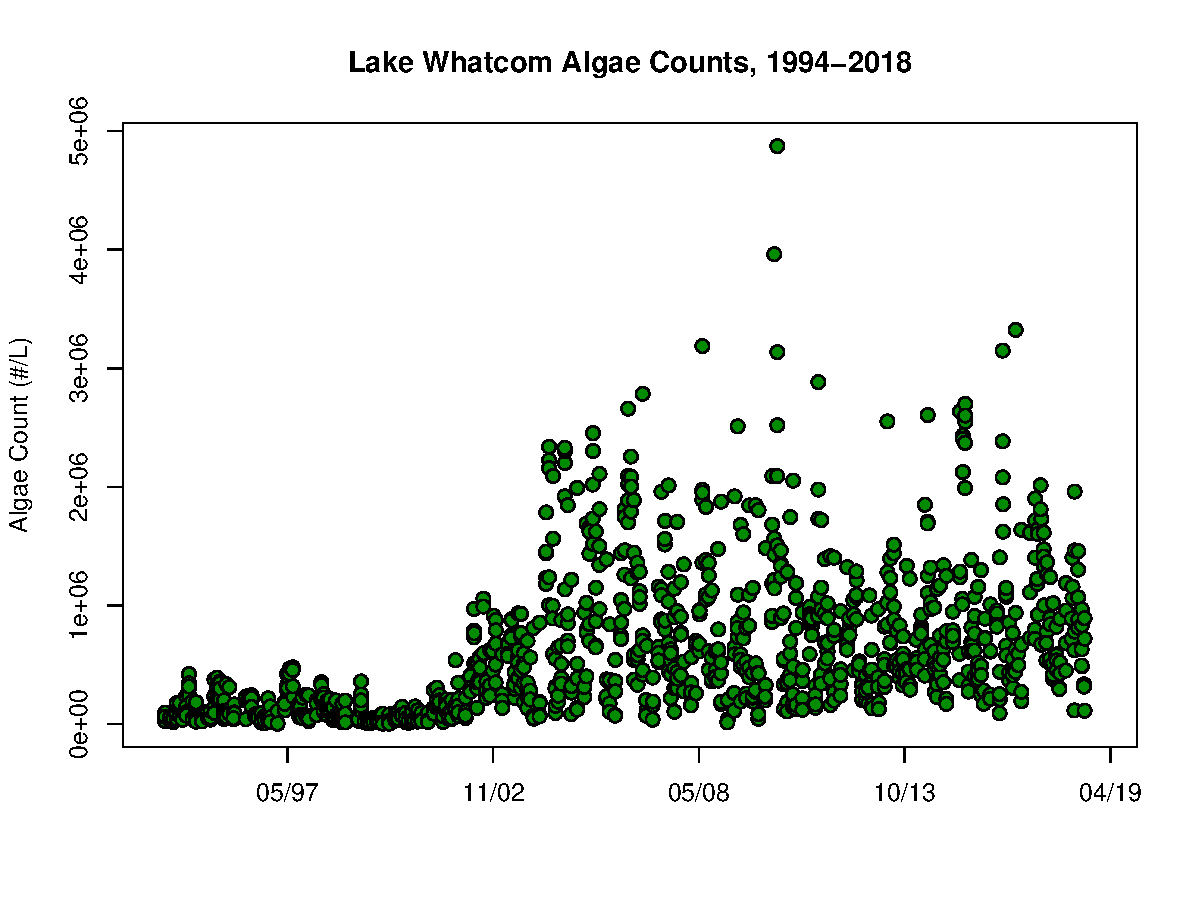
\includegraphics{./figures/algae1.pdf}}
\end{center}

\vspace{-2ex}
{\scriptsize Here is a plot of the raw algae counts from 1994--2018,
  without distinguishing site or type of algae.  (Remember, our goal is to say
  whether the bluegreen algae are increasing, not whether all algae are increasing)\\}
\end{frame}


\begin{frame}
\begin{center}
\resizebox{3.5in}{!}{
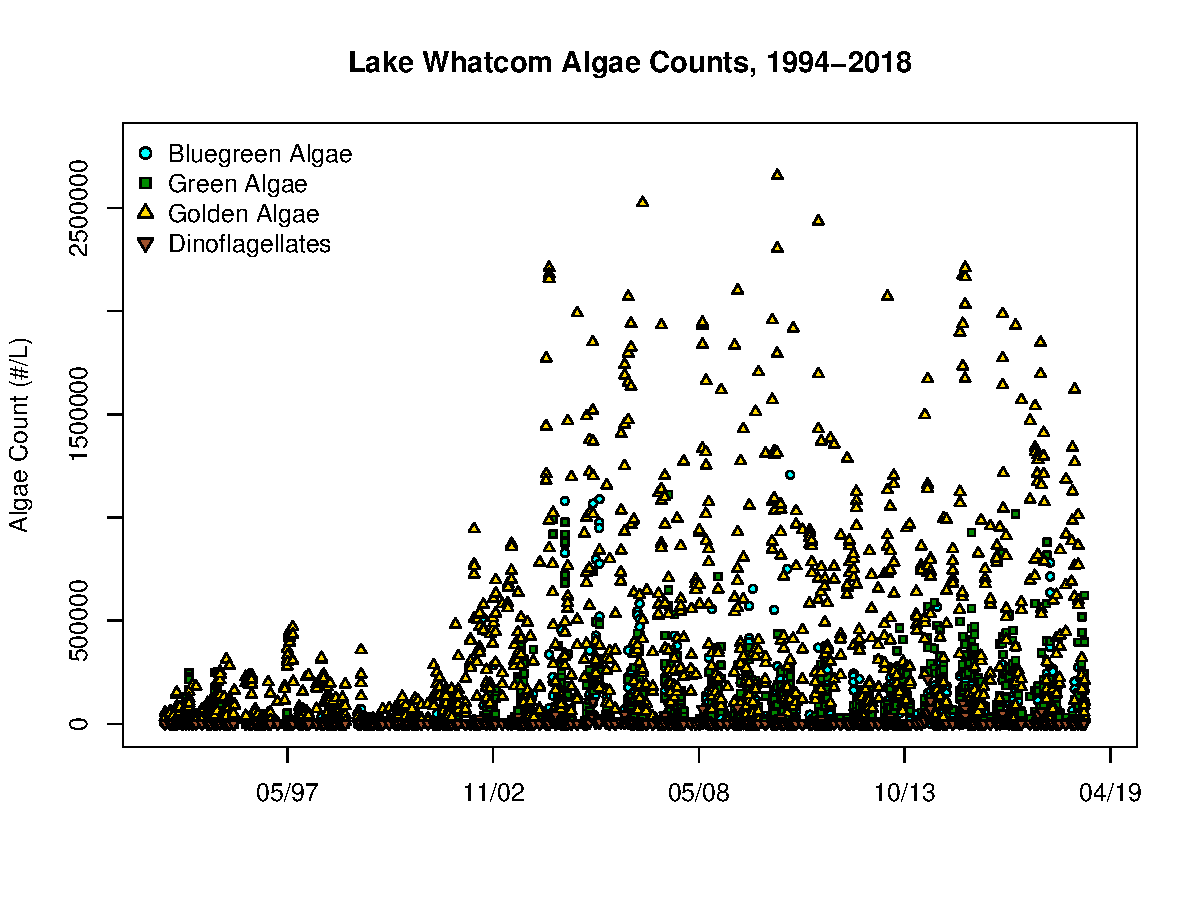
\includegraphics{./figures/algae2.pdf}}
\end{center}

\vspace{-2ex}
{\scriptsize If we assign plotting codes to separate the bluegreen
  algae from the other major algal types, we begin to see a potential
  problem.  Bluegreens are not the dominant type of algae in the lake $\ldots$
  golden algae (diatoms) are much more abundant.  Also, algal counts are very
  ``noisy'' (the counts have a large range)\\}
\end{frame}

\begin{frame}
\begin{center}
\resizebox{3.5in}{!}{
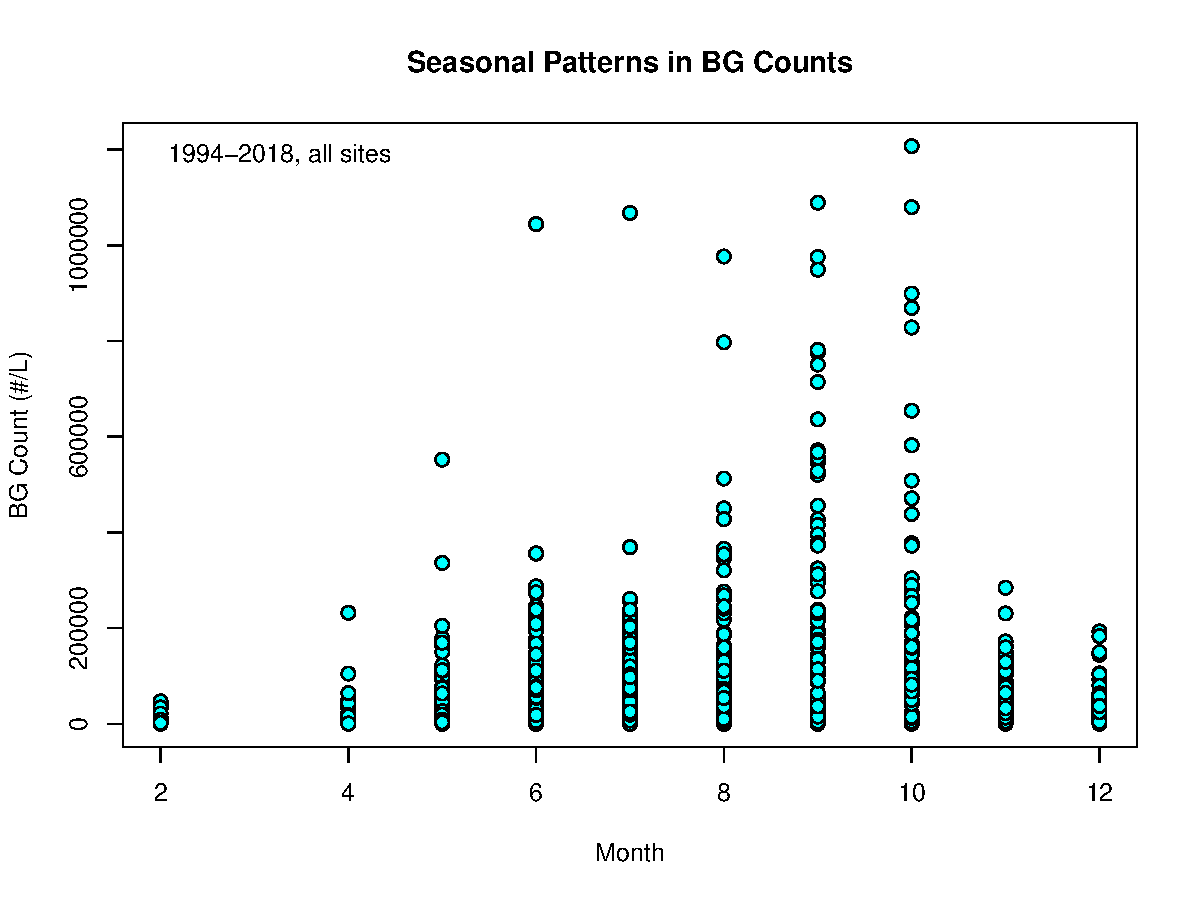
\includegraphics{./figures/algae6.pdf}}
\end{center}

\vspace{-2ex}
{\scriptsize Here is another problem: the previous figures
  included counts from all months and depths.  Bluegreen algae
  are only abundant in near the lake surface during summer and early fall\\}

\vspace{0.5ex}
{\scriptsize \color{red} One
  of the easiest ways to eliminate a trend is to average in data that you know
  won't show any patterns\\}
\end{frame}

\begin{frame}
\begin{center}
\resizebox{3.5in}{!}{
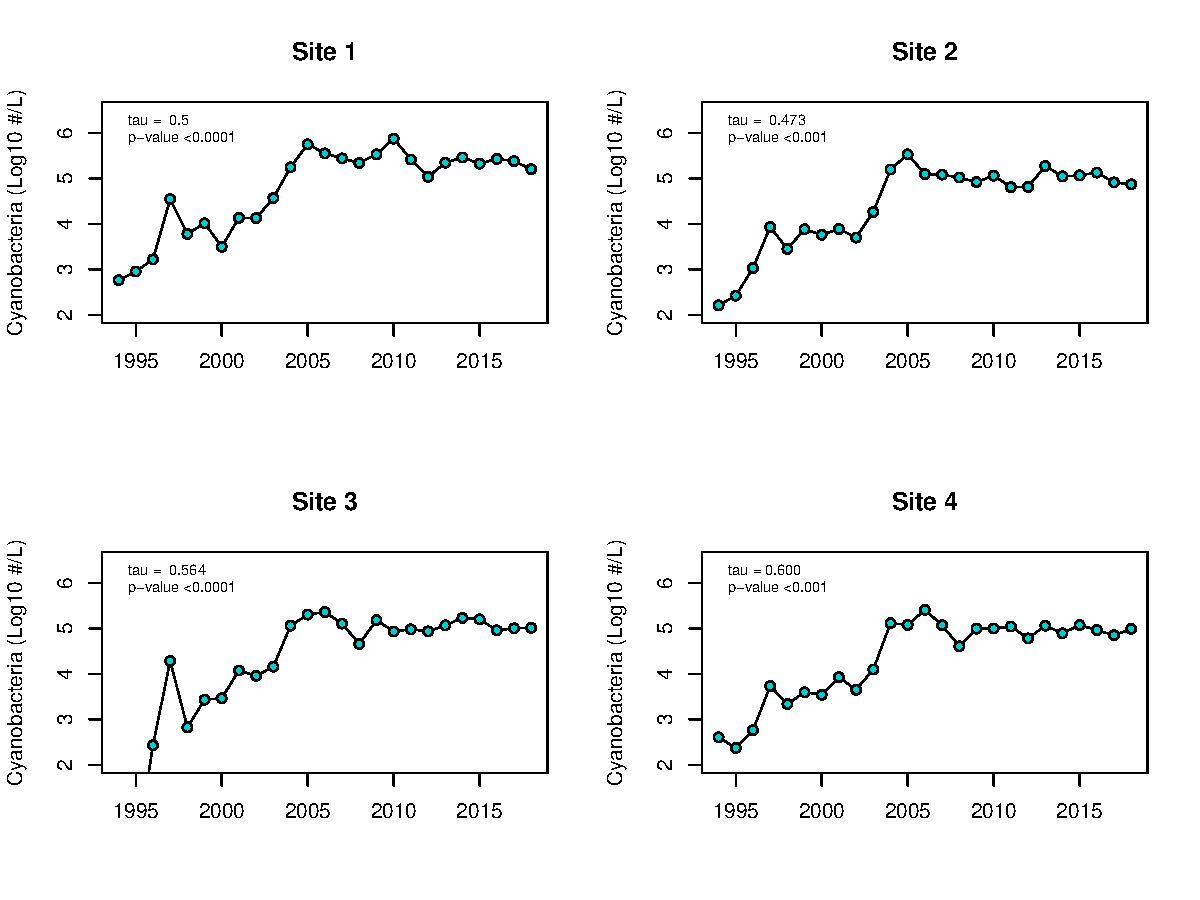
\includegraphics{./figures/algae9.pdf}}
\end{center}

\vspace{-2ex} {\scriptsize Here are the figures used for the annual
  reports, showing near-surface medians (June-October, $\le$5 meters),
  with correlation results confirming that cyanobacteria are
  increasing significantly with time. Three items should be apparent:
  the cyanobacteria counts increased between 1994 and 2005; the
  correlation with year is strongest at Sites 3--4; the counts have
  been stable for about half the time period, so the statistical
  analysis {\em should} be divided into pre- and post-2005\\}
\end{frame}

\begin{frame}
\frametitle{Designing Effective Figures}
\framesubtitle{Example \#5 - Are Temperature and Oxygen Levels Changing in Lake Whatcom?}

\bi
\item Preliminary data from the early 1990s suggested that oxygen
  concentrations were declining near the bottom of Lake Whatcom

\vspace{0.5ex}
\item Researchers associated with Western Washington University have
been collecting temperature and oxygen data in Lake Whatcom since the 1960s

\vspace{0.5ex}
\item  Beginning in late 1989, the sampling and analysis methods were standardized
  \bi
  \item {\color{red} Decision \#1:} Use data collected from 1990 to ensure similar sample sizes for all years
  \ei
\ei

\end{frame}


\begin{frame}
\frametitle{Lake Whatcom Temperature and Oxygen Data}

\begin{center}
\resizebox{2.5in}{!}{
	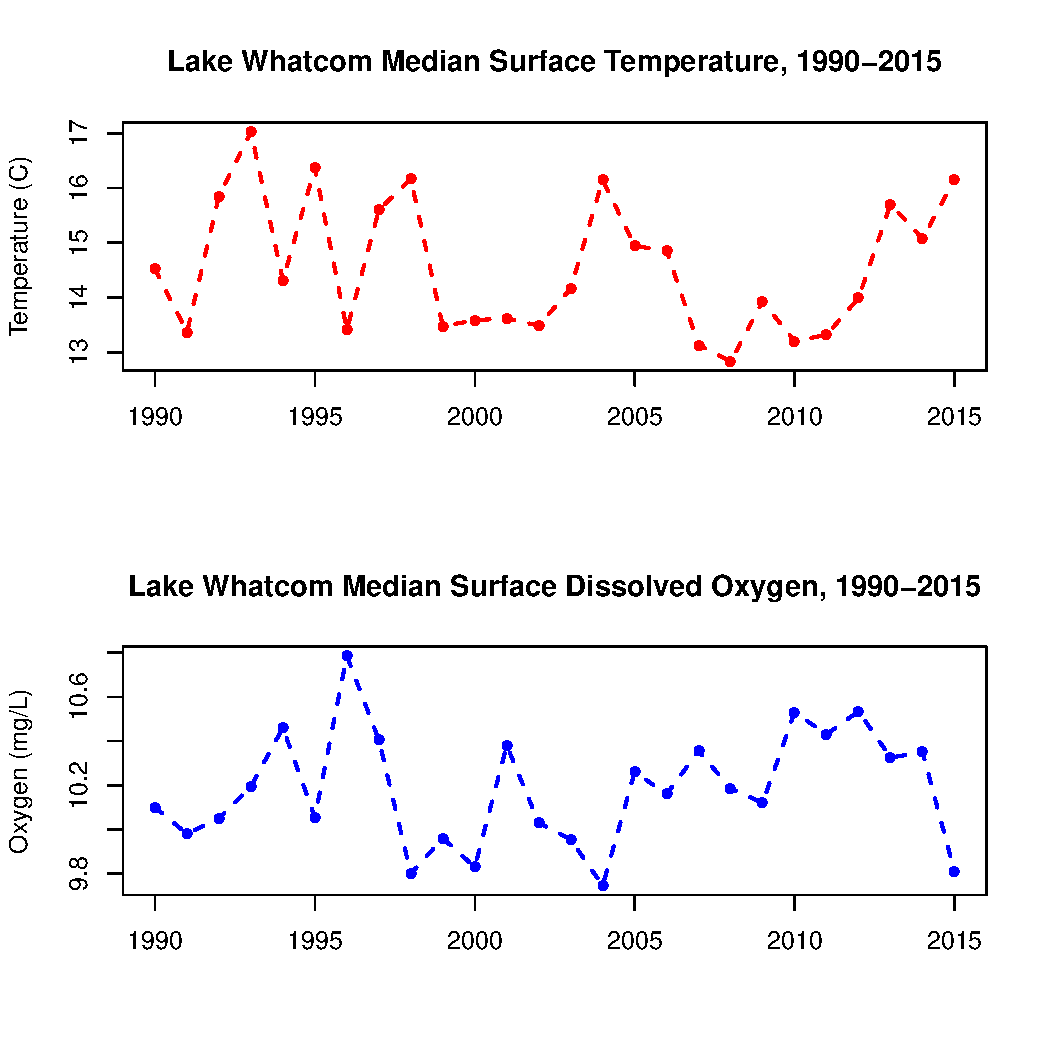
\includegraphics{./figures/simple.pdf}}
\end{center} 

\vspace*{-4ex}
{\scriptsize Here is an example using simple x-y scatterplots to look for
  patterns in Lake Whatcom surface temperature and
  dissolved oxygen levels.  This figure shows median surface
  temperature and oxygen levels for all sites and months ($\sim$40
  samples per year)\\}

\end{frame}

\begin{frame}
\frametitle{Lake Whatcom Temperature Data}
\framesubtitle{Influence of Spatial Location Revealed Using Trend Lines}
\begin{center}
\resizebox{3in}{!}{
	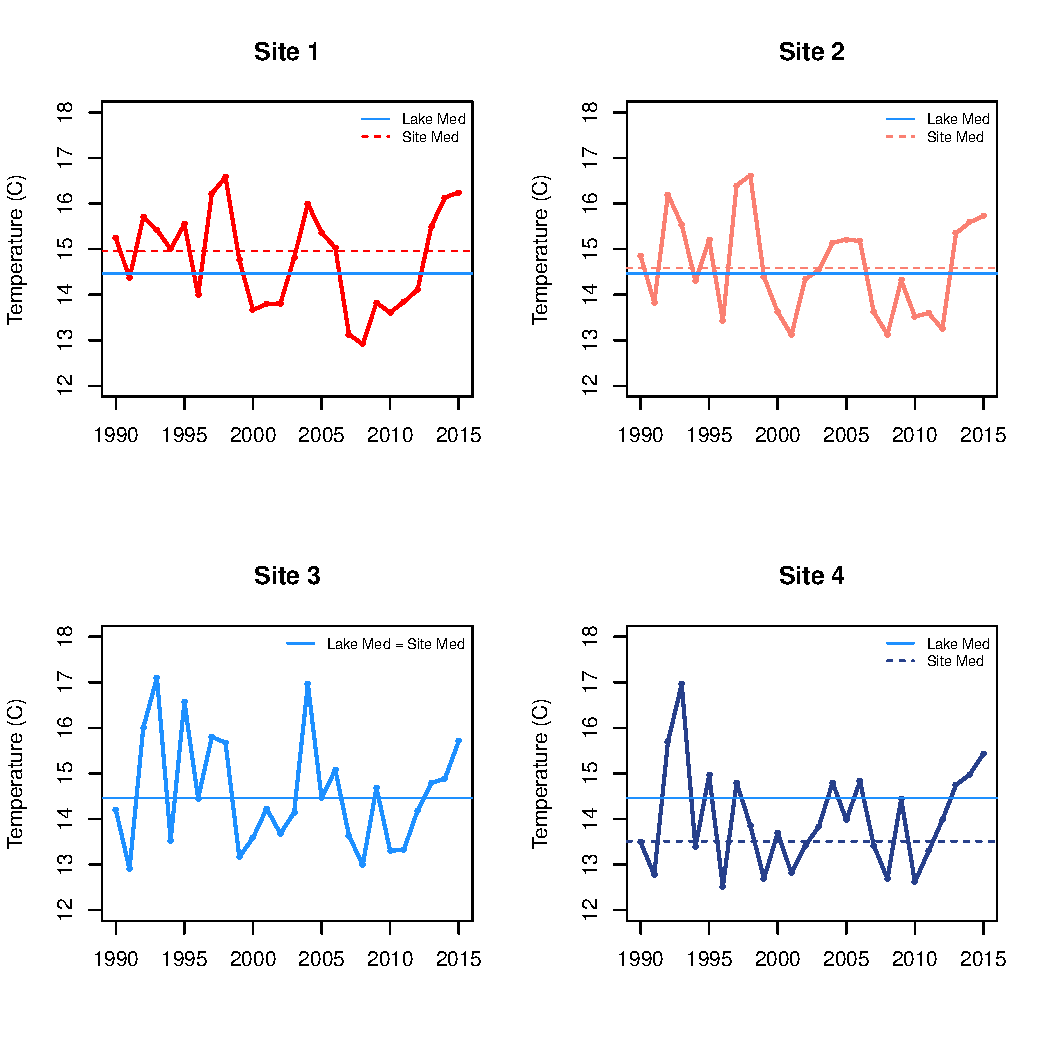
\includegraphics{./figures/simple3.pdf}}
\end{center}
\end{frame}


\begin{frame}
\frametitle{Lake Whatcom Oxygen Data}
\framesubtitle{Influence of Spatial Location Revealed Using Trend Lines}
\begin{center}
\resizebox{3in}{!}{
	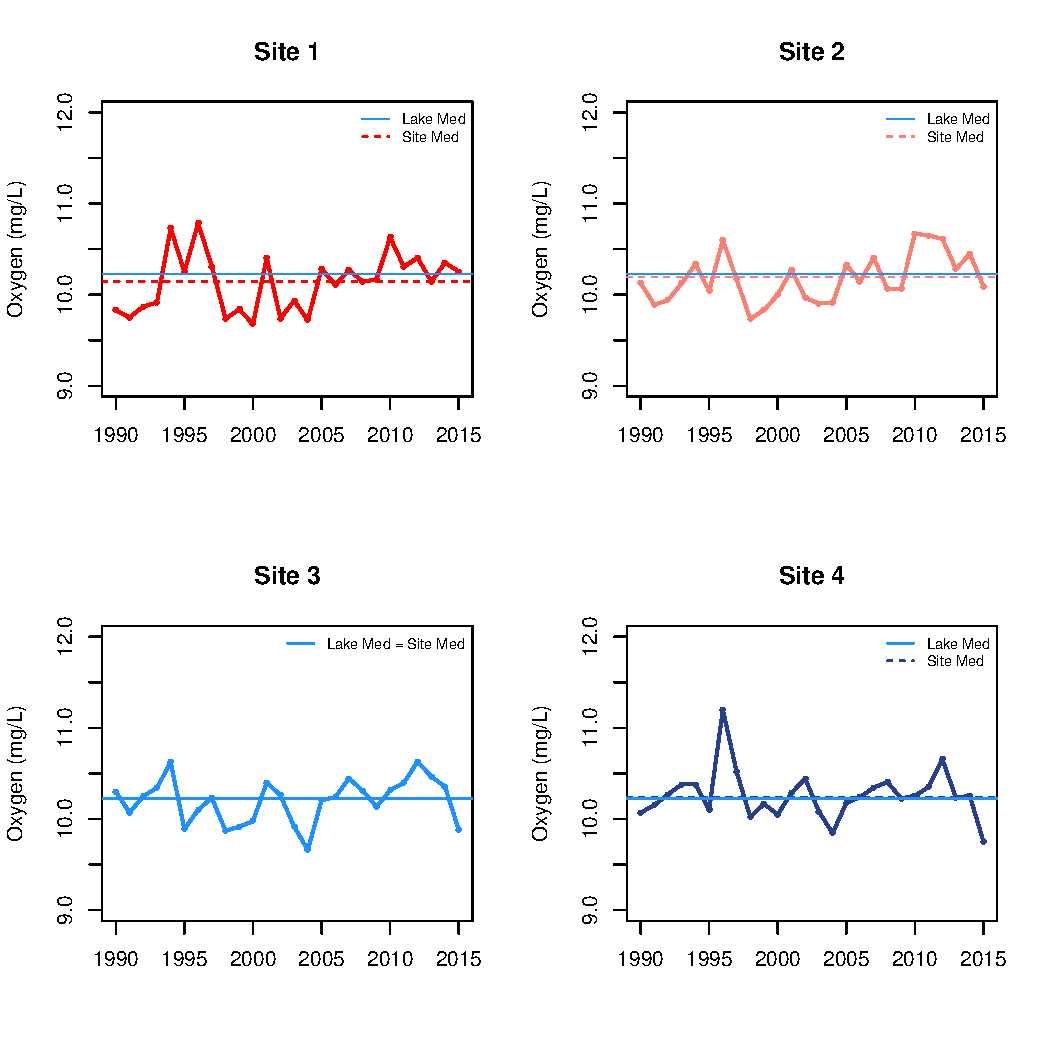
\includegraphics{./figures/simple4.pdf}}
\end{center}
\end{frame}


\begin{frame}
\frametitle{Lake Whatcom Temperature and Oxygen Data}
\framesubtitle{Example \#5, continued}

{\footnotesize
  \bi
\item The lake is very large and deep ($>$100 meters).  The majority
  of the lake (96\%) maintains consistently high oxygen concentrations

\vspace{1ex}
\item The temperature data, dating back to the 1960s, do not show a
  clear trend
  
\vspace{1ex}
\item The shallow sites (Sites 1--2), which are from basins that collectively represent
  only 4\% of the lake volume, both experience severe oxygen depletion during the summer
  
\vspace{1ex}
\item Only Site 1 appears to have decreasing oxygen concentrations,
  and this was only present in summer and late fall in samples from $>$10 meters deep
  
\vspace{1ex}
\item {\color{red} Decision \#2:} Use oxygen data collected at Site 1
  during the period of lake stratification. Oxygen data from 1988-1989
  can be included with these selection criteria
  \ei
}
\end{frame}


%%% created with xfig
\iwsframe{Lake Whatcom Oxygen Data}{3D Plot of Oxygen, Depth, and Time (1987--1989)}
\begin{center}
\resizebox{3.5in}{!}{
	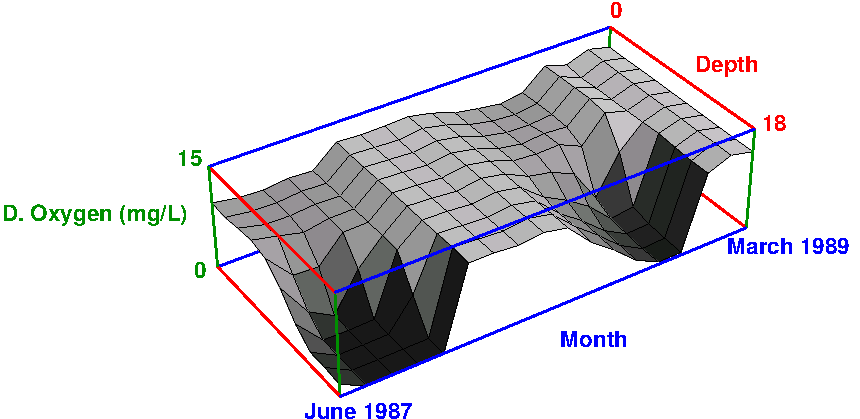
\includegraphics{./figures/ddo11.pdf}}
\end{center}

{\scriptsize This figure shows Lake Whatcom dissolved oxygen at Site 1 by
  time and depth for two sequential summers.  Although this figure
  reveals some seasonal and depth-related differences, the patterns are
  {\color{red} $\Rightarrow$}difficult to interpret\\}
\end{frame}


%% created with xfig
\iwsframe{Lake Whatcom Oxygen Data}{3D Plot of Oxygen, Depth, and Time (1988--2001)}
\begin{center}
\resizebox{3.25in}{!}{
	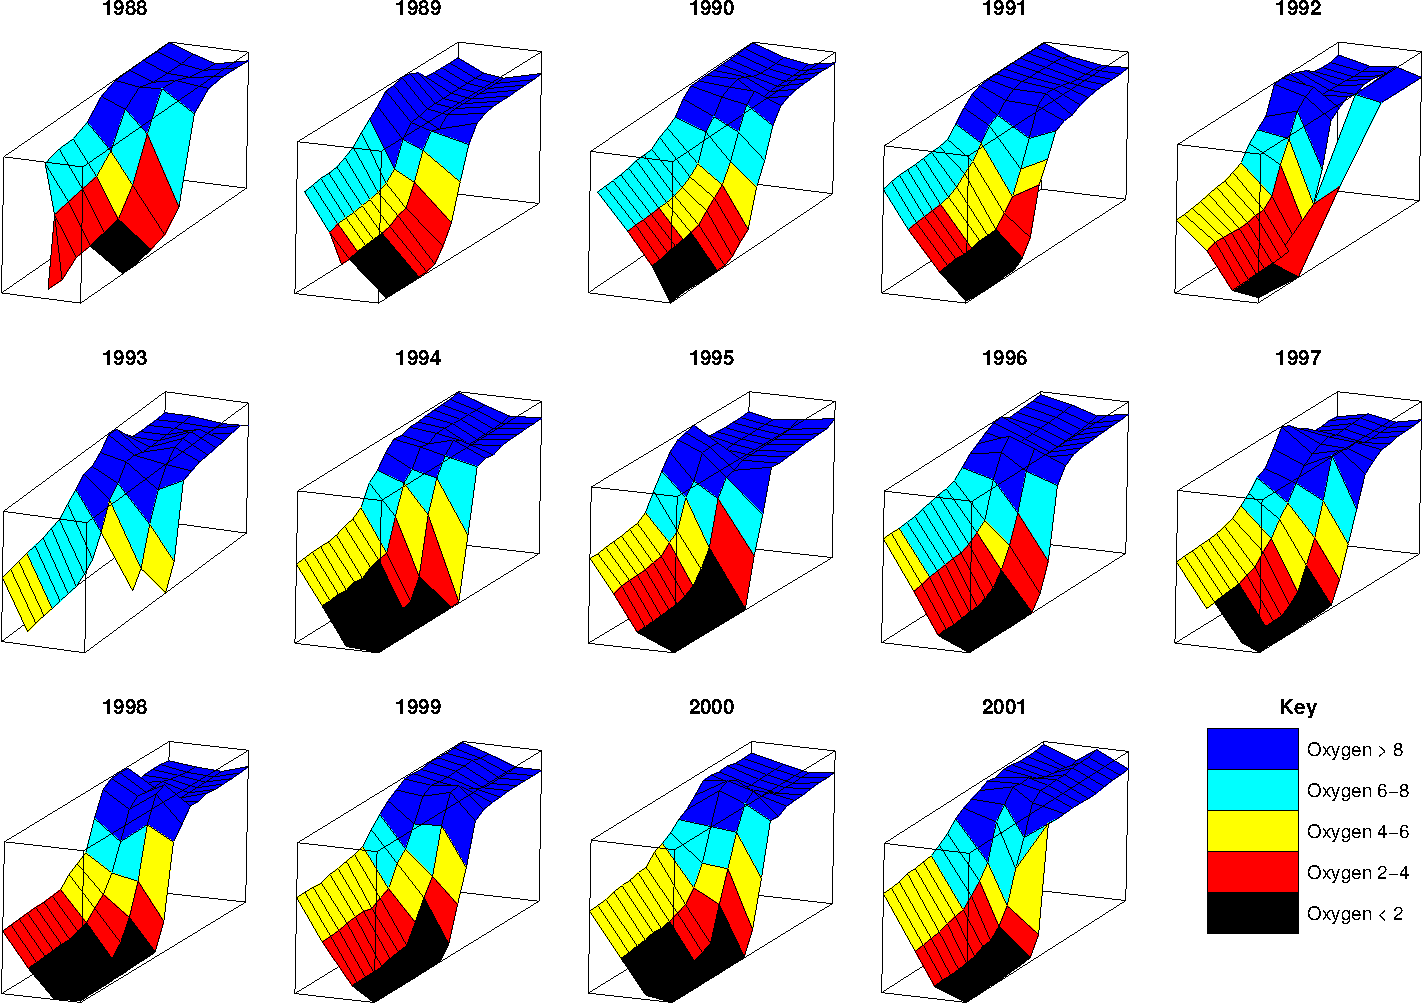
\includegraphics{./figures/do_3D.pdf}}
\end{center}

{\scriptsize While colorful, this figure is impossible to interpret in anything other than very broad terms\\}

\end{frame}


\begin{frame}
\frametitle{Lake Whatcom Oxygen Data}
\framesubtitle{Back to Basics - Simple Scatterplots}

%% copy from LW files
\begin{center}
\hspace*{-5ex}
\resizebox{3in}{!}{
	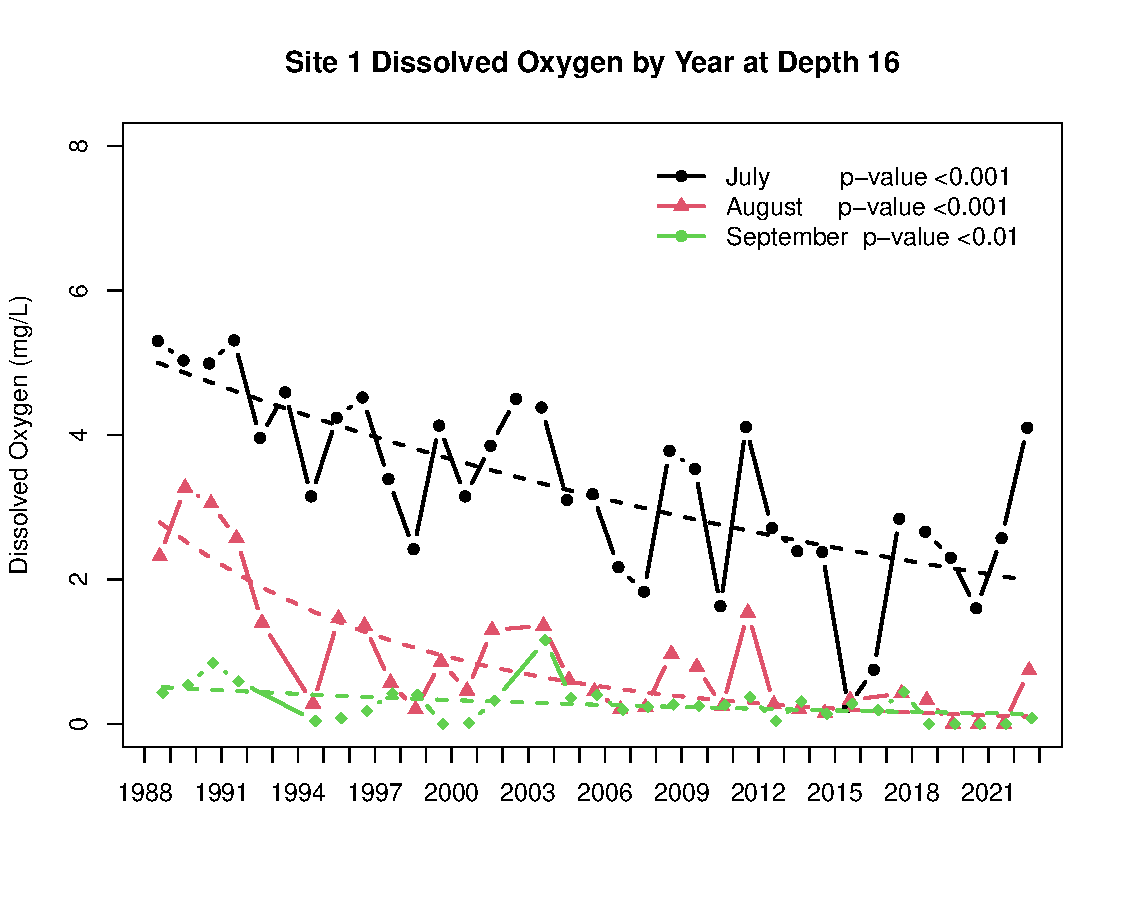
\includegraphics{./figures/Trends-DO-Depth16.pdf}}
\end{center}

\vspace{-0.2in}
       {\scriptsize The important pattern in the two preceding figures is
  that there are different rates of oxygen loss during the summer in
  the deep samples.  Rather than try to show all depths and dates,
  this figure focuses on the changes that are occurring at specific depths and times\\}
\hspace*{2ex}

\end{frame}

\begin{frame}
\frametitle{Lake Whatcom Oxygen Data}
\framesubtitle{Back to Basics - Simple Scatterplots}

%% copy from LW files
\begin{center}
\hspace*{-5ex}
\resizebox{3in}{!}{
	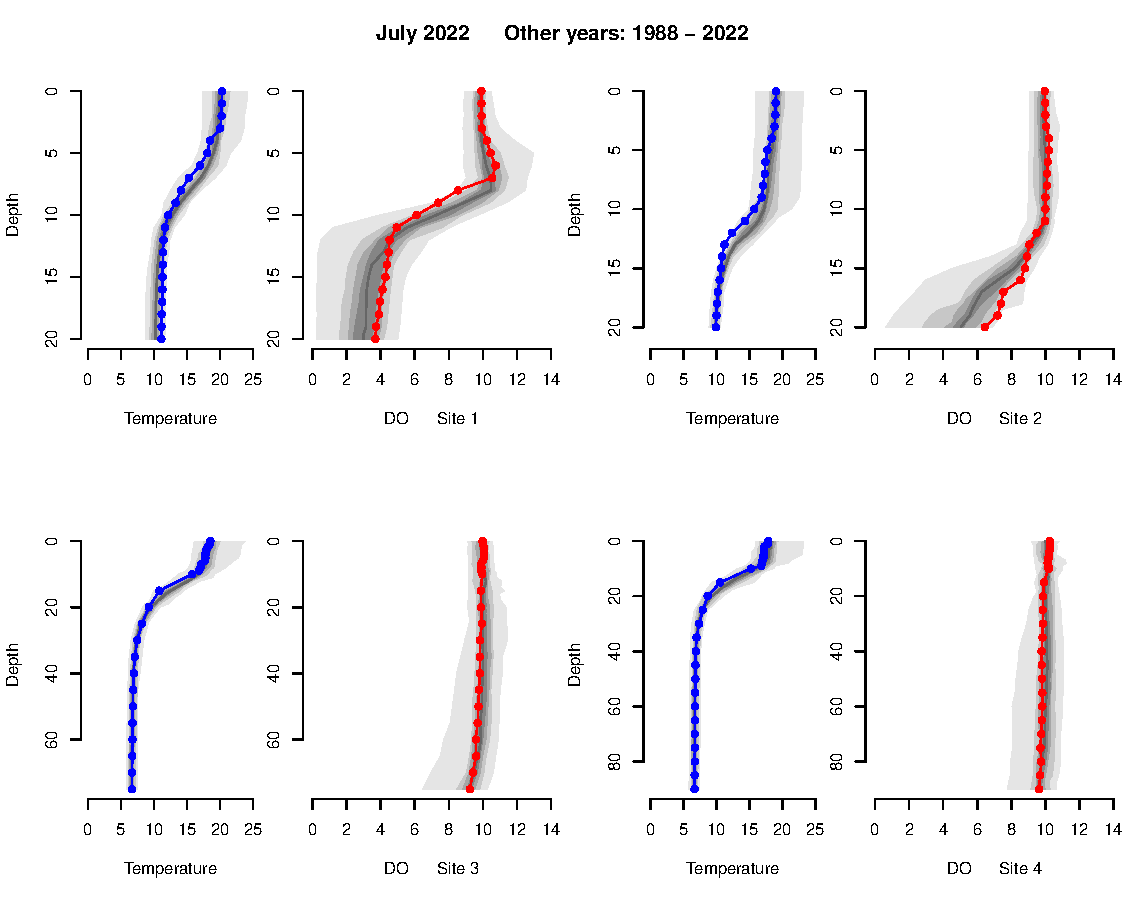
\includegraphics{./figures/HistoricTempDO2022-7.pdf}}
\end{center}

{\scriptsize This figure shows July 2022 temperature and oxygen
  profiles superimposed on polygons shaded to show quartiles on either
  side of the median (historic ranges)\\}
\hspace*{2ex}

\end{frame}



\iwsframe{Correlation and Regression}{The Foundation of Multivariate Analysis}
\bi
\item Both measure {\em monotonic} relationships (see page \pageref{regression1})

\item Regression measures the relationship between an independent
  variable ($x$) and one or more dependent variables ($y_{i}$)

\bi
\item Used to predict (model) unmeasured values of the dependent
  variable(s)
\ei

\item Correlation analysis measures the relationship between two
  variables that are not necessarily functionally dependent

\bi
\item Used to explore patterns in measured variables and to identify
  {\em indicators} that predict responses in other variables
\ei

\item Parametric and nonparametric versions are available for both regression and correlation analysis
\ei

\end{frame}
\iwsframe{Correlation/Regression Summary}{Examples of Monotonic Relationships}
\label{regression1}

\begin{center}
\resizebox{3in}{!}{
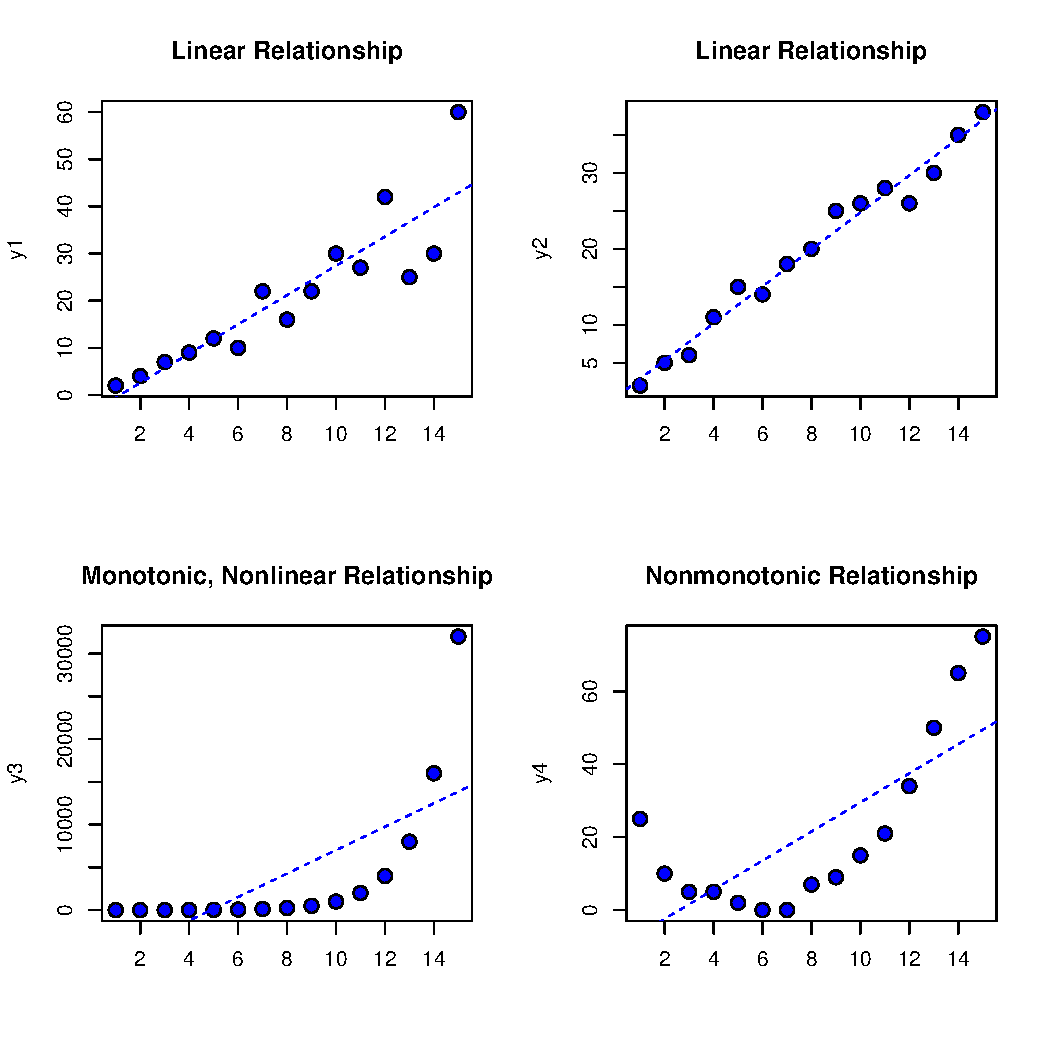
\includegraphics{./figures/monotonic1.pdf}}
\end{center}
\end{frame}

\iwsframe{Correlation/Regression Summary}{Parametric vs.~Nonparametric Correlation Statistics}
\begin{center}
\resizebox{3in}{!}{
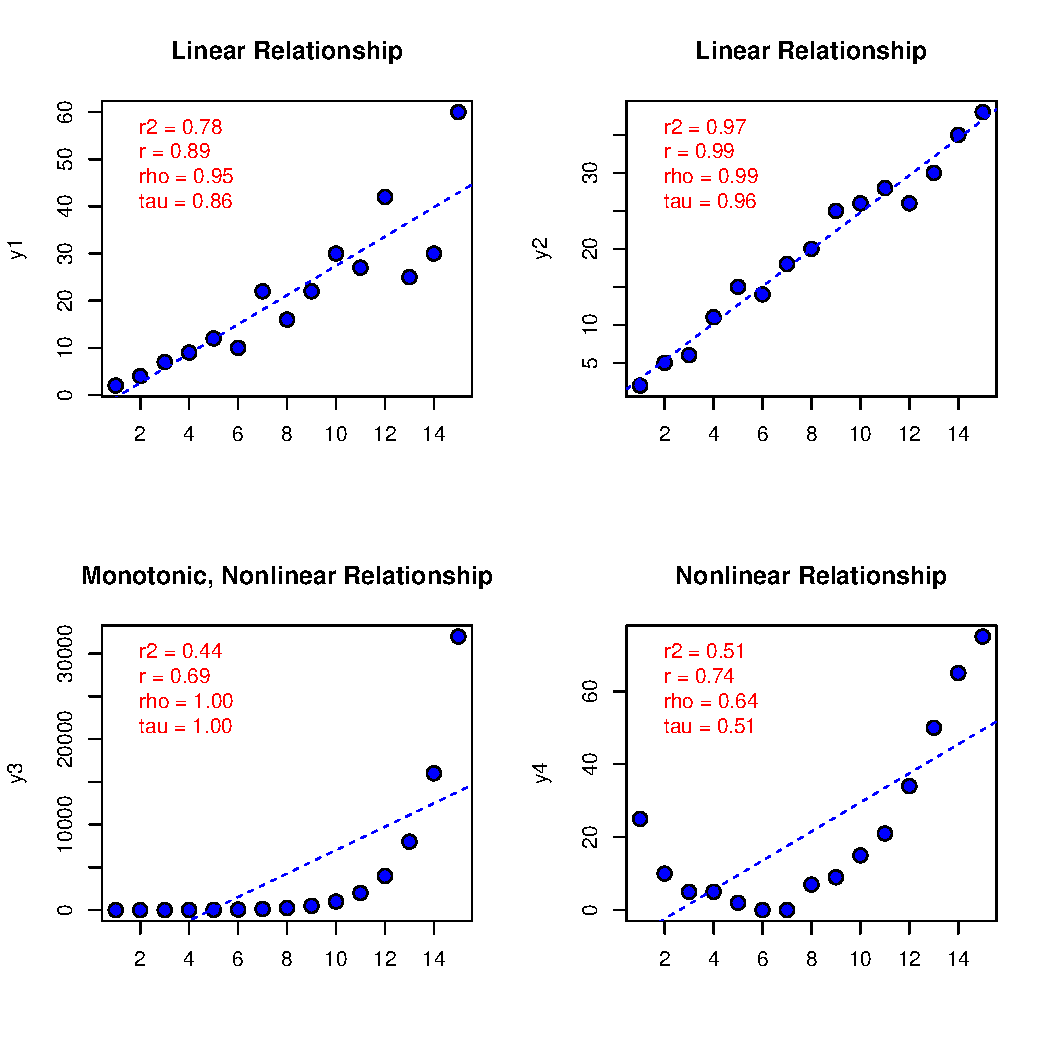
\includegraphics{./figures/monotonic2.pdf}}
\end{center}
\end{frame}


\iwsframe{Correlation Analysis}{Example \#6 - Can Alkalinity Be Used To Predict Chlorophyll?}
\begin{center}
\resizebox{2.5in}{!}{
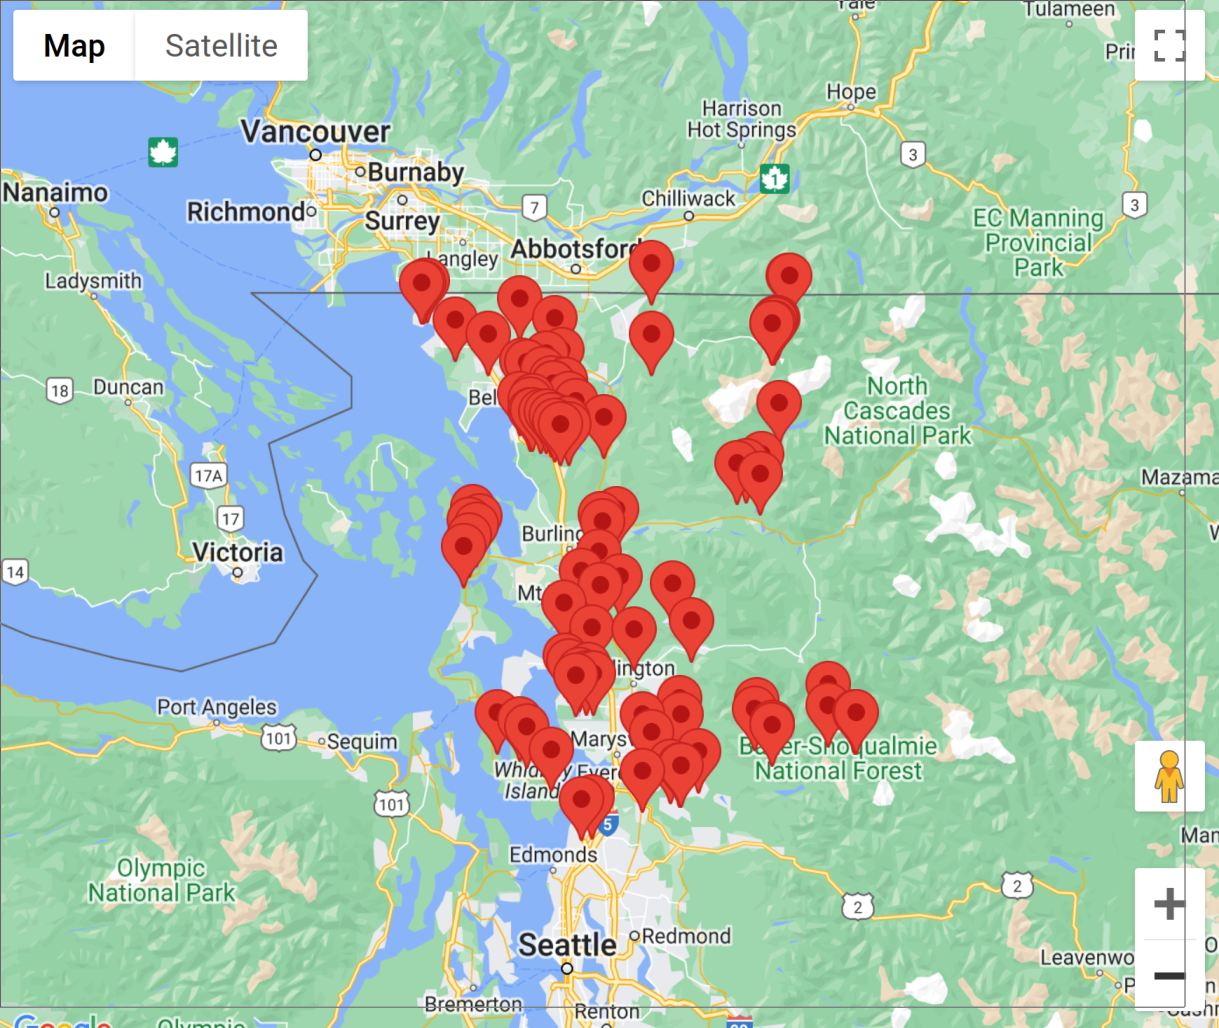
\includegraphics{./figures/small_lakes.pdf}}
\end{center}

{\scriptsize Western Washington University analyzes water samples from 60--70 lakes each the summer. One of the most time consuming analyses is chlorophyll, which is an important indicator of water quality\\}

\end{frame}

\iwsframe{Correlation Analysis}{Example \#6, continued}
\begin{center}
\resizebox{3.5in}{!}{
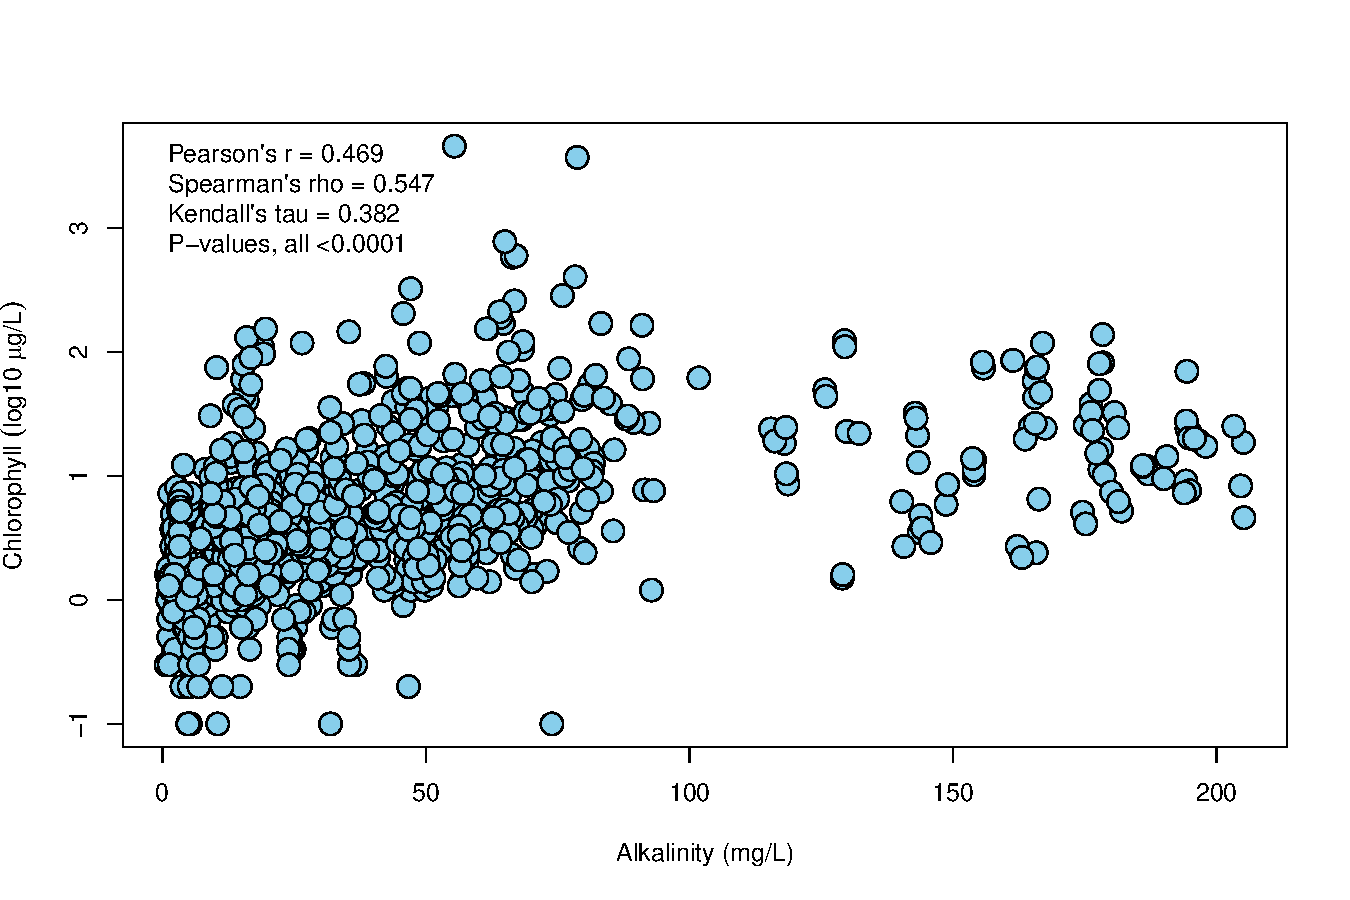
\includegraphics{./figures/correlation1.pdf}}
\end{center}

\vspace*{-2ex}
{\scriptsize Simple correlation analysis shows that there is a monotonic relationship between alkalinity and chlorophyll, which is to be expected from what scientists know about algal photosynthesis.  Can we use alkalinity, which is easier to measure, to estimate chlorophyll in lakes?\\}
\end{frame}


\iwsframe{Regression Analysis}{Example \#6, continued}

\begin{center}
\resizebox{3.5in}{!}{
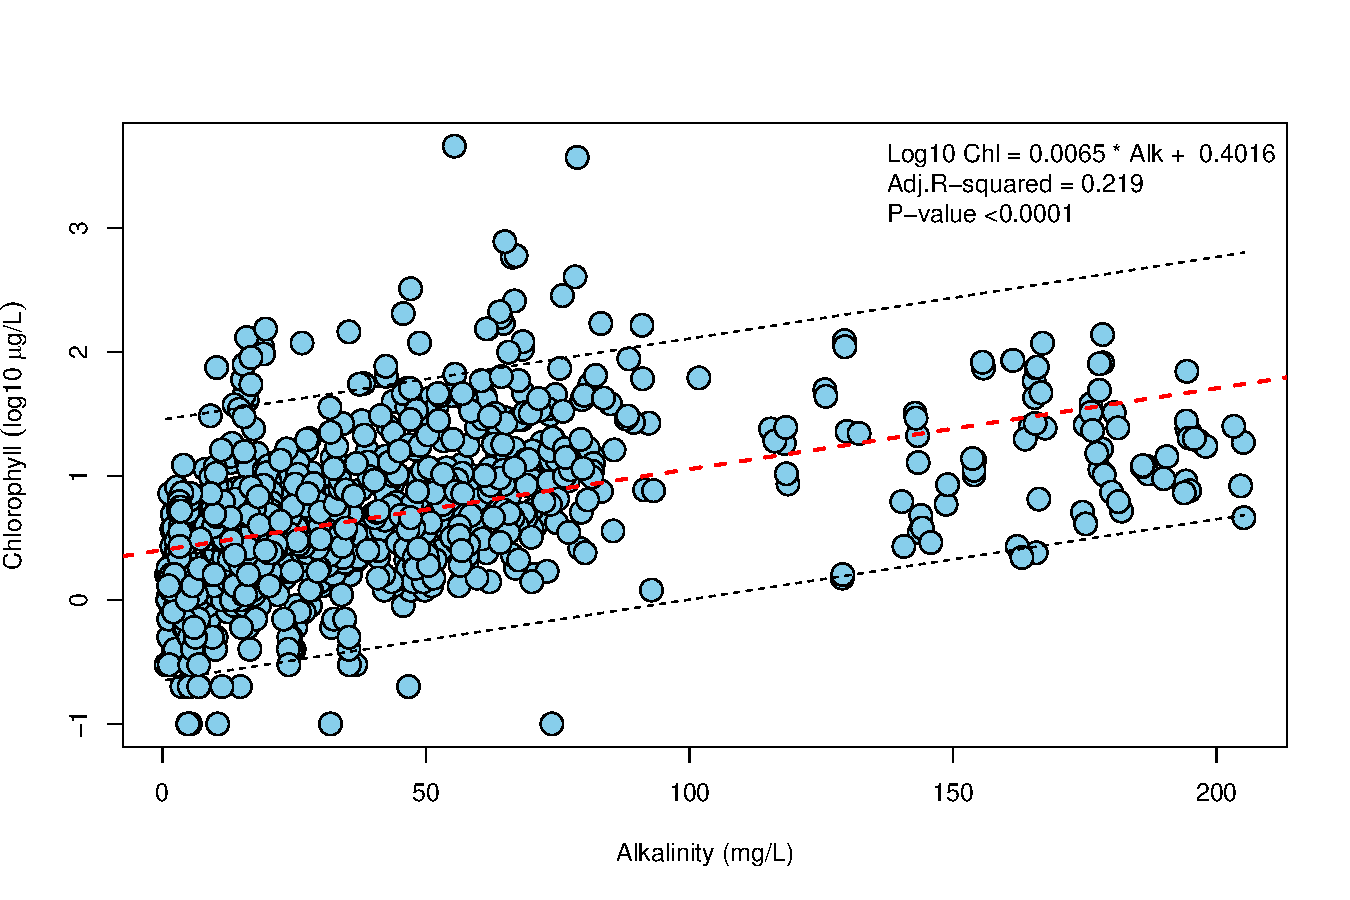
\includegraphics{./figures/regression1.pdf}}
\end{center}

\vspace*{-2ex}

{\scriptsize Regression analysis confirms that you can create a significant linear model\\}

\end{frame}

\iwsframe{Regression Analysis}{Example \#6, continued}

\begin{center}
\resizebox{3.5in}{!}{
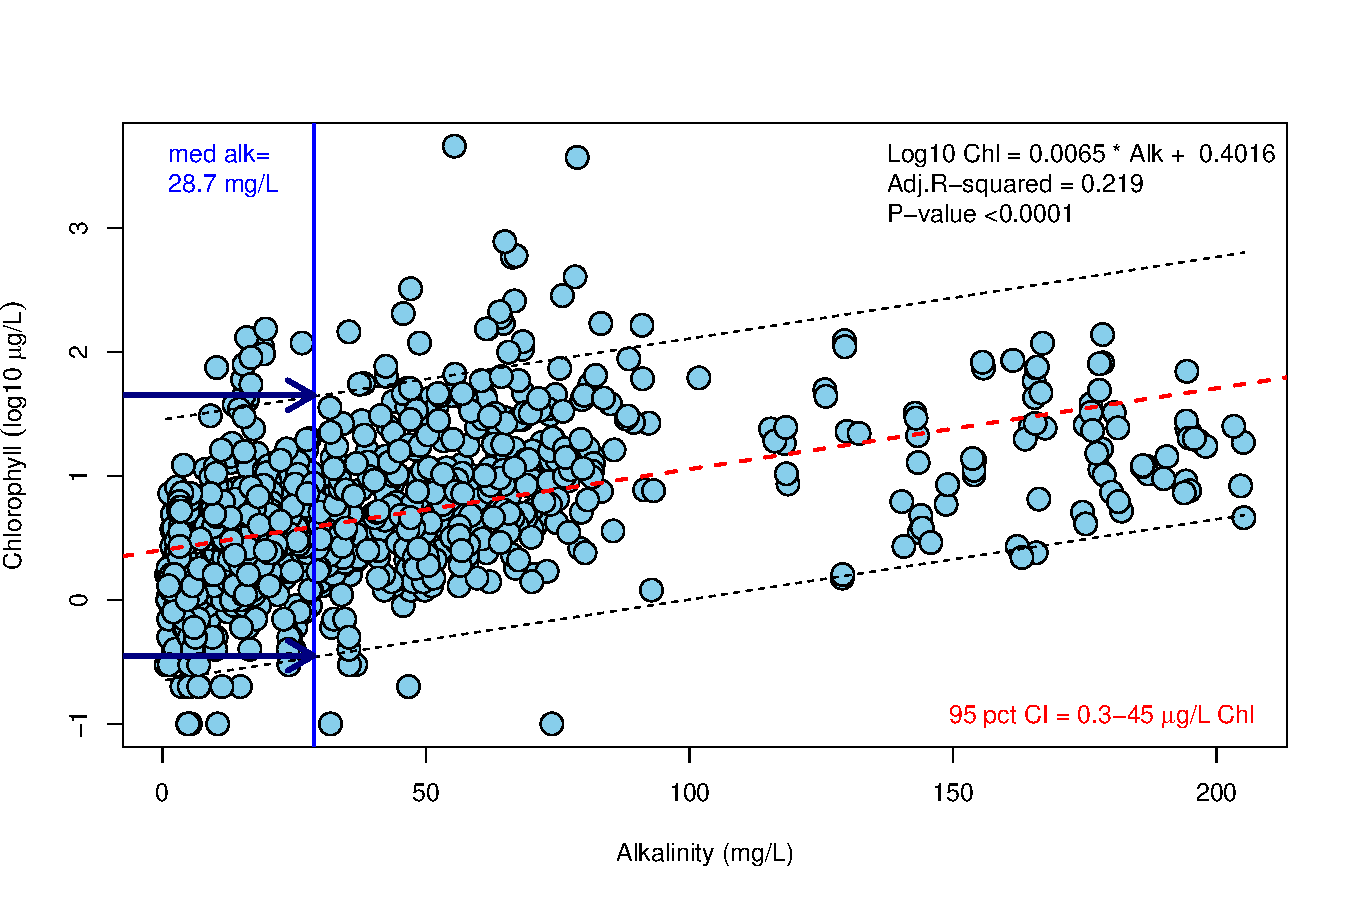
\includegraphics{./figures/regression2.pdf}}
\end{center}

\vspace*{-2ex}

{\scriptsize But the confidence intervals are huge (log scale).  For
  example, at the median alkalinity concentration (28.7 mg/L), the
  95\% CI for chlorophyll is 0.3--45 $\mu$g/L (back transformed from
  the log scale); this is too wide to determine lake water quality\\}
\end{frame}

\begin{frame}
\frametitle{Introduction to Multivariate Analysis}
\framesubtitle{Initial Examination of Multivariate Data}

\bi
{\small
\item Begin by plotting and using simple exploratory tools like correlation
  analysis to look for patterns

{\color{red} The primary purpose of multivariate analysis is data
  simplification $\ldots$ don't use complicated multivariate tests to describe
  simple univariate or bivariate patterns}

\item Check for normality and homoscedasticity  $\ldots$ nearly all
  multivariate methods are parametric 

{\color{red} Heteroscedastic variances are a problem for most multivariate tests}

\item Identify redundant, nonlinear, and random variables $\ldots$ exclude
  those variables if appropriate

{\color{red} Including redundant, nonlinear, and random variables in
  multivariate analysis can obscure patterns in the remaining variables\\}
}
\ei
\end{frame}


\iwsframe{Simple Multivariate Plotting}{Example \#7 - Lake Whatcom Oxygen, Chlorophyll, and Algae Patterns}
\begin{center}
\resizebox{1.75in}{!}{
	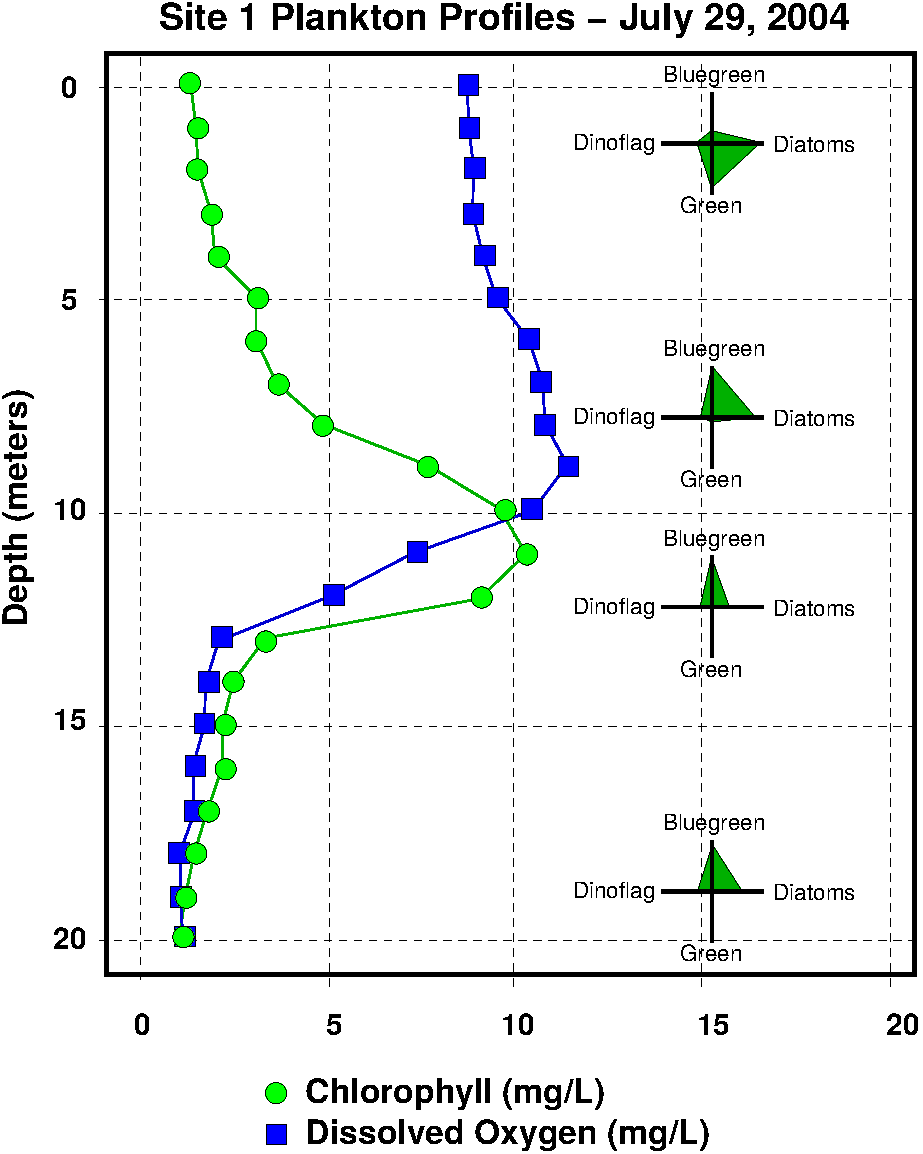
\includegraphics{./figures/kite_LW.pdf}}
\end{center}

{\scriptsize This example shows a scatterplot of oxygen and
  chlorophyll concentrations, plotted by depth, with kite diagrams
  showing the relative abundance of different types of algae\\}
\end{frame}


\iwsframe{Simple Multivariate Plotting}{Example \#8 - July Reservoir Algae and Chlorophyll}
\begin{center}
\resizebox{3in}{!}{
	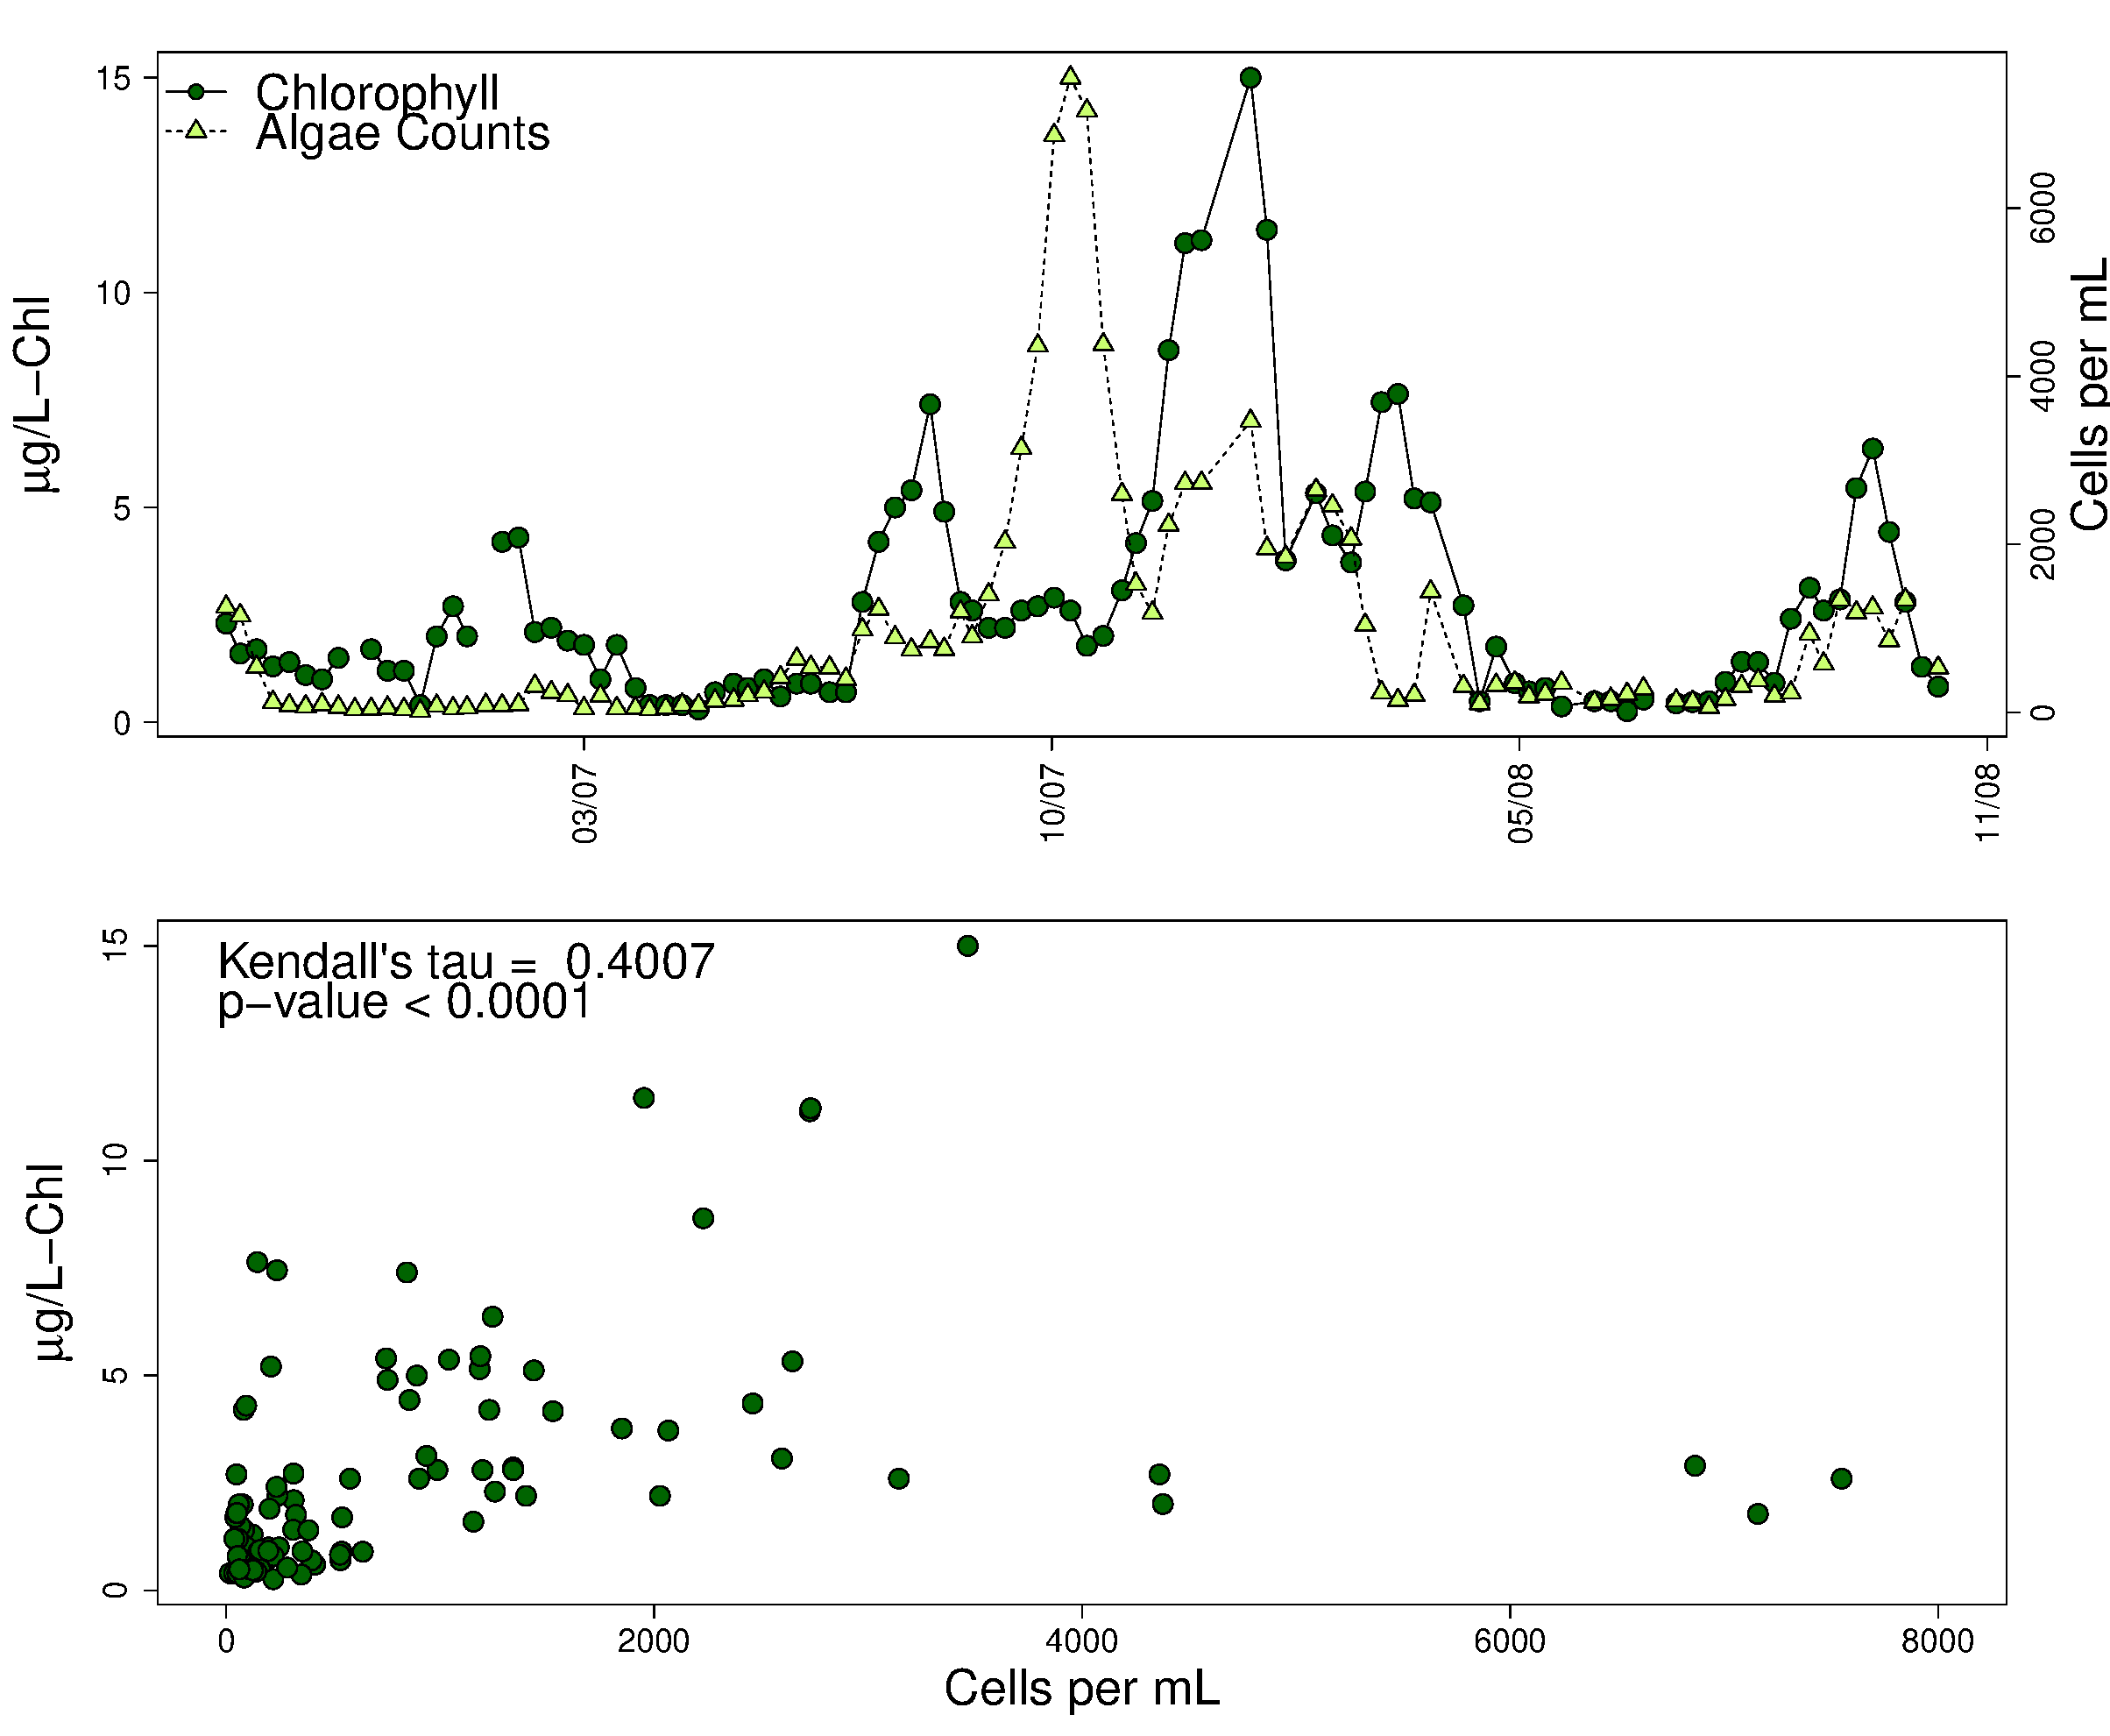
\includegraphics{./figures/algae1a.pdf}}
\end{center}

\vspace*{-0.1in}
{\scriptsize The upper figure is a dual axis plot showing total algae cell
  counts (cells per mL) and chlorophyll concentrations ($\mu$g/L-Chl)
  by date. The lower plot shows the correlation between cells
  counts and chlorophyll (using rank-based Kendall's $\tau$)\\}
\end{frame}

\iwsframe{Multivariate Analysis}{Clustering and Ordination}

{\scriptsize
Two common multivariate patterns include similarity among groups of
samples (clustering) and increasing dissimilarity along a gradient
(ordination)

{\color{blue}Clustering} involves finding similarity among groups of samples:

\begin{center}
\begin{tabular}{|cccccc||cccccc|} \hline
A & B & C & D & E & F	& E & C & A & D & F & B\\ \hline
2 & 3 & 1 & 2 & 1 & 3	& {\bf \color{red}1} & {\bf \color{red}1} & {\bf \color{blue}2} & {\bf \color{blue}2} & {\bf 3} & {\bf 3}\\
2 & 3 & 1 & 2 & 1 & 3	& {\bf \color{red}1} & {\bf \color{red}1} & {\bf \color{blue}2} & {\bf \color{blue}2} & {\bf 3} & {\bf 3}\\
3 & 1 & 2 & 3 & 2 & 1	& {\bf \color{red}2} & {\bf \color{red}2} & {\bf \color{blue}3} & {\bf \color{blue}3} & {\bf 1} & {\bf 1}\\
3 & 1 & 2 & 3 & 2 & 1	& {\bf \color{red}2} & {\bf \color{red}2} & {\bf \color{blue}3} & {\bf \color{blue}3} & {\bf 1} & {\bf 1}\\
1 & 2 & 3 & 1 & 3 & 2	& {\bf \color{red}3} & {\bf \color{red}3} & {\bf \color{blue}1} & {\bf \color{blue}1} & {\bf 2} & {\bf 2}\\
1 & 2 & 3 & 1 & 3 & 2	& {\bf \color{red}3} & {\bf \color{red}3} & {\bf \color{blue}1} & {\bf \color{blue}1} & {\bf 2} & {\bf 2}\\ \hline
\end{tabular}
\end{center}


{\color{blue} Ordination} looks for increasing dissimilarity along a gradient:

\begin{center}
\begin{tabular}{|cccccc||cccccc|} \hline
A & B & C & D & E & F	& E & C & A & D & F & B\\ \hline
3 & 6 & 2 & 4 & 1 & 5	& {\bf \color{red}1} & {\bf \color{blue}2} & {\bf 3} & {\bf \color{magenta} 4} & {\bf 5} & {\bf \color{blue}6}\\
2 & 5 & 1 & 3 & 6 & 4	& {\bf \color{blue}6} & {\bf \color{red}1} & {\bf \color{blue}2} & {\bf 3} & {\bf \color{magenta} 4} & {\bf 5}\\
1 & 4 & 6 & 2 & 5 & 3	& {\bf 5} & {\bf \color{blue}6} & {\bf \color{red}1} & {\bf \color{blue}2} & {\bf 3} & {\bf \color{magenta} 4}\\
6 & 3 & 5 & 1 & 4 & 2	& {\bf \color{magenta} 4} & {\bf 5} & {\bf \color{blue}6} & {\bf \color{red}1} & {\bf \color{blue}2} & {\bf 3}\\
5 & 2 & 4 & 6 & 3 & 1	& {\bf 3} & {\bf \color{magenta} 4} & {\bf 5} & {\bf \color{blue}6} & {\bf \color{red}1} & {\bf \color{blue}2}\\
4 & 1 & 3 & 5 & 2 & 6	& {\bf \color{blue}2} & {\bf 3} & {\bf \color{magenta} 4} & {\bf 5} & {\bf \color{blue}6} & {\bf \color{red}1}\\ \hline
\end{tabular}
\end{center}

}
\end{frame}

\begin{frame}
\frametitle{Multivariate Analysis}
\framesubtitle{Hierarchical vs.~Divisive Clustering}

\bi
{\small
\item Most commonly used technique is {\color{blue}agglomerative,
hierarchical clustering}
	\bi
	\item Each sample (row) containing a set of measurements is
          called a {\color{blue} \em point}
	\item Similarity (distance) is calculated between all points (samples)
	\item The closest (most similar) two points are combined into
          a single joined point
	\item The distances between all remaining points and the new
          joined point are recalculated
	\item The next closest two points are joined, and so on
	\ei
\vspace{2ex}
\item Another common technique is {\color{blue}divisive clustering},
where initial groups are defined, then all clusters are iteratively
regrouped until the distances are minimized
}
\ei 
\end{frame}


\iwsframe{Cluster Analysis}{Can You Test Significance of Cluster Results?}

\bi
\item {\color{blue} Clustering} is a ``blind'' exploratory statistic that
  looks for groups in multivariate data.  The output does not provide
  p-values to confirm the significance of the clusters

\vspace{2ex}

\item You can add an {\color{blue} Association Analysis} to test
  whether the cluster groups are significantly associated with
  specific groups in the data (like {\color{red} \tt Species} in the
  iris data)
\vspace{2ex}
\ei 

\end{frame}


%%%% hierarchical clustering results
\iwsframe{Cluster Analysis}{Example \#9 - Fisher's (Anderson's) Iris Data}

{\small
\begin{center}
\resizebox{1.2in}{!}{
	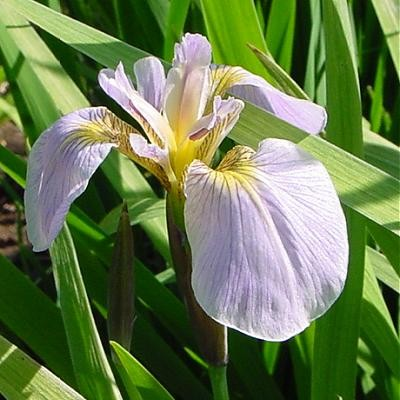
\includegraphics{./figures/Iris-setosa-10_1.jpg}}
\resizebox{1.2in}{!}{
	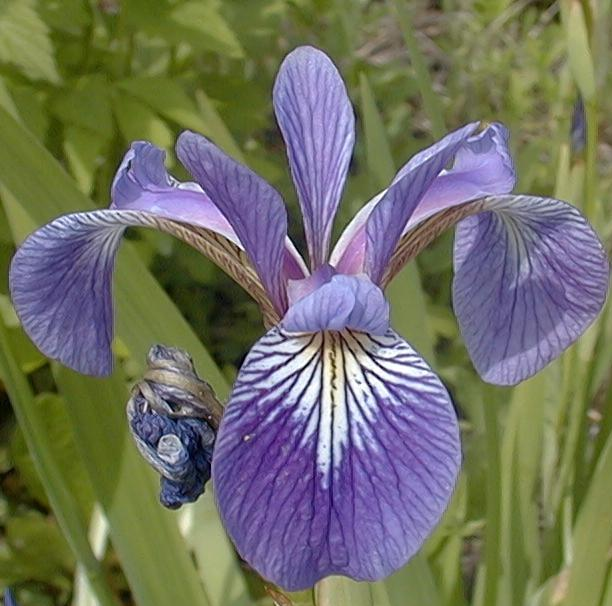
\includegraphics{./figures/Iris-versicolor-21_1.jpg}}
\resizebox{1.2in}{!}{
	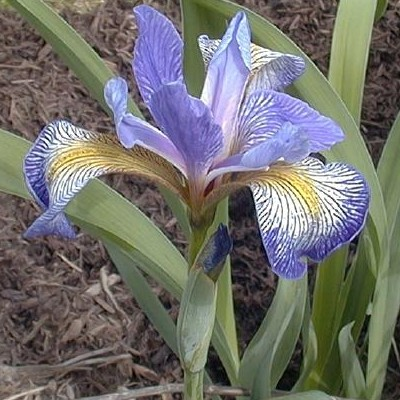
\includegraphics{./figures/Iris-virginica-3_1.jpg}}\\
{\scriptsize 
Photographs by C.~Hensler and D.~Kramb; downloaded with permission from http://www.signa.org
}
\end{center}

\bi
\item {\blue Fisher's Iris data} are widely used to illustrate
  multivariate patterns and evaluate new statistical techniques

\vspace{1ex}
\item The data consist of sepal and petal width and length measurements
from 150 iris flowers representing three species of iris

\vspace{1ex}
\item The iris data are included with the {\tt \red R} ``base
  library'' and can therefore be loaded using the statement {\tt \red
    data(iris)} \ei }
\end{frame}


\begin{frame}[fragile]
\frametitle{Hierarchical Clustering and Association Analysis}
\framesubtitle{Testing Association Between {\color{red} Hierarchical} Clusters and
  Iris Species}

\begin{center}
\resizebox{3.5in}{!}{
	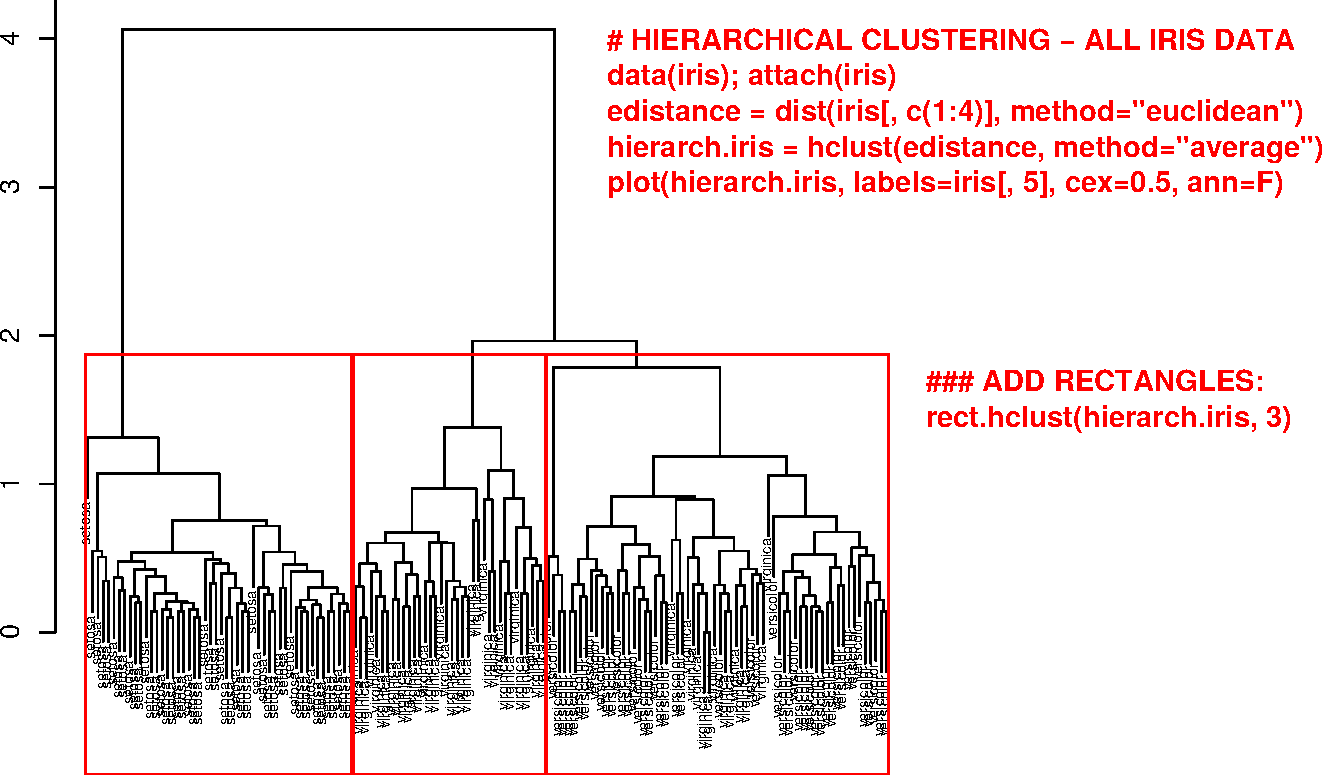
\includegraphics{./figures/cluster3aREV.pdf}}
\end{center}
\end{frame}


\begin{frame}[fragile]
\frametitle{Hierarchical Clustering and Association Analysis}
\framesubtitle{Testing Association Between Hierarchical Clusters and
  Iris Species}

{\scriptsize \color{red}
\verb% irisgroup = cutree(hierarch.iris, 3) # form 3 groups from cluster results%\\
\verb% table(irisgroup, iris$Species)       # show cluster groups vs species%\\
}

\vspace{1ex}

{\scriptsize \color{blue}
\verb% irisgroup setosa versicolor virginica%\\
\verb%         1     50          0         0%\\
\verb%         2      0         50        14%\\
\verb%         3      0          0        36%\\
}

\vspace{2ex}
{\scriptsize \color{red}
\verb% chisq.test(irisgroup, iris$Species)%
}

\vspace{1ex}

{\scriptsize \color{blue}
\verb%        Pearson's Chi-squared test%

\verb% data:  irispart$Species and irisgroup%\\
\verb% X-squared = 234.375, df = 4, p-value < 2.2e-16%\\
}

\vspace{2ex} 

{\scriptsize

This combination of {\color{red} \tt table} and {\color{red} \tt
    chisq.test} is often called {\em \color{blue} Association Analysis}.  We
  are showing the association between the hierarchical clusters and Iris
  Species using a contingency table ({\color{red} \tt table}) and testing the
  significance of the association using {\color{red} \tt chisq.test}

\vspace{2ex}

Hierarchical clustering correctly grouped all {\em setosa} and {\em versicolor}
samples, but misclassified 14 of the {\em virginica} samples (39\%).  The
total misclassification rate was 9.3\% (14 out of 150)\\}

\end{frame}



\begin{frame}[fragile]
\frametitle{Kmeans Clustering and Association Analysis}
\framesubtitle{Testing Association Between {\color{red} Kmeans} Clusters and
  Iris Species}

{\scriptsize \color{red}
\verb% kmeans.iris = kmeans(iris[, c(1:4)], 3)%\\
\verb% table(iris$Species, kmeans.iris$cluster)%\\
}

\vspace{1ex}

{\scriptsize \color{blue}
\verb%             1  2  3%\\
\verb%  setosa     50  0  0%\\
\verb%  versicolor  0 48  2%\\
\verb%  virginica   0 14 36%\\
}

\vspace{2ex}
{\scriptsize \color{red}
\verb%chisq.test(iris$Species, kmeans.iris$cluster)%\\
}

\vspace{1ex}

{\scriptsize \color{blue}
\verb%        Pearson's Chi-squared test%\\

\vspace{1ex}

\verb% data:  iris$Species and kmeans.iris$cluster%\\
\verb% X-squared = 223.5993, df = 4, p-value < 2.2e-16%\\
}

\vspace{2ex} 
{\scriptsize Kmeans clustering correctly clustered {\em setosa}, but placed 2
  of the {\em versicolor} and 14 of the {\em virginica} into the wrong
  groups (10.7\% total misclassification).

\vspace{1ex} 

Because kmeans clustering has an element of uncertainty, repeating the
clustering process can give you different results.  For example, one of my
cluster ``runs'' misclassified 17 {\em setosa} and 4 {\em versicolor} (14\%
misclassification)\\}

\end{frame}



\begin{frame}[fragile]
\frametitle{Kmeans Clustering and Association Analysis}
\framesubtitle{Plotting the Association Analysis Results}

{\scriptsize One of the features of {\color{red} \tt kmeans}
  clustering is that it provides information about which variables
  contribute to cluster separation.  To access that information, type the
  cluster object ({\color{red} \tt kmeans.iris}) and look at {\color{blue} \tt
    Cluster means:\\}
}

\vspace{2ex}
{\scriptsize \color{red}
\verb% kmeans.iris  # review the kmeans cluster features%\\
}

\vspace{1ex}

{\scriptsize \color{blue}
\verb% K-means clustering with 3 clusters of sizes 50, 62, 38%\\

\verb% Cluster means:%\\
\verb%   Sepal.Length Sepal.Width Petal.Length Petal.Width%\\
\verb% 1     5.006000    3.428000     1.462000    0.246000%\\
\verb% 2     5.901613    2.748387     4.393548    1.433871%\\
\verb% 3     6.850000    3.073684     5.742105    2.071053%\\
}

\vspace{2ex}
{\scriptsize
The {\color{blue} \tt Cluster means} are the centers for each variable by
group.  So, for example, the cluster center for petal width in group \#1 is
0.246.  Group \#1 contains all of the {\em Iris setosa} samples, which have
short, narrow petals.  By examining the cluster centers you should be able to
see that petal lengths and widths are good plotting choices for displaying the
results!\\ }

\end{frame}



\begin{frame}[fragile]
\frametitle{Kmeans Clustering and Association Analysis}
\framesubtitle{Plotting the Association Analysis Results}

\begin{center}
\resizebox{2.2in}{!}{
	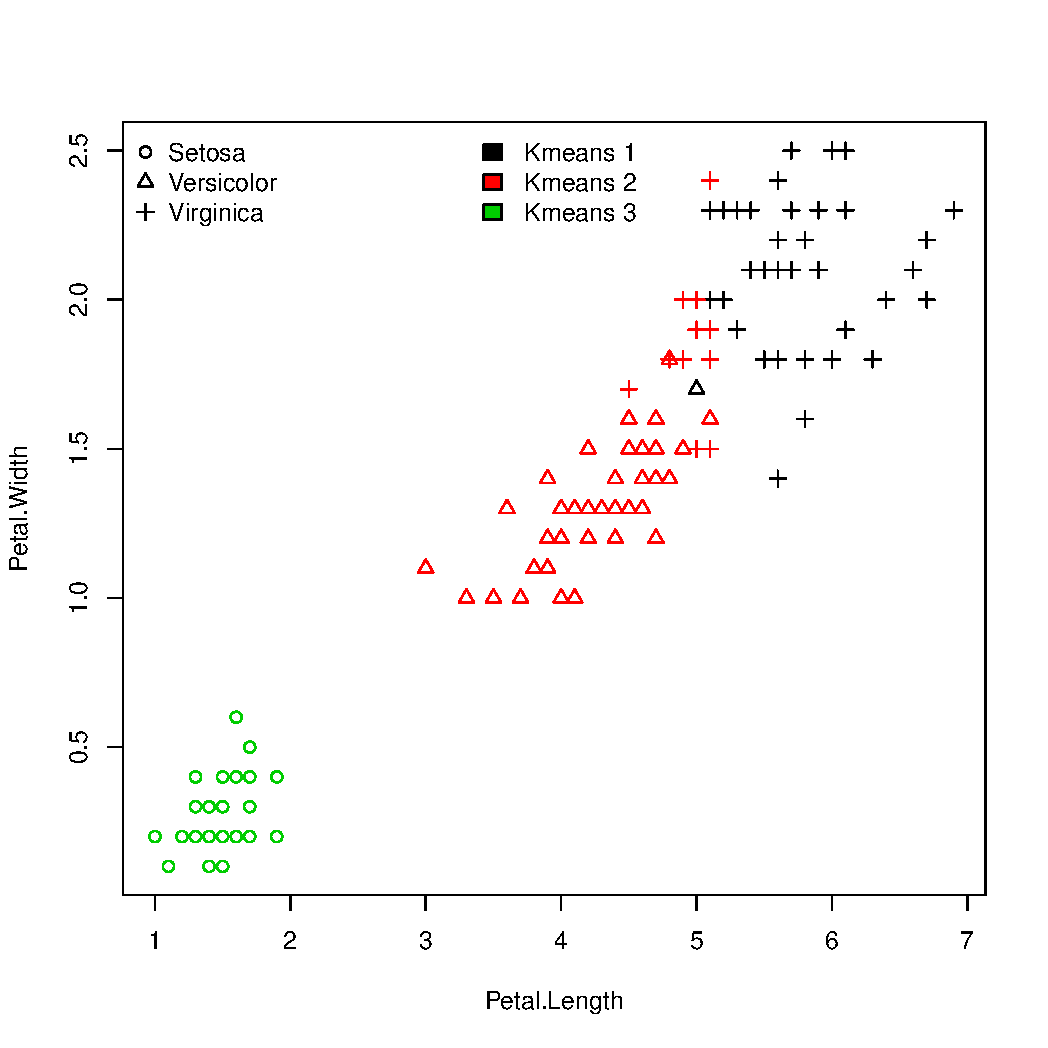
\includegraphics{./figures/cluster3b.pdf}}
\end{center}

\vspace*{-2ex}
{\scriptsize \color{red}
\verb% plot(Petal.Length, Petal.Width, col=kmeans.iris$cluster, pch=unclass(iris$Species))%\\
\verb% legend(x="topleft", c("Setosa", "Versicolor", "Virginica"), pch=c(1,2,3), bty="n")%\\
\verb% legend(x="top", c("Kmeans 1", "Kmeans 2", "Kmeans 3"), fill=c(1,2,3), bty="n")%\\
}

\end{frame}


\begin{frame}
\frametitle{Randomization Testing}
\framesubtitle{Time for a Reality Check!}

\bi
\item {\color{blue} Randomization testing} is an an excellent reality check
  when working with multivariate data
\vspace{2ex}
\item Rather than relying on assumptions about distributions or tables of
  probabilities, you test whether the results for your {\color{magenta}
  nonrandom} data are likely to occur by chance
\vspace{2ex}
\item To create a randomized sample, each variable was sampled in
  random order, then written back into the same column.  As a result,
  sepal lengths were still in column 1, but the values no longer
  lined up with the correct iris species \ei
\end{frame}


\begin{frame}
\frametitle{Randomization Testing}
\framesubtitle{Boxplots Showing the Effect of Randomization on Iris Data}
\begin{center}
\resizebox{3in}{!}{
	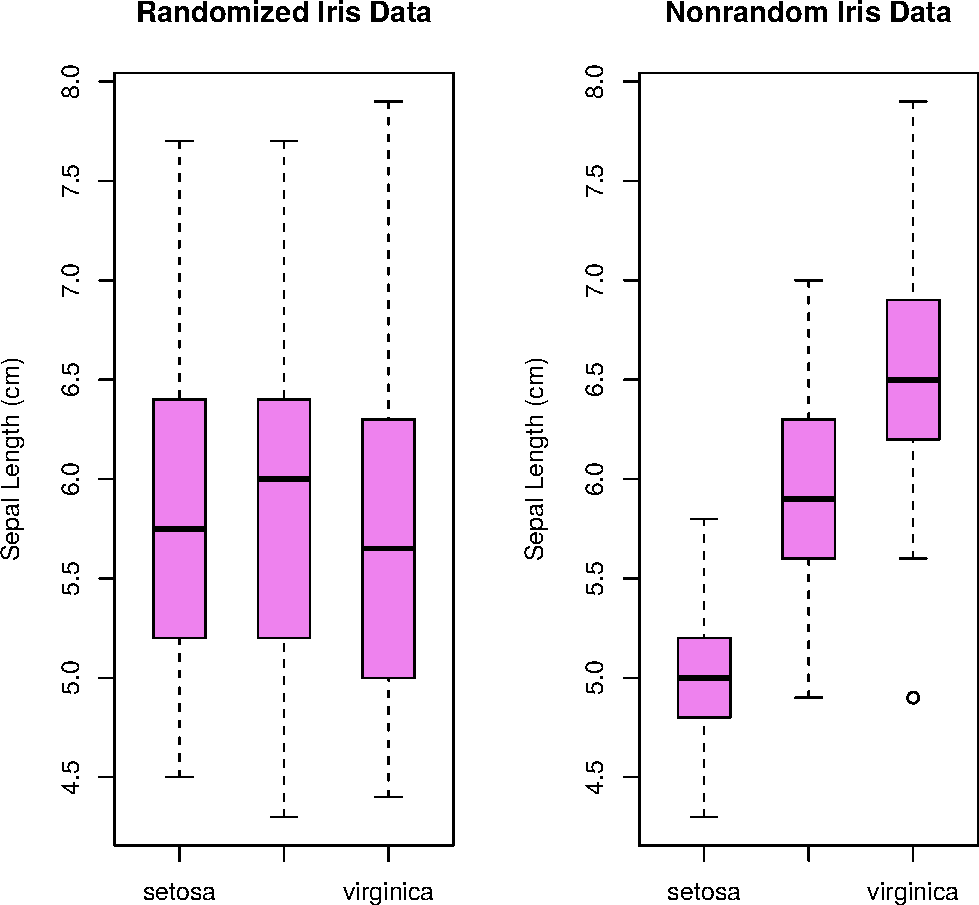
\includegraphics{./figures/random_boxplot.pdf}}
\end{center}
\end{frame}


\begin{frame}
\frametitle{Randomization Testing}
\framesubtitle{Hierarchical Clustering of Randomized Iris Data}
\begin{center}
\resizebox{3in}{!}{
	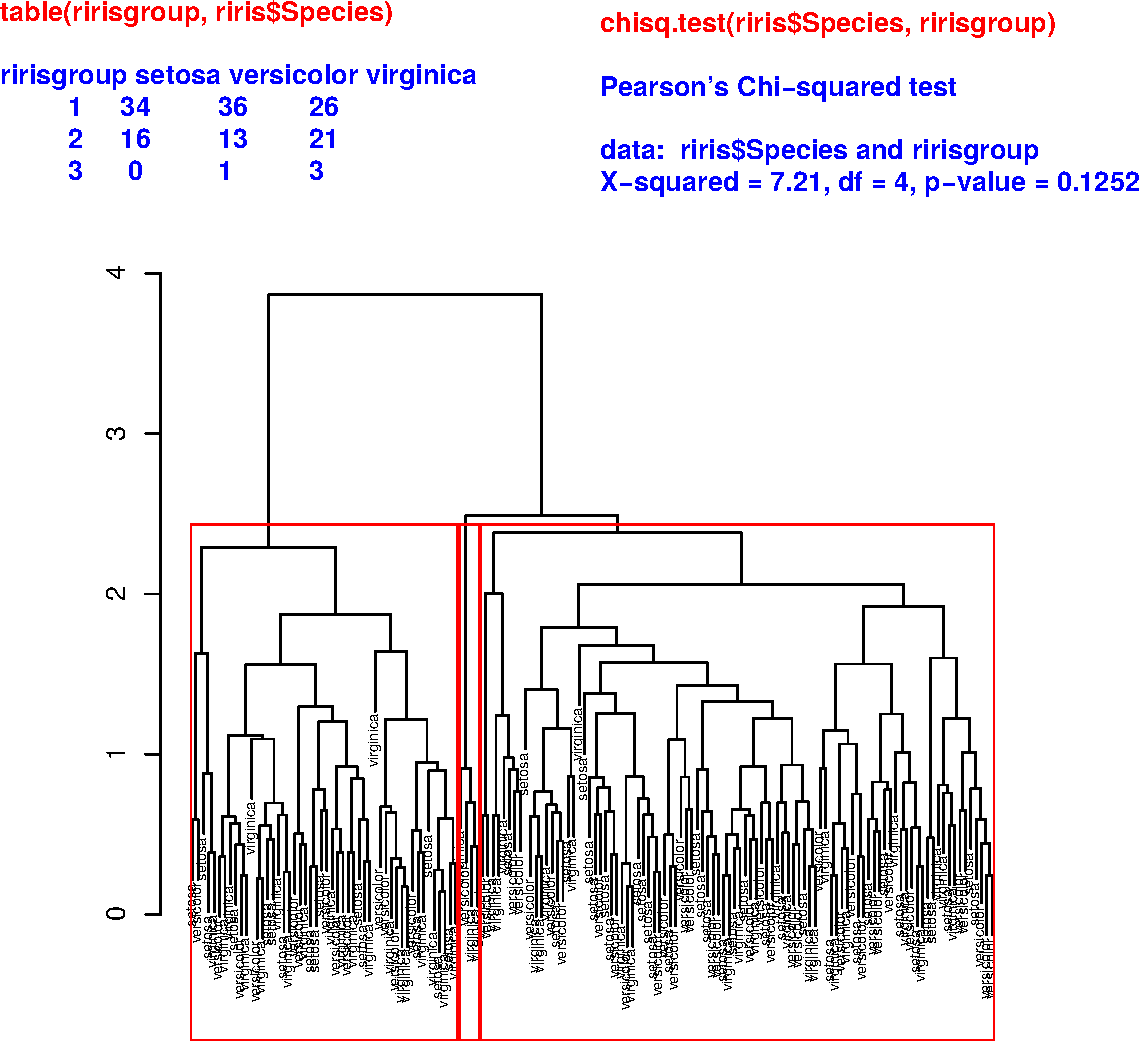
\includegraphics{./figures/cluster3d.pdf}}

\end{center}
\end{frame}


\begin{frame}[fragile]
\frametitle{Randomization Testing}
\framesubtitle{Kmeans Clustering of Randomized Iris Data}
\begin{center}
\resizebox{2.2in}{!}{
	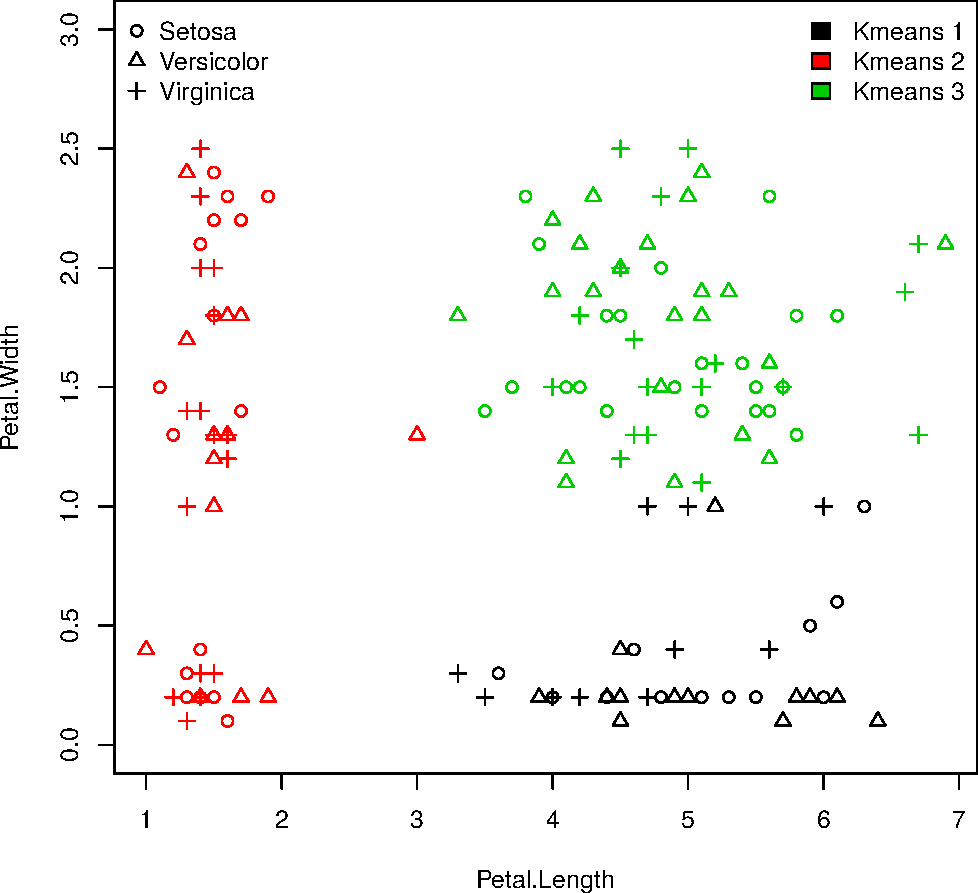
\includegraphics{./figures/cluster3e.pdf}}

\end{center}

\vspace*{-2ex}
{\scriptsize \color{blue}
\hspace{10ex} \verb% ###EDITED ASSOCIATION ANALYSIS OUTPUT:%\\
\hspace{10ex} \verb%              1  2  3%\\
\hspace{10ex} \verb%   setosa     12 16 22%\\
\hspace{10ex} \verb%   versicolor 14 14 22%\\
\hspace{10ex} \verb%   virginica  11 21 18%\\

\vspace{1ex}
\hspace{10ex} \verb% X-squared = 2.4239, df = 4, p-value = 0.6583%\\
}
\end{frame}


\begin{frame}[fragile]
\frametitle{Randomization Testing}
\framesubtitle{Kmeans Clustering and Association Analysis of Randomized Iris Data}

\begin{center}
\begin{tabular}{|c|cc|cc|} \hline
     & \multicolumn{2}{c}{Randomized Data}   & \multicolumn{2}{c|}{Nonrandomized Data} \\
Trial      & X-squared     & p-value  & X-squared & p-value\\ \hline
1          & 2.42          & 0.6583   & 246       & $<$ 2.2e-16\\
2          & 0.36          & 0.9855   & 246       & $<$ 2.2e-16\\
3          & 3.11          & 0.5387   & 255.84    & $<$ 2.2e-16\\
{\color{blue} 4} & {\color{blue} 11.45} & {\color{blue} 0.0219} & {\color{blue} 219.36} & {\color{blue} $<$ 2.2e-16}\\
5          & 4.94          & 0.2935   & 219.36    & $<$ 2.2e-16 \\ \hline

\end{tabular}
\end{center}



{\scriptsize You can increase your confidence in the clustering
  results by comparing repeating the process using different
  randomized data sets.  Here is a comparison using 5 randomized data
  sets; the {\color{red} \tt Welch Two Sample t.test} was used to
  determine whether the X-squared statistics are significantly different\\}

\vspace{1ex}
{\color{red} \scriptsize
\hspace*{10ex} \verb% NR = c(246,246,256,219,219); R = c(2.42,0.36,3.11,11.45,4.94)%\\

\vspace{1ex}
{\color{red} \scriptsize
\hspace*{10ex} \verb% t.test(R, NR, var.equal=F)%\\
}

\vspace{2ex}
{\color{blue} \scriptsize
\hspace*{10ex} \verb% t = -28.527, df = 4.489, p-value = 2.578e-06%\\
}
}

\end{frame}

\begin{frame}[fragile]
\frametitle{Multivariate Analysis}
\framesubtitle{Principal Components Analysis}

\bi
\item There are two basic PCA methods: {\color{red} \tt princomp} and
  {\color{red} \tt prcomp}

   \bi
   \item {\color{red} \tt princomp} ordinates using an eigenvalue matrix
   \item {\color{red} \tt prcomp} is based on a singular value
   decomposition of the data matrix, which is generally preferred over
   {\color{red} \tt princomp}
   \item {\color{red} \tt princomp} and {\color{red} \tt prcomp} will
     often produce identical results (number of principal components = number of variables)
   \item But if there are a large number of variables, {\color{red}
     \tt prcomp} truncates after ``almost all'' of the variance is
     contained in the ordination (number of principal components $\le$
     number of variables) \ei

\item Both default to a covariance matrix (matches S-Plus), but the
  best option is a scaled, centered correlation matrix

\item In both methods, omit variables that are constant (e.g.,
  all zeros)

\ei
\end{frame}


\iwsframe{Principal Components Analysis}{Example \#10 - Fisher's (Anderson's) Iris Data}

{\scriptsize
\color{red} 

\verb%##### PRINCOMP VERSION WITH SCALED/CENTERED CORRELATION MATRIX%\\
\verb%data(iris); attach(iris)%\\
\verb%iris.princomp <- princomp(iris[, c(1:4)], cor=T) #Basic PCA command%\\
\verb%summary(iris.princomp)%\\

\vspace{1ex}
\color{blue}
\verb%Importance of components:%\\
\verb%                          Comp.1    Comp.2     Comp.3      Comp.4%\\
\verb%Standard deviation     1.7083611 0.9560494 0.38308860 0.143926497%\\
\verb%Proportion of Variance 0.7296245 0.2285076 0.03668922 0.005178709%\\
\verb%Cumulative Proportion  0.7296245 0.9581321 0.99482129 1.000000000%\\

\vspace{4ex}
\color{red}
\verb%##### PRCOMP VERSION WITH SCALED/CENTERED CORRELATION MATRIX%\\
\verb%iris.prcomp <- prcomp(iris[, c(1:4)], scale=T, center=T)%\\

\vspace{1ex}
\color{blue}
\verb%summary(iris.prcomp)%\\
\verb%Importance of components:%\\
\verb%                          PC1    PC2     PC3     PC4%\\
\verb%Standard deviation     1.7084 0.9560 0.38309 0.14393%\\
\verb%Proportion of Variance 0.7296 0.2285 0.03669 0.00518%\\
\verb%Cumulative Proportion  0.7296 0.9581 0.99482 1.00000%\\
}
\end{frame}


\iwsframe{Principal Components Analysis}{Principal Components Ordination of Iris Samples}
\begin{center}
\resizebox{4in}{!}{
	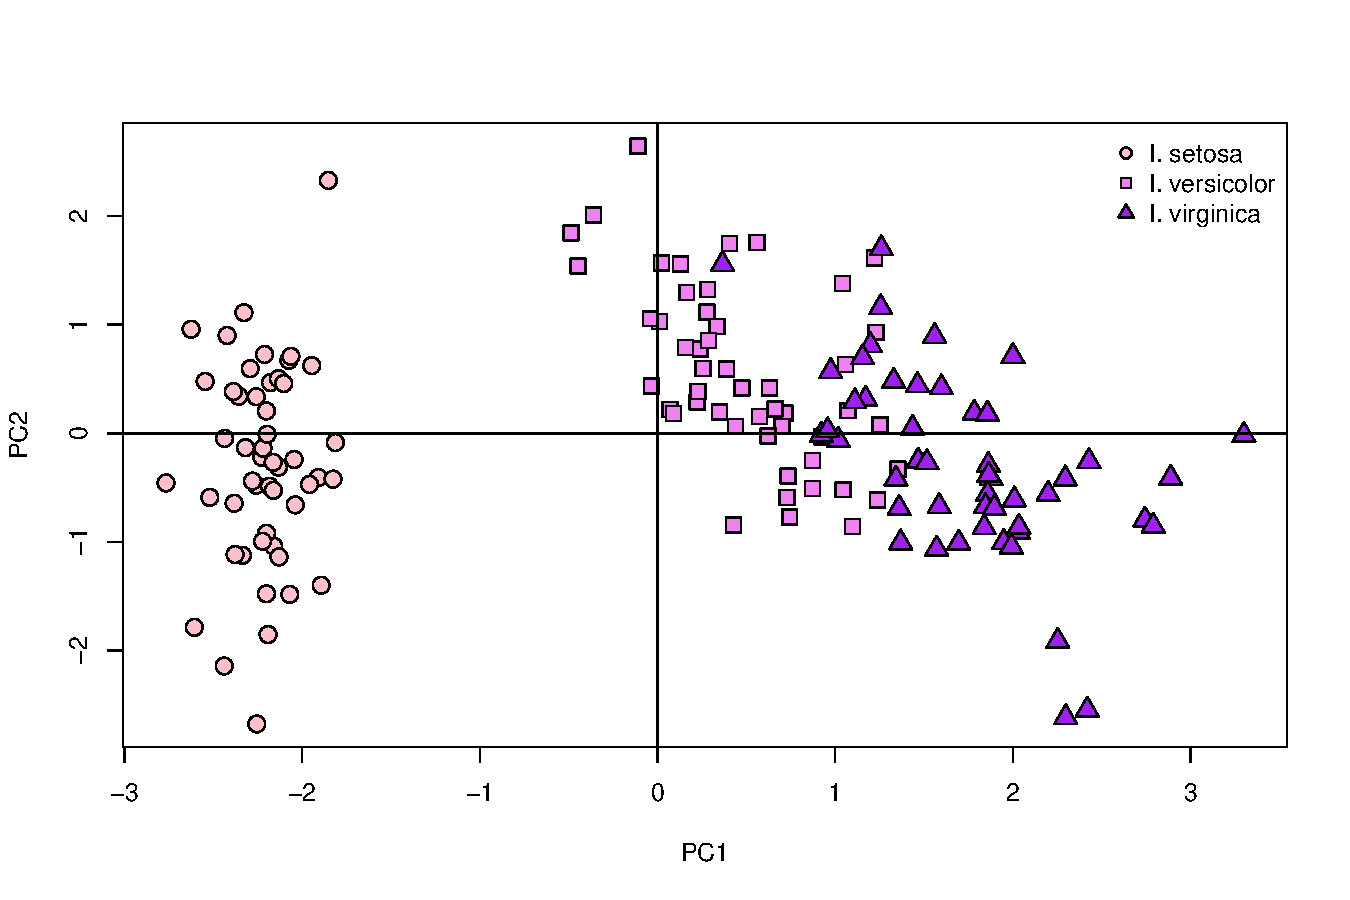
\includegraphics{./figures/irisPRCOMP2.pdf}}
\end{center}
\end{frame}

\iwsframe{Principal Components Analysis}{Biplot Showing Sample and Variable Ordination}
\begin{center}
\resizebox{3.75in}{!}{
  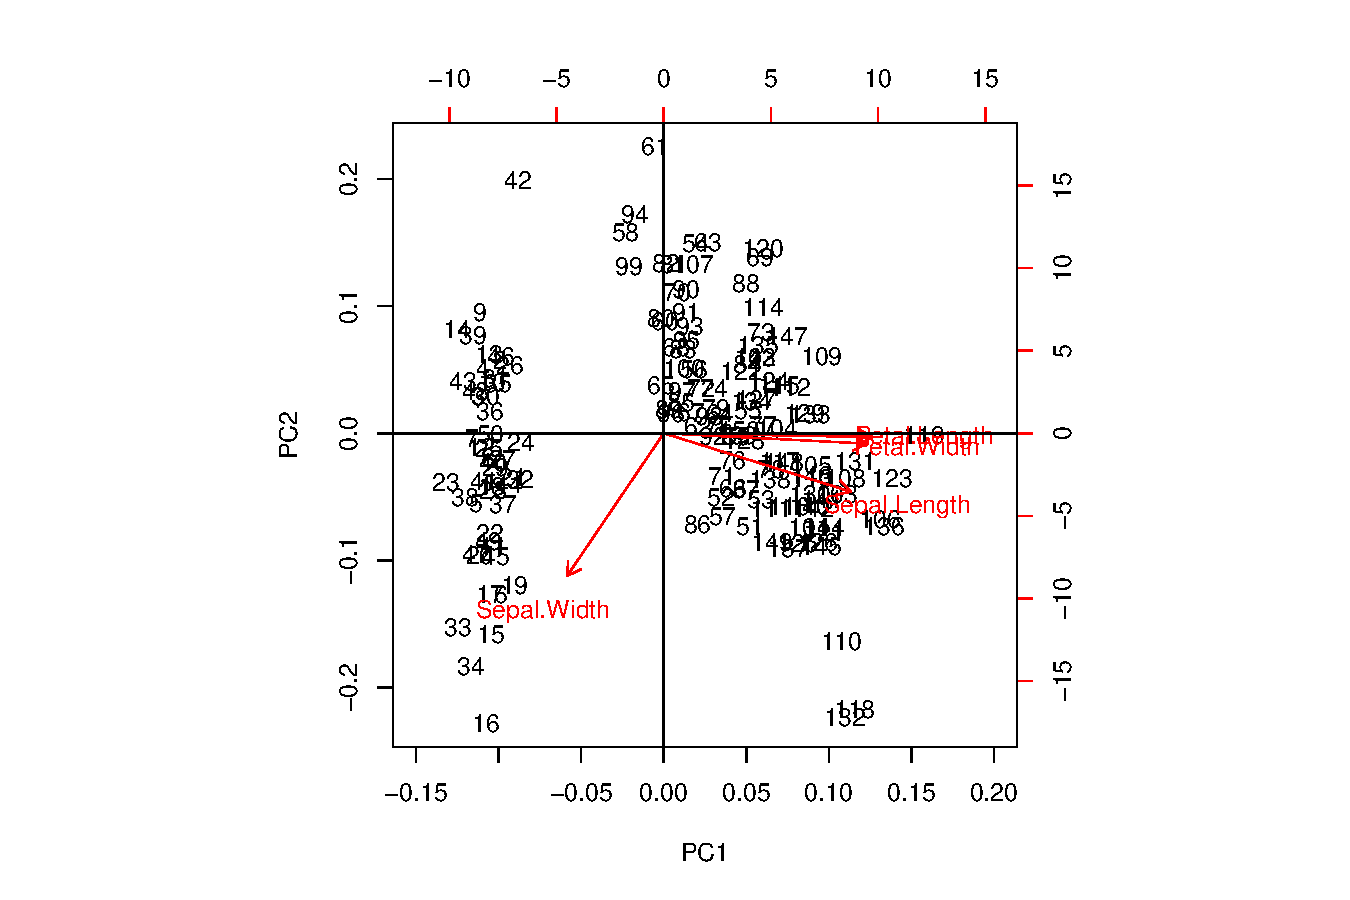
\includegraphics{./figures/irisbiplot.pdf}}
\end{center}

\vspace*{-2ex}

{\scriptsize One PCA goal is variable reduction.  Note how petal
  length/width and sepal length ordinate together on PC1. We could separate the {\em Iris setosa} samples using
  only one variable\\}
\end{frame}



\iwsframe{Principal Components Analysis}{Variable Reduction Features}
\bi
\item Another PCA goal is to find the smallest number of
  components needed to ordinate the samples

\item The simplest approach is to look at the variance plot and see
  where it falls off sharply

\item Another method is to use Kaiser's criterion (default in SPSS) -
  select components with variance $\ge$1$^{\dag}$

%pca.sd = c(1.7083611,0.9560494,0.38308860,0.143926497)
%pca.sd^2

{\footnotesize
\color{blue}
\verb%                          Comp.1    Comp.2     Comp.3      Comp.4%\\
\verb%Standard deviation     1.7083611 0.9560494 0.38308860 0.143926497%\\
\vspace{1ex}

\color{black}
\verb%Variance (sd^2)        2.92      0.91      0.15       0.02      %

}

\vspace{4ex}
{\scriptsize $^{\dag}$Kaiser, H. F.  1960.  {\em The application of electronic
  computers to factor analysis.}  Ed.~and Psychol.~Measurement, 20:
141-151\\}

\ei
\end{frame}



\iwsframe{Principal Components Analysis}{Variance Plot - Note Importance of PC1}
\begin{center}
\resizebox{3in}{!}{
	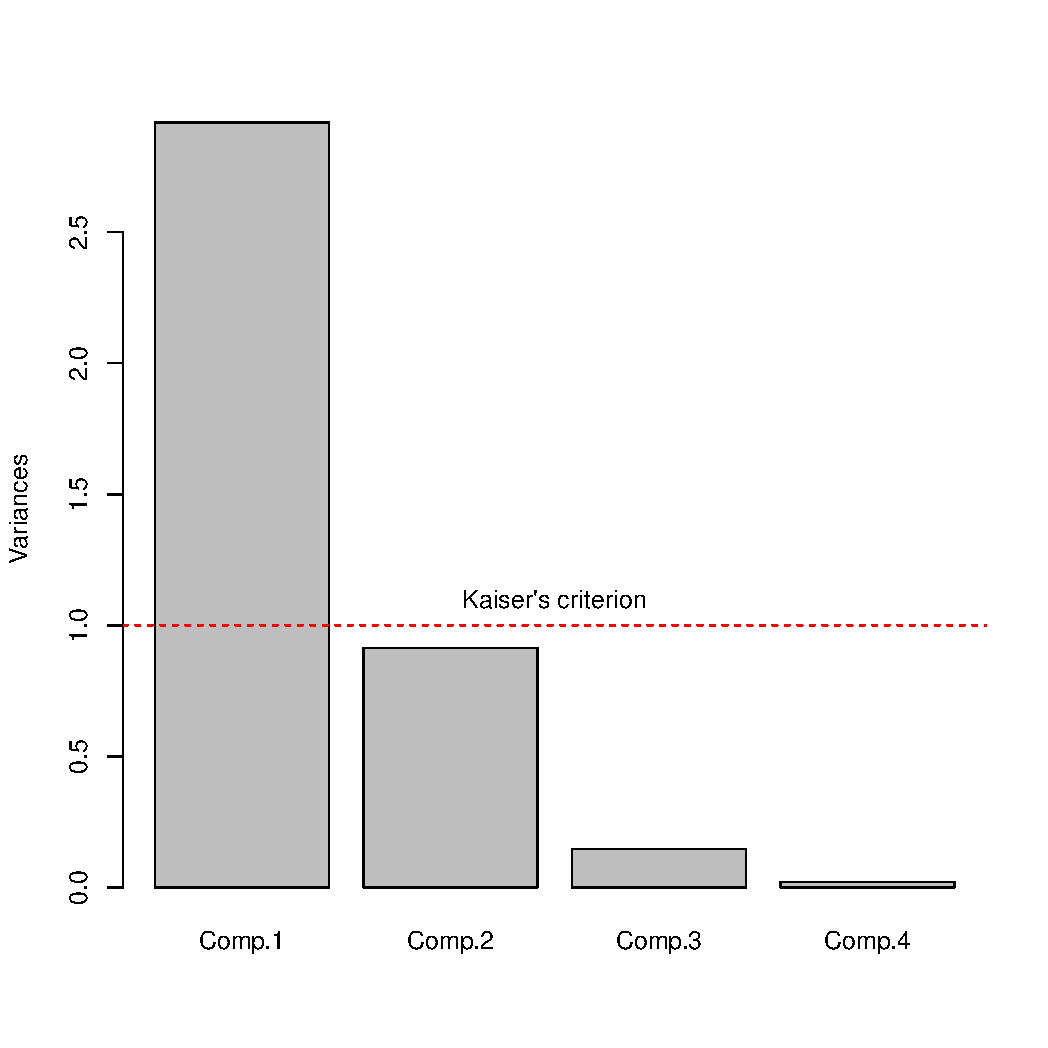
\includegraphics{./figures/irisvariances2.pdf}}
\end{center}
\end{frame}

\iwsframe{Principal Components Analysis}{Using a Trained PCA to Ordinate New Data}
\begin{center}
\resizebox{2.5in}{!}{
	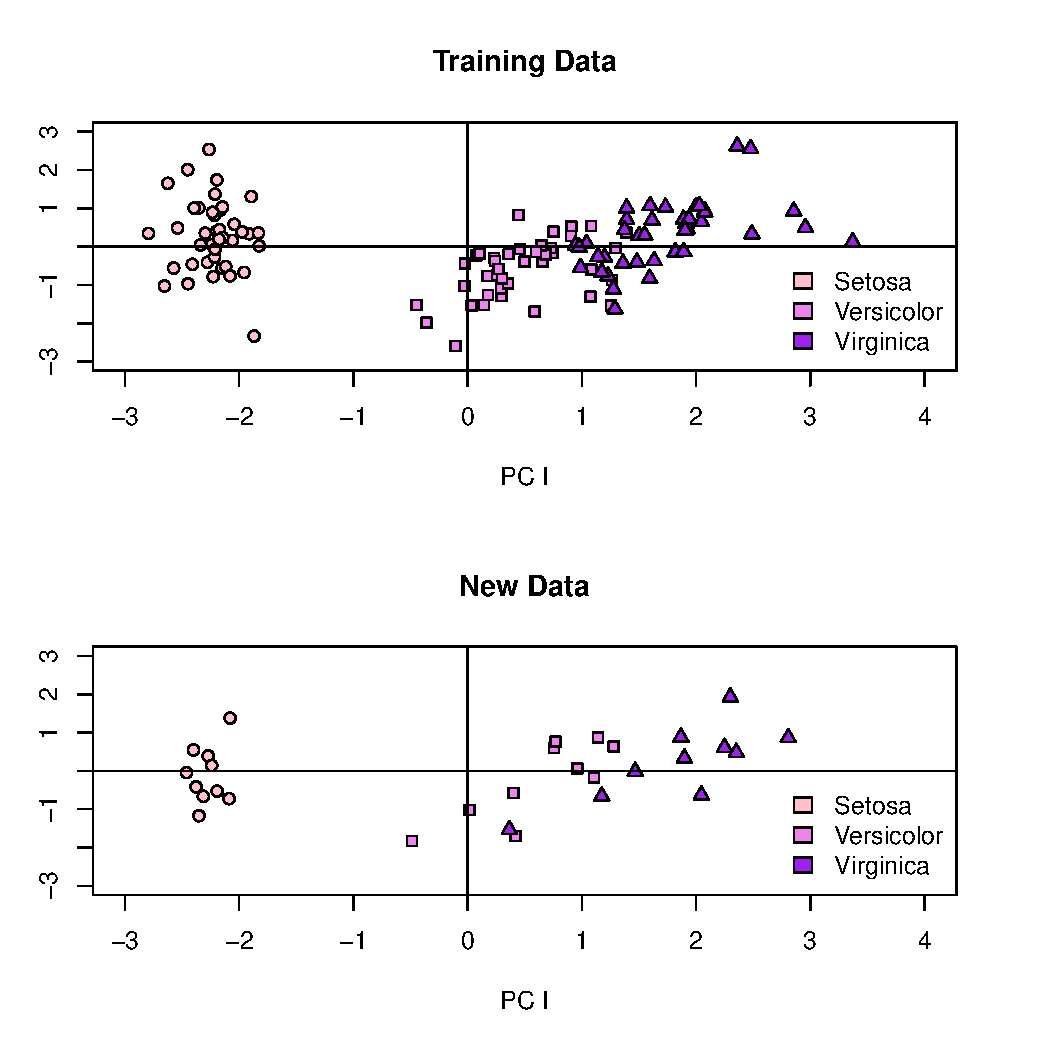
\includegraphics{./figures/irisPRCOMPtrained.pdf}}
\end{center}

\vspace*{-3ex} {\scriptsize A third goal is to use a training set to
  ordinate new data.  This example builds the model using all but the
  first 10 rows for each iris species, then uses the PCA results to ordinate the ``new'' data\\ }
\end{frame}


\iwsframe{Multivariate Analysis}{Clustering on Principal Components}

\begin{itemize}
\item Many multivariate methods default to using all variables in a data set

  \bi
  \item In an earlier slide I mentioned that a common data set problem
    is that not all the measured parameters will show an effect
  \item In data sets with only a few variables, you can make reasonable
    decisions about which variables to omit, but this is not feasible
    for large data sets and can lead to questions about your selection
    criteria \ei
    
\item Alternatively, we can use the variable and component reduction features of PCA to improve
  clustering results without making (potentially) arbitrary selection choices
\end{itemize}
\end{frame}


\begin{frame}[fragile]
\frametitle{Clustering on Principal Components}
\framesubtitle{Example \#11, Effects of Triclosan on Sediment Biota}

{\footnotesize
\begin{itemize}
\item This example is based on data published by Chariton, et
  al.~(2014), following the approach described by Ben-Hur and Guyon
  (2003).

\vspace{1ex}
\item The data are from a sediment toxicity test to determine the
  effects of triclosan, a commonly used antibiotic/antifungal
  compound, on sediment biota.

\vspace{1ex}
\item The biota were identified using molecular markers that
  identified presence or absence of $>$850 unique sediment
  organisms, listed by {\color{blue} \em operational taxonomic
    units} (OTUs) rather than genus and species.  The sediment samples
  contained zero, low, or high concentrations of the toxicant
  (triclosan),

\vspace{1ex}
\item Using OTUs represents an alternative to traditional taxonomic
  assessment because the sediment organisms don't have to
  be sorted, identified, and enumerated to measure biological
  diversity (tedious process!)\\
\end{itemize}
}
\end{frame}


\begin{frame}[fragile]
\frametitle{Clustering on Principal Components}
\framesubtitle{Preliminary Data Decisions}

{\footnotesize

\begin{itemize}
\item The original data file contained presence/absence results for 858 OTUs
  for three treatments (control, low, high) with six replicates per
  treatment.  As a result, the entire file had only 18 rows.

\vspace{1ex}
\item Nine of the OTUs had identical values for all 18 samples
  (variance = zero).  These measurements were excluded from the
  analysis, leaving a data set containing 18 samples and 849 variables

\vspace{1ex}
\item The data were analyzed using PCA based on a singular value
  decomposition of scaled, centered data matrix ({\color{red} \tt
    prcomp}). 

\vspace{1ex}
\item Using this type of PCA has several advantages over
  eigenvector-based PCA, including the ability truncate components if
  the remaining variance approaches zero. In this case, the PCA
  truncated at 18 components (residual variance $<$3.3e-15) rather
  than forcing the use of all 849 components\\
\end{itemize}
}
\end{frame}

\begin{frame}[fragile]
\frametitle{Clustering on Principal Components}
\framesubtitle{Step 1:  Creating New Variables from Component Scores}

{\footnotesize The {\color{red} \tt prcomp} program was used on the
  entire data set (columns 4:852; excluding group,
  treatment, replicate).  The summary function shows that virtually
  all variability can be explained using the first 18 principal
  components (out of 849)\\}

\vspace{2ex}
{\color{blue} \scriptsize
\verb%Importance of components:%\\
\verb%                          PC1   PC2     PC3     PC4    PC5     PC6     PC7%\\
\verb%Standard deviation     10.221 9.880 8.77070 8.08297 7.7312 7.28034 7.03630%\\
\verb%Proportion of Variance  0.123 0.115 0.09061 0.07695 0.0704 0.06243 0.05832%\\
\verb%Cumulative Proportion   0.123 0.238 0.32863 0.40559 0.4760 0.53842 0.59673%\\
\verb% %\\
\verb%                           PC8     PC9    PC10   PC11    PC12    PC13    PC14%\\
\verb%Standard deviation     6.75020 6.71040 6.52041 6.3837 6.27286 5.86208 5.52219%\\
\verb%Proportion of Variance 0.05367 0.05304 0.05008 0.0480 0.04635 0.04048 0.03592%\\
\verb%Cumulative Proportion  0.65040 0.70344 0.75352 0.8015 0.84786 0.88834 0.92426%\\
\verb% %\\
\verb%                          PC15    PC16    PC17      PC18%\\
\verb%Standard deviation     5.05834 4.56602 4.22722 3.321e-15%\\
\verb%Proportion of Variance 0.03014 0.02456 0.02105 0.000e+00%\\
\verb%Cumulative Proportion  0.95440 0.97895 1.00000 1.000e+00%\\
}

\end{frame}


\begin{frame}
\frametitle{Clustering on Principal Components}
\framesubtitle{Variance Plot for First 10 Components}

\begin{center}
\resizebox{2.5in}{!}{
	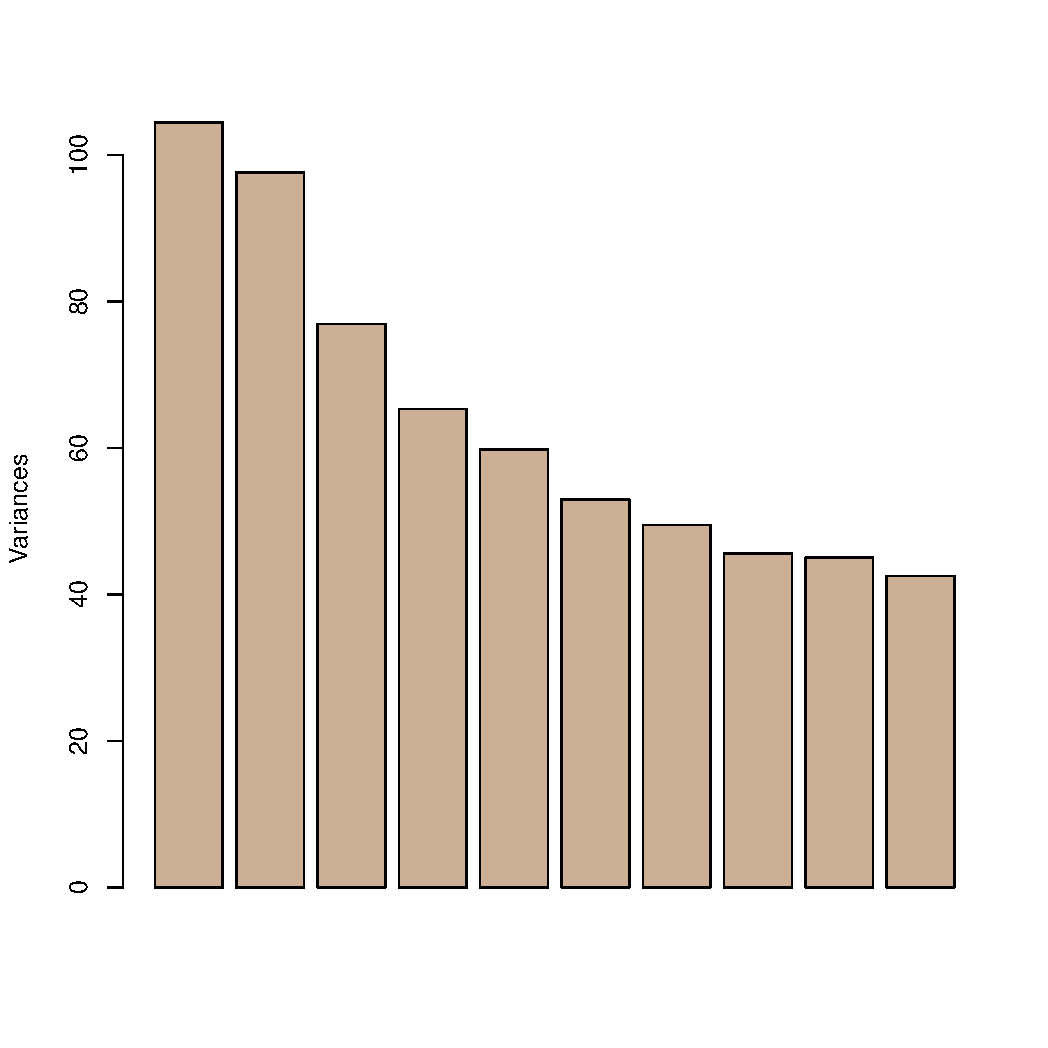
\includegraphics{./figures/PCAvariableplot.pdf}}
\end{center}

\vspace*{-2ex}
        {\scriptsize The variance plot is more gradual than most of our previous examples, but note that all 18 components exceed Kaiser's criterion\\}
\end{frame}



\begin{frame}[fragile]
\frametitle{Clustering on Principal Components}
\framesubtitle{Comparison of Original and New Data Sets}


\begin{center}
{\scriptsize
\begin{tabular}{ccccc}
\multicolumn{5}{c}{\bf Original Sediment Microcosm Data (18 rows, 851 columns)}\\
\multicolumn{5}{c}{ }\\
Treatment & Replicate & OTU 1  & $\ldots$ & OTU 849\\\hline
control   & 1         & 0 or 1   &        & 0 or 1\\
control   & 2         & 0 or 1   &        & 0 or 1\\
(etc.)    & (etc.)    & (etc.)   &        & (etc.) \\      
high      & 5         & 0 or 1   &        & 0 or 1\\
high      & 6         & 0 or 1   &        & 0 or 1\\\hline
\end{tabular}

\vspace{8ex}

\begin{tabular}{ccccc}
\multicolumn{5}{c}{\bf Sediment Microcosm PCA Data (18 rows, 20 columns)}\\
\multicolumn{5}{c}{ }\\
Treatment & Replicate & PC 1      & $\ldots$ & PC 18\\ \hline
control   & 1         & -4.97    &        & $<$ $\pm$0.01\\
control   & 2         & -15.53   &        & $<$ $\pm$0.01\\
(etc.)    & (etc.)    & (etc.)   &        & (etc.) \\      
high      & 5         & 13.81    &        & $<$ $\pm$0.01\\
high      & 6         & 13.10    &        & $<$ $\pm$0.01\\\hline
\end{tabular}


}
\end{center}

\end{frame}


\begin{frame}[fragile]
\frametitle{Clustering on Principal Components}
\framesubtitle{Step 2:  Clustering on the Component Scores}

{\footnotesize
\begin{itemize}

\item This next step requires a good understanding of what is
  accomplished by ordinating the original data using principal
  components.

\vspace{1ex}  
\item A scaled, centered PCA creates a multivariate correlation
  matrix, with the ``best'' correlations contained in the first
  component.  Each successive component contains a smaller fraction
  of ``good'' correlation.

\vspace{1ex}  
\item What we want to do is cluster using a small subset of the
  component scores rather than all the components
  scores. This allows us to focus on just the good multivariate
  correlations.

\vspace{1ex}  
\item In this example, we had 849 variables (OTUs), but {\color{red}
  \tt prcomp} stopped the ordination at 18 components, which contain
  nearly 100\% of the variance.

\vspace{1ex}  
\item The next figure shows the dendrogram for clustering the samples
  using all 18 principal components. I used euclidean distance and
  Ward's minimum variance clustering method. ({\color{red} \tt ward.D} used to duplicate results in Chariton et al.~2014)

\vspace*{1ex}
Note: We don't want to use all components, but it is a
good place to start.

\end{itemize}
}

\end{frame}


\begin{frame}[fragile]
\frametitle{Clustering on Principal Components}
\framesubtitle{Dendrogram Results using 18 Components}

\begin{center}
\resizebox{3in}{!}{
	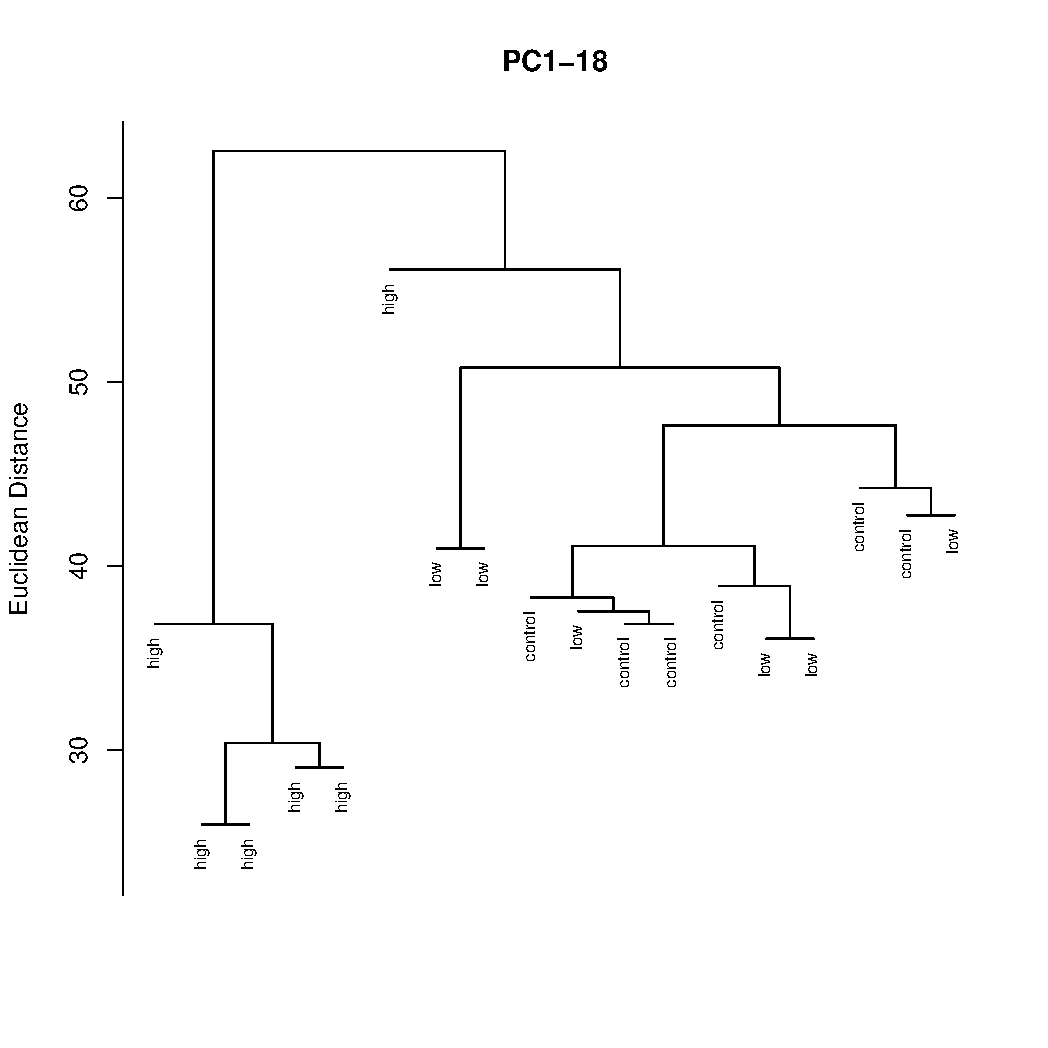
\includegraphics{./figures/hclustPCAall.pdf}}
\end{center}
\end{frame}


\begin{frame}[fragile]
\frametitle{Clustering on Principal Components}
\framesubtitle{Step 3: Identifying Stable Clusters}

{\scriptsize
\begin{itemize}

\item We want to cluster using fewer than 18 component scores.  But
  how many should we select?

\item This is actually a rather difficult question, but the short
  answer is to use the fewest principal components that produce
  ``stable'' clusters (see Ben-Hur and Guyon, 2003).

\item Preliminary evaluation of the 18-component dendrogram shows that
  there are only two {\color{blue} \em treatment} responses (high or
  control$+$low), and one outlier (``high'').

\item Using Association Analysis, we can test whether the separation
  into two groups is statistically significant (FYI: ``eward'' is the
  name of my hierarchical clustering object)

{\scriptsize
\color{red}
\verb%HCgroups = cutree(eward, 2)%\\
\verb%table(HCgroups, treatment)%

\color{blue}
\verb%        treatment%\\
\verb%HCgroups control high low%\\
\verb%       1       6    1   6%\\
\verb%       2       0    5   0%

\color{red}
\verb%chisq.test(HCgroups, treatment) #edited output%\\
\color{blue}
\verb%X-squared = 13.8462, df = 2, p-value = 0.0009848%
}

\end{itemize}
}

\end{frame}


\begin{frame}[fragile]
\frametitle{Dendrogram Results using PC1-PC7}

\begin{center}
\resizebox{4in}{2.8in}{
	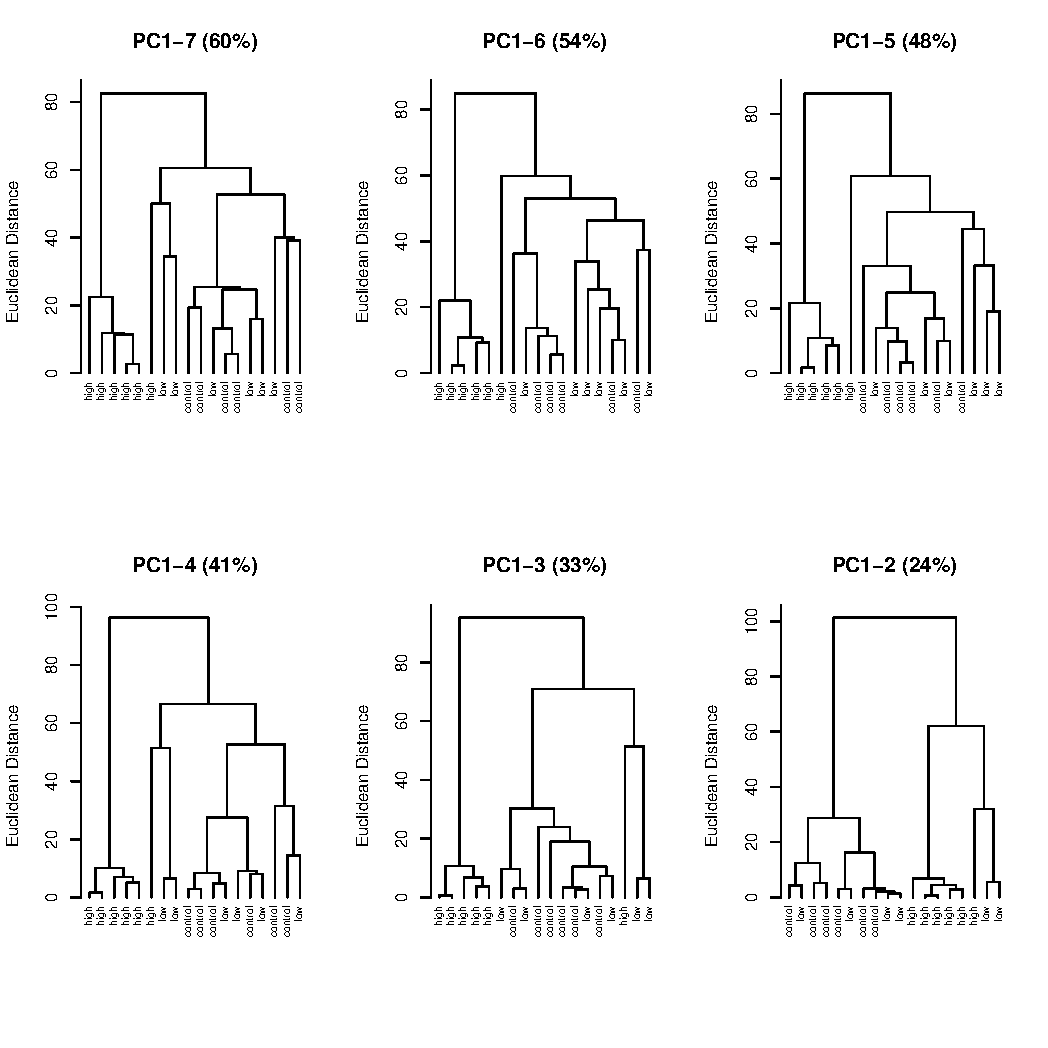
\includegraphics{./figures/hclustPCAsubset.pdf}}
\end{center}

\vspace*{-4ex} {\scriptsize Cycling through all clustering options
  (PC1--PC18, PC1--PC17, PC1--PC16, etc), each have 1
  misclassification until you use only PC1--PC2, which
  has 2 misclassifications. 
{\color{blue} \em You only need PC1--PC3 to produce
  stable clusters\\}
}

\end{frame}


\begin{frame}[fragile]
\frametitle{Clustering on Principal Components}
\framesubtitle{Step 4: Refining Cluster Membership and Checking Significance}

{\footnotesize
\begin{itemize}

\item Once we decide on the number of principal components to use
  (PC1--PC3), it is important to revisit the question of cluster
  membership

\vspace*{1ex}  
\item You can see from the next figure that there are two obvious
  clusters that match treatment groups.  One cluster contains five
  ``high'' treatment samples and the other cluster contains all of the
  control and low samples, plus one high outlier

\vspace*{1ex}  
\item But in the next figure, note that you could also describe the
  data using three clusters.  Two of the clusters show treatment
  effects (high or control/low); the third cluster contains three
  outlier samples.

\vspace*{1ex}  
\item In both cases, the associations between clusters and treatment
  groups are statistically significant (p-value $\le$0.001).

\vspace*{1ex}  
\item Choosing which way to display the results depends on your
  overall goals, but it is usually desirable to discuss outliers
  separately from the treatment effect.

\end{itemize}
}
\end{frame}


\begin{frame}[fragile]
\frametitle{Clustering on Principal Components}
\framesubtitle{Two-Cluster Dendrogram}

\begin{center}
\resizebox{4in}{2.5in}{
	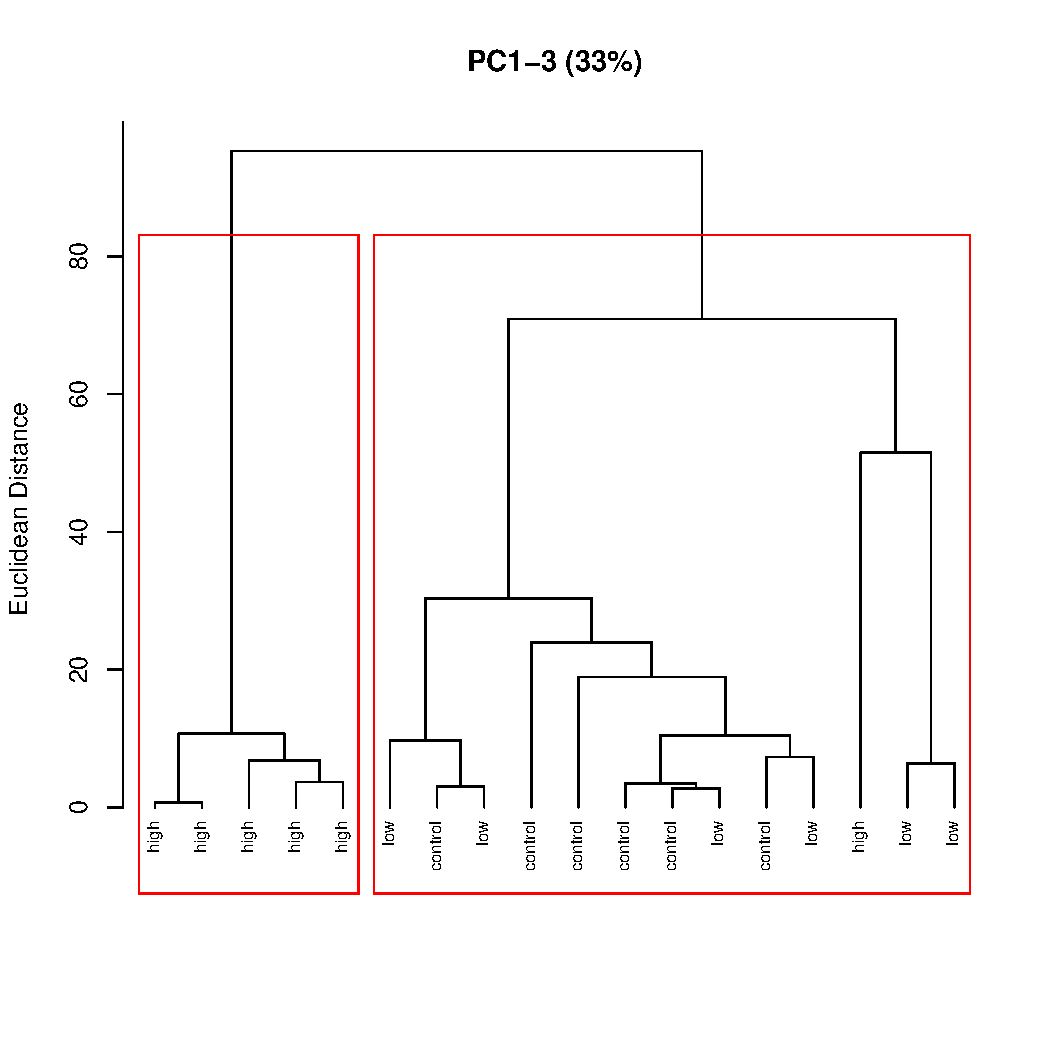
\includegraphics{./figures/hclustPCAbest.pdf}}
\end{center}

\vspace{-6ex}
{\scriptsize \color{red}
\verb%HCgroups = cutree(eward, 2); chisq.test(HCgroups, treatment)%\\

\color{blue}
\verb%X-squared = 13.8462, df = 2, p-value = 0.0009848%\\
}
\end{frame}



\begin{frame}[fragile]
\frametitle{Clustering on Principal Components}
\framesubtitle{Three-Cluster Dendrogram}

\begin{center}
\resizebox{4in}{2.5in}{
	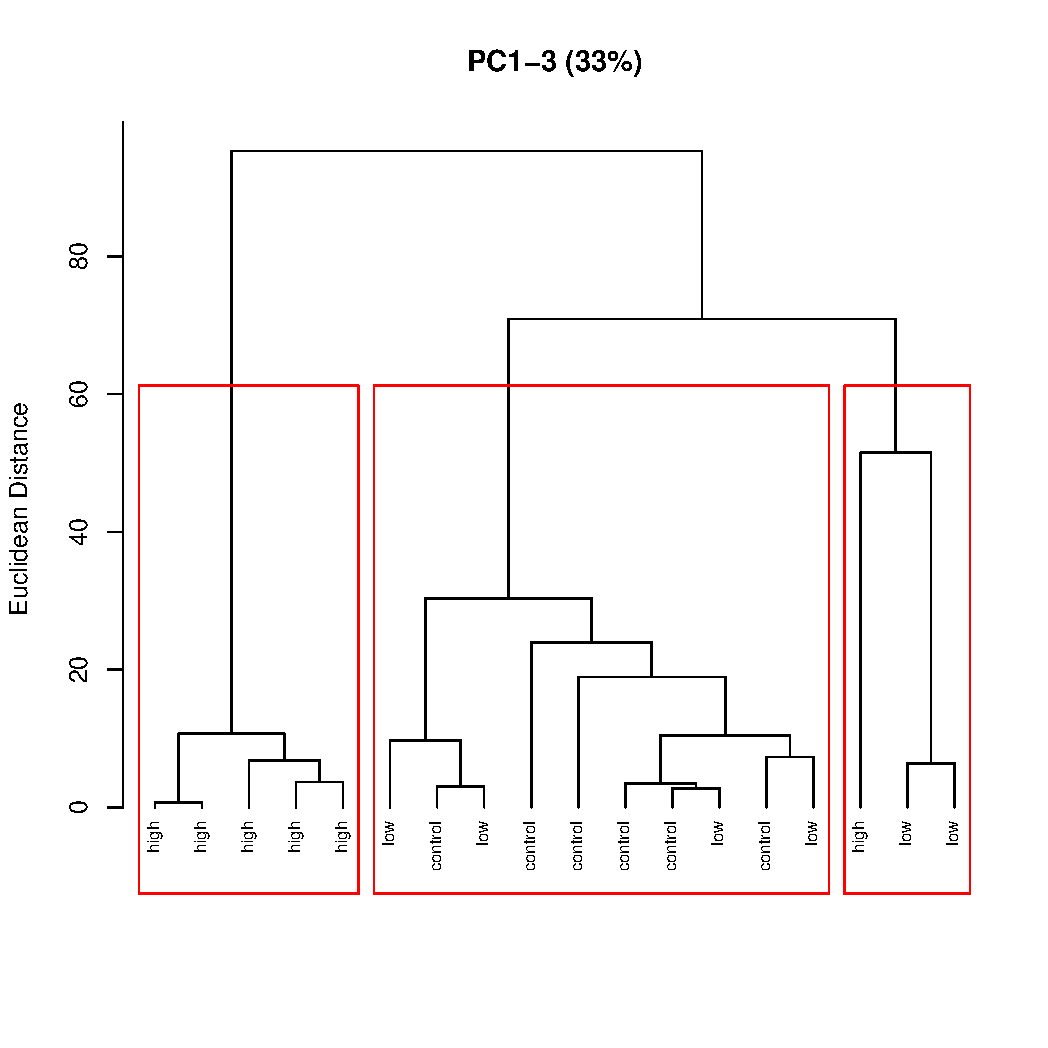
\includegraphics{./figures/hclustPCAbest3.pdf}}
\end{center}

\vspace*{-6ex}
{\scriptsize \color{red}
\verb%HCgroups = cutree(eward, 3); chisq.test(HCgroups, treatment)%\\

\color{blue}
\verb%X-squared = 17.6, df = 4, p-value = 0.001477%\\
}
\end{frame}


\begin{frame}[fragile]
\frametitle{Clustering on Principal Components}
\framesubtitle{Step 5: Interpreting the Results}

{\footnotesize
\begin{itemize}
\item Using this multivariate method, we determined that there were
  only two treatment responses, not the original three.  In addition,
  there was a group of outliers from {\em \color{blue} different}
  treatment groups.

\vspace*{1ex}  
\item To finish the evaluation, we need to know how the original
  variables influenced the first three principal components, and how
  that in turn can be used to describe the cluster groups.

\vspace*{1ex}  
\item An approach that works with some data sets is to show summary
  statistics (e.g., minimum, median, maximum) for each cluster
  group.  But that isn't feasible for presence/absence data.

\vspace*{1ex}  
\item Another approach is to look at the variable scores for the
  components used to cluster the data.  Because there were so many
  OTUs, we need to focus on the ``best'' variables, but defining
  ``best'' is somewhat arbitrary.

\end{itemize}
}
\end{frame}

\begin{frame}[fragile]
\frametitle{Clustering on Principal Components}

%%% from edited PCA_variables.ods

{\scriptsize
\begin{center}
\begin{tabular}{lc|lc|lc}
\multicolumn{6}{c}{\bf Best Negative Variable Scores in PC1-PC3}\\
OTU	& PC1	  & OTU 	& PC2	        & OTU 	        & PC3\\ \hline
M.5324	& -0.085  & M.521	        & -0.087	& M.33548	& -0.082\\
M.17875	& -0.083  & F.671	        & -0.087	& M.29634	& -0.076\\
M.18385	& -0.083  & uk.euk.3152	& -0.087	& uk.euk.9604	& -0.074\\
M.34715	& -0.083  & S.3978	& -0.087	& M.10729	& -0.074\\
M.25065	& -0.082  & S.7008	& -0.087	& M.4300	& -0.073\\
M.28527	& -0.082  & M.7687	& -0.087	& R.848	        & -0.071\\
uk.euk.6428 & -0.082 & S.9894	& -0.087	& uk.euk.422	& -0.071\\
M.1091	& -0.081  & S.10341	& -0.087	& S.947	        & -0.071\\
M.15718	& -0.080  & S.13318	& -0.087	& uk.euk.1428	& -0.071\\
M.25537	& -0.079  & S.15201	& -0.087	& uk.euk.378	& -0.071\\ \hline
\multicolumn{6}{l}{ }\\					
\multicolumn{6}{l}{ }\\					
\multicolumn{6}{c}{\bf Best Positive Variable Scores in PC1-PC3}\\
OTU	& PC1	  & OTU 	& PC2	        & OTU 	        & PC3\\ \hline
R.30870	& 0.077	  & M.5776	& 0.052		& uk.euk.5340	& 0.088\\
A.11234	& 0.073	  & M.4361	& 0.048		& uk.euk.4435	& 0.084\\
A.5381	& 0.068	  & S.37132	& 0.044		& uk.euk.8723	& 0.081\\
R.9197	& 0.066	  & M.15282	& 0.041		& M.35761	& 0.080\\
S.3563	& 0.065	  & uk.euk.35868 & 0.040	& M.35148	& 0.076\\
M.37060	& 0.060	  & M.10534	& 0.040		& M.20011	& 0.075\\
M.37021	& 0.057	  & M.25299	& 0.039		& R.7994	& 0.075\\
R.1633	& 0.056	  & M.588	& 0.038		& A.25541	& 0.075\\
R.28351	& 0.056	  & F.35789	& 0.037		& M.29451	& 0.075\\
S.20330	& 0.056	  & uk.euk.28316 & 0.037	& M.26907	& 0.075\\ \hline
\end{tabular}
\end{center}
}
\end{frame}


\iwsframe{Clustering on Principal Components}{OTUs Translated into Biotic Richness, from Chariton, et al.}
\begin{center}
\resizebox{2.5in}{!}{
	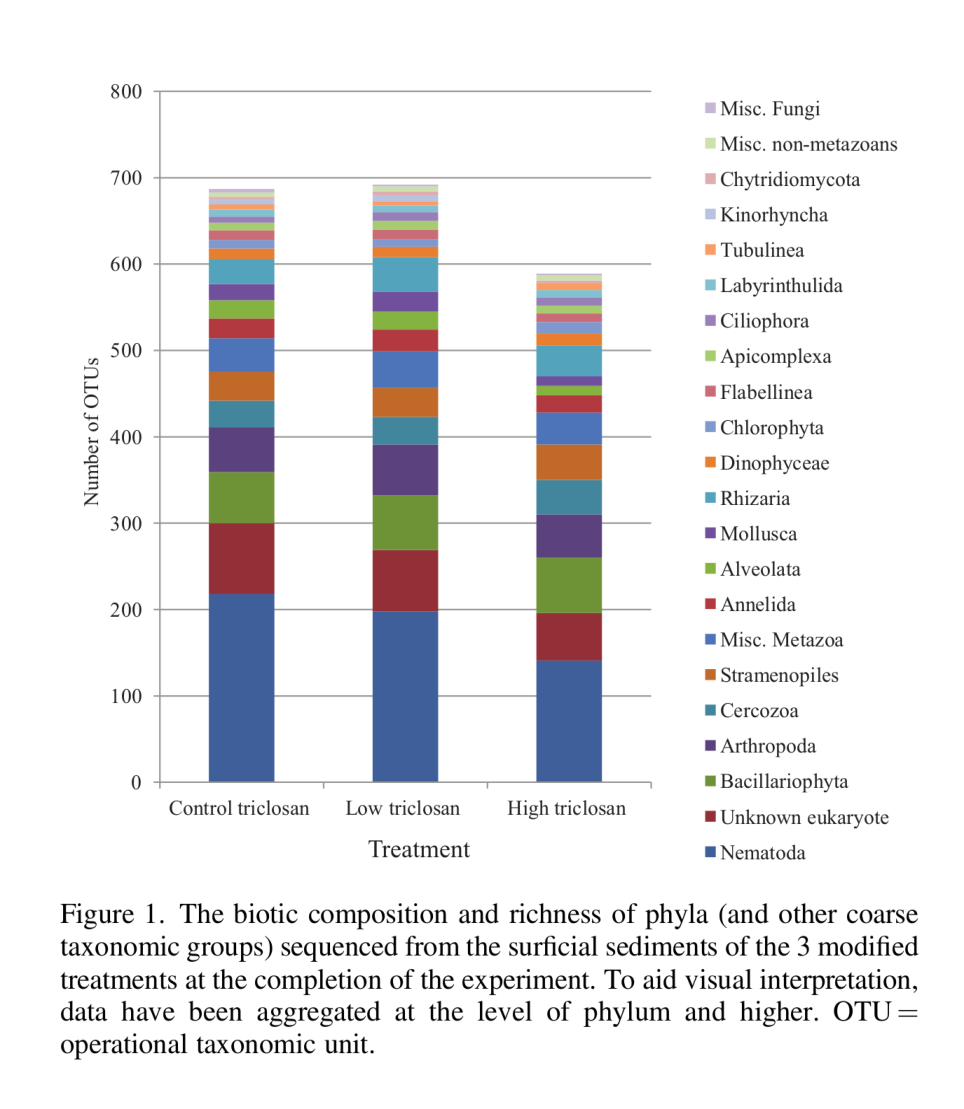
\includegraphics{./figures/chair_fig1.pdf}}
\end{center}
\end{frame}


\iwsframe{Clustering on Principal Components}{Plotting the Samples by PC Scores}

\hspace*{-0.5in}
\resizebox{5in}{!}{
	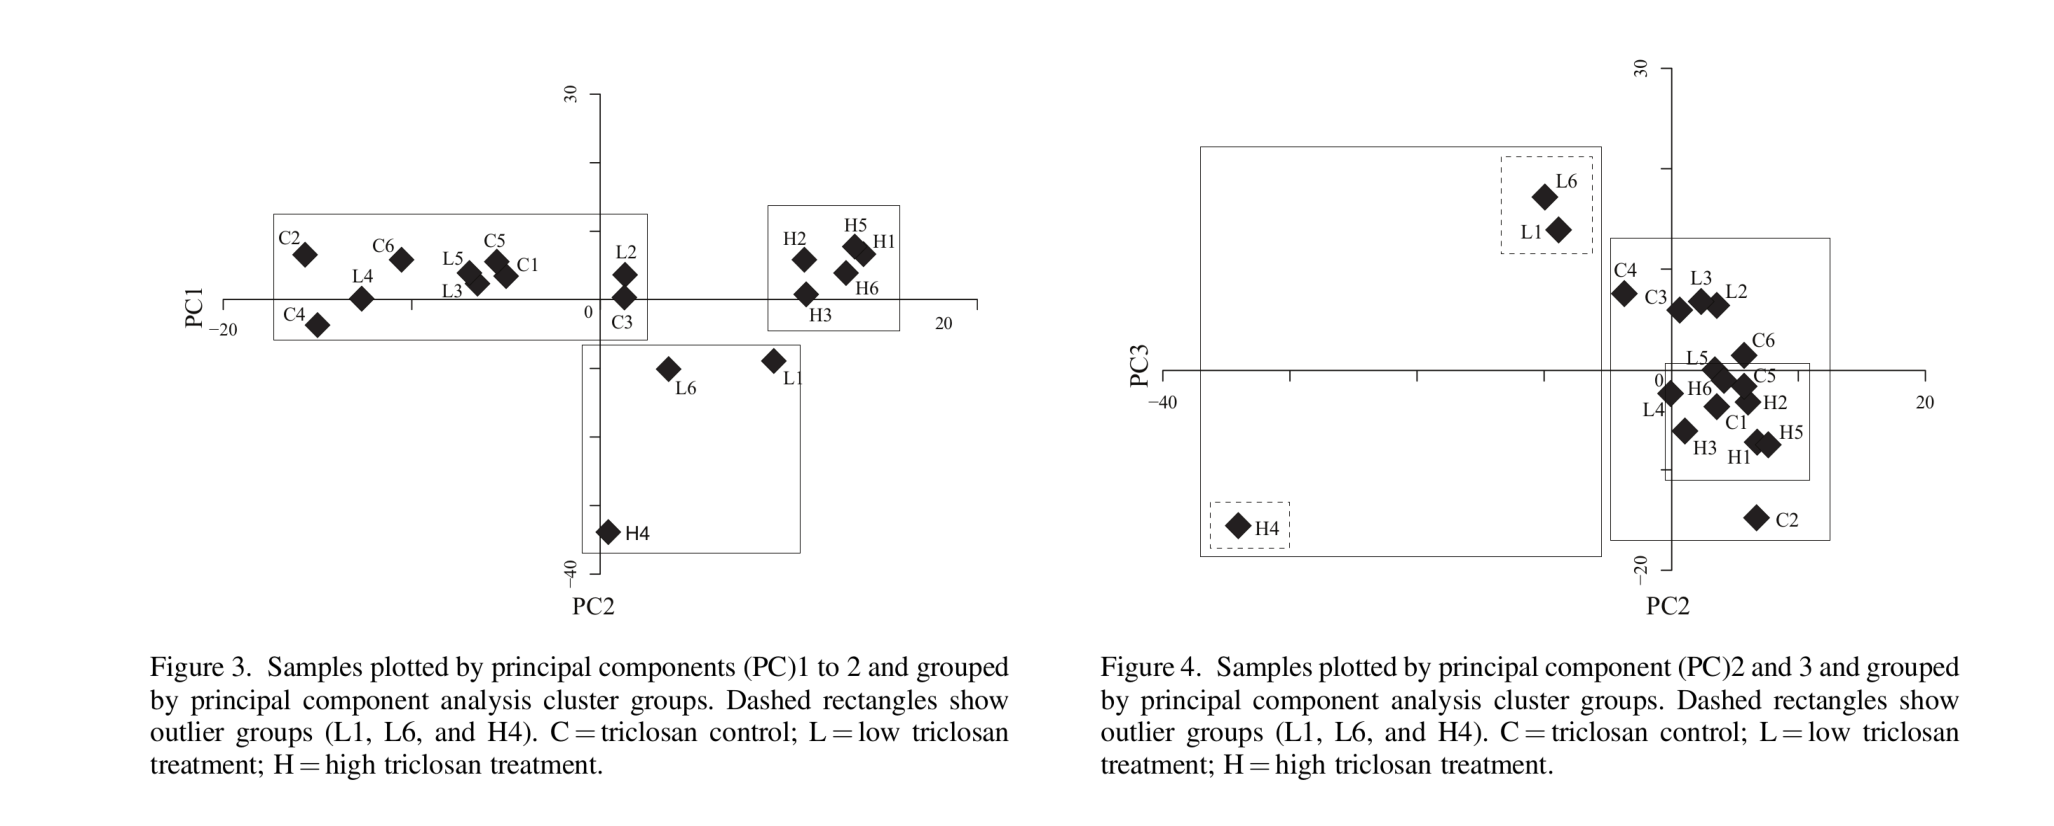
\includegraphics{./figures/chair_fig3.pdf}}

\end{frame}
\end{document}
\end

